\documentclass[11pt,a4paper]{article}
\usepackage[T1]{fontenc}
\usepackage{amsmath,amssymb,amsthm}
\usepackage[margin=1in]{geometry}
\usepackage{longtable,booktabs,array,calc}
\usepackage{graphicx}
\usepackage{float}
\floatplacement{figure}{H}
\usepackage{needspace}
\allowdisplaybreaks[1]
\clubpenalty=10000
\widowpenalty=10000
\raggedbottom
\usepackage{fvextra}
\DefineVerbatimEnvironment{verbatim}{Verbatim}{breaklines=true,fontsize=\small}
\usepackage{xurl}
\usepackage[hidelinks]{hyperref}
\hypersetup{pdftitle={Fate Contagion and Termination Criteria for the
Juggler Map},pdfauthor={Philippe
Cochin},pdfsubject={Mathematics preprint}}
\urlstyle{tt}
\setlength{\emergencystretch}{3em}
\setlength{\LTpre}{1em}
\setlength{\LTpost}{1em}
\setlength{\tabcolsep}{4pt}
\renewcommand{\arraystretch}{1.12}
\providecommand{\tightlist}{\setlength{\itemsep}{0pt}\setlength{\parskip}{0pt}}
\providecommand{\passthrough}[1]{#1}
\setcounter{secnumdepth}{-1}
\title{Fate Contagion and Termination Criteria for the Juggler Map}
\author{Philippe Cochin \\ \texttt{philippe@cochin.fr}}
\date{9 September 2026}
\begin{document}
\maketitle
\begin{abstract}

The Juggler map sends an even positive integer to the integer part of
its square root and an odd positive integer to the integer part of its
three-halves power. We prove that every nonempty set \(A\) closed under
taking preimages satisfies
\(\sum_{n\in A,\,n\le x}1/n\ge c(\log x)^\lambda\), for all sufficiently
large \(x\) and every \(0<\lambda<\lambda^{**}\), where
\(\lambda^{**}\approx0.4926\) is an explicitly specified root. Thus
every realized cycle basin and the set of unbounded orbits, if nonempty,
obey this lower bound. The proof combines exact inverse intervals, a
monotone parity sweep, classical exponential-sum estimates, and a finite
list of disjoint parity productions.

For any fixed \(N_0\ge2\) such that every start in \([1,N_0]\) reaches
\(1\), universal termination is equivalent to an eventual-entry
statement: all but \(O(y(\log y)^{-e})\) odd starts in \((y,2y]\) enter
\([1,N_0]\), for some \(e>1-\lambda^{**}\). We give sufficient
parity-cylinder and exponential-moment hypotheses at depth
\(O(\log\log y)\) for a stronger statement with a time bound. These
hypotheses remain unproved. A first-letter decomposition identifies the
contribution of failures beginning with two odd steps, and an abstract
production model describes possible improvements of the exponent. A
separate appendix gives a conditional exponent \(0.5392\). Selected
combinatorial lemmas are formalized in Lean 4; the analytic estimates
are mathematical arguments outside the formalization, and the numerical
experiments are observations. Neither universal termination nor the
exclusion of a nontrivial cycle or an unbounded orbit is established.

\end{abstract}

\textbf{2020 Mathematics Subject Classification:} 11B37, 11L07, 37P99.

\textbf{Keywords:} Juggler map; preimage sets; logarithmic counting;
parity cylinders; integer dynamics.

\section{1. Introduction}\label{introduction}

For a positive integer \(n\), define \[
J(n)=\begin{cases}
\lfloor\sqrt n\rfloor,&n\text{ even},\\
\lfloor n^{3/2}\rfloor,&n\text{ odd}.
\end{cases}
\]

The Juggler sequence was introduced by Pickover {[}1{]} and is sequence
A094683 of the OEIS {[}2{]}. Starting from any positive integer, the
orbit under \(J\) appears always to reach \(1\); this has been verified
for all starts up to \(3.5\cdot 10^8\) {[}11{]}. The map belongs to the
family of floor-power maps, and its dynamics resembles the \(3x+1\)
problem {[}3, 4{]} in one respect and differs from it in another. The
resemblance: a parity decides whether the orbit goes up or down, and the
heuristic model of the orbit is a random walk with negative drift, here
on the scale \(\log\log n\) with steps \(+\log_2 3-1\) (odd) and \(-1\)
(even). The difference: the Juggler map moves by \emph{powers}, so a
single contracting certificate sends \(n\) to \(n^{e}\) with \(e<1\),
and the one-step preimages of an integer are not a residue class but an
interval.

This paper is about the second feature and what it forces. The narrative
has four steps.

\emph{Contagion.} Let \(R\) be the set of starts that reach \(1\), \(F\)
its complement, \(B(C)\) the basin of a nontrivial cycle \(C\), and
\(D\) the set of divergent starts. Each is \emph{backward-closed}: if
\(J(n)\) belongs to it, so does \(n\). Theorem 1 proves that every
nonempty backward-closed set is large in logarithmic density, with an
explicit exponent, by a downward recursion over two exact productions
and the finite composites in Appendix D. Applied to the fate classes: if
a single start fails to reach \(1\), the failures have logarithmic count
\(\gg(\log x)^\lambda\) and, on infinitely many dyadic blocks, natural
density \(\gg(\log y)^{\lambda-1}\), for every
\(0<\lambda<\lambda^{**}\). This excludes no fate; it fixes the
quantitative shape of the trichotomy.

\emph{Odd generation.} A set that is closed both forwards and backwards
and avoids \(1\) is the \(E\)-forest (iterated even preimages) over its
odd members, and its odd members are the odd preimages of its
intersection with the sparse set \(S=\{\lfloor m^{3/2}\rfloor:\ m\
\text{odd}\}\) (Theorem 2). An arbitrary failure set is thereby replaced
by sparse odd-image seeds together with deterministic even ancestry.
This is the geometry that the later sections use.

\emph{The almost-all equivalence.} Tao {[}6{]} proved that almost all
Collatz orbits (in logarithmic density) attain almost bounded values,
with a target \(f(N)\to\infty\) arbitrarily slowly. For the Juggler map,
contagion and odd generation together turn a bounded-target statement
into the conjecture: every positive integer reaches \(1\) if and only if
all but \(O(y(\log y)^{-e})\) odd starts in \((y,2y]\) enter
\([1,N_0]\), for some \(e>1-\lambda^{**}\approx0.5074\) (Theorem 3). The
threshold is the complement of the contagion exponent. The Collatz
preimage lower bound of Krasikov--Lagarias {[}7{]}, discussed with its
target restriction in Section 1.3, does not by itself yield this
implication.

\emph{Sufficient estimates at growing depth.} The exponent walk needs to
fall by \(L(y)=\log_2(\log(2y)/\log N_0)\) to put a start in \((y,2y]\)
below the floor. A Chernoff estimate counts words whose walk fails to
cross this level by depth \(\lceil CL(y)\rceil\). Turning this word
count into a count of integer starts requires additional arithmetic
information. Sections 8--9 give three sufficient forms of that
information: upper bounds on bad cylinders, one-sided control of their
continuations, and a bound on one exponential moment of live starts. A
bound on tilted odd shares implies the moment bound. None is established
here.

The first-letter decomposition in Section 6 relates the remaining
\(OO\)-contribution to failures at a larger scale. Section 10 connects
this term with live-start counts and states a uniformity requirement for
a particular cylinder-counting method. These are reductions and
limitations of the stated estimates, not necessity results for every
possible proof of termination.

\subsection{1.1 Main results}\label{main-results}

Write \(\ell_A(u,v]=\sum_{n\in A,\,u<n\le v}1/n\). Throughout,
\(N_0\ge2\) is any integer with \([1,N_0]\subseteq R\) (the
Lean-verified value is \(260\); the certified computational value is
\(3.5\cdot 10^8\) {[}11{]}).

\textbf{Theorem 1 (fate contagion).} Let \(A\subseteq\mathbb N\) be
nonempty and backward-closed, and let
\(0<\lambda<\lambda^{**}\approx0.4926\), the root of \[
2^{-\lambda}+\tfrac19(\tfrac38)^\lambda+\tfrac29(\tfrac34)^\lambda
 +\sum_{k=2}^{6}3^{-(k+1)}\left(\tfrac12(\tfrac34)^k\right)^\lambda=1.
\tag{1.1}
\] (The \(V_5\) truncation of the first seven terms is \(0.4924\); the
\(V_4\) truncation of the first six terms is \(0.4916\); the \(V_3\)
truncation of the first five is \(0.4891\); the \(OEOEE\) truncation of
the first four is \(0.4801\); the pairing-only root of the first three
is \(0.4480\).) There are \(c>0\) and \(x_0\), depending on \(A\) and
\(\lambda\), with \[
\sum_{\substack{n\in A\\ n\le x}}\frac1n\ \ge\ c\,(\log x)^{\lambda}
\qquad(x\ge x_0).
\] Consequently each fate class realized by at least one start ---
\(R\), the basin of any existing nontrivial cycle, the divergent set ---
satisfies this bound, and on infinitely many dyadic blocks has natural
density \(\gg(\log y)^{\lambda-1}\). (Theorem 5.3, Corollaries 5.4,
5.5.)

The finite productions in Section 5.7 and Appendix D give this exponent.
Their formal infinite series has limiting root \(0.4927\), but only the
stated finite truncation is used here. The ideal characteristic model in
Proposition 5.12 has root \(1\); the other run-model values, including
\(0.8414\), are conditional calculations and are not attained density
exponents.

\textbf{Theorem 2 (odd generation).} Let \(A\) be forward- and
backward-closed with \(1\notin A\). Every \(n\in A\) reaches by a
possibly empty sequence of even steps to an odd member \(m\ge 3\) of
\(A\); for odd \(n\), \(n\in A\iff\lfloor n^{3/2}\rfloor\in A\); and
\(A\ne\emptyset\) iff \(A\) contains the image
\(\lfloor m^{3/2}\rfloor\) of some odd \(m\ge 3\). In particular every
positive integer reaches \(1\) iff no odd image fails to. (Theorem 6.1;
Lean.)

\textbf{Theorem 3 (the conjecture as an almost-all statement).} The
following are equivalent: (i) every positive integer reaches \(1\); (ii)
for some \(0<\lambda<\lambda^{**}\), the starts \(n\le x\) whose orbit
never enters \([1,N_0]\) have logarithmic count
\(o((\log x)^{\lambda})\); (iii) for some
\(e>1-\lambda^{**}\approx0.5074\) and all large \(y\),
\(\#\{n\ \text{odd}\in(y,2y]:\ n\notin R\}\le y(\log y)^{-e}\).
(Corollary 7.1, Theorems 7.2, 7.3.)

\textbf{Theorem 4 (the frontier reduction).} Let
\(L(y)=\log_2(\log 2y/\log N_0)\), \(d(y)=\lceil CL(y)\rceil\),
\(p_C=(1-1/C)/\log_2 3\), \(e(C)=C\,D(p_C\|\tfrac12)/\ln 2\), and
\(e_q^{\rm Az}(C)=2(C(1-q\log_2 3)-1)^2/
(C(\log_2 3)^2\ln2)\). Assume \(C\ge5\). The following hypotheses give
the indicated, case-dependent bounds. Each implies (iii) of Theorem 3
whenever its displayed rate exceeds \(1-\lambda^{**}\):

\begin{enumerate}
\def\labelenumi{(\alph{enumi})}
\item
  \emph{cylinder form} \(\mathrm H(C,A)\): no \(O\)-rooted, \(L(y)\)-bad
  itinerary cylinder of depth \(d(y)\) exceeds its fair share
  \(2^{-(d-1)}y/2\) among odd starts by more than \(y(\log y)^{-A}\),
  \(A>C+e(C)\) (Theorem 8.3), giving \(e(C)-\varepsilon\) and hence the
  conjecture for \(C\ge19\) using Theorem 1 (or \(C\ge18\) under
  Appendix C);
\item
  \emph{one-sided form} \(\mathrm H_q(C,A)\), with \(0<q<\log 2/\log 3\)
  and \(C>1/(1-q\log_2 3)\): every \(L(y)\)-bad cylinder of depth
  \(1\le t<d(y)\) sends at most a fraction \(q\) of its members, plus
  \(y(\log y)^{-A}\), to an odd next state (Theorem 9.1;
  \(A>C+e_q^{\rm Az}(C)\)), giving \(e_q^{\rm Az}(C)-\varepsilon\); at
  \(q=0.55\), \(C\ge41\) crosses Theorem 1's threshold;
\item
  \emph{pressure form} \(\mathrm P_\theta(C)\):
  \(\frac1N\sum_{n\ \mathrm{odd}\in(y,2y],\ \tau(n)>d}e^{\theta o_d(n)}\le(\tfrac12(1+e^{\theta}))^{d}e^{o(d)}\)
  at \(\theta=\log(p_C/(1-p_C))\), with \(N=y/2\), where \(\tau\) is the
  entrance time into \([1,N_0]\) and \(o_d\) the odd count of the first
  \(d\) letters; this gives \(e(C)-\varepsilon\). Its biased
  \emph{no-momentum form}, for \(0<q<p_C<1\),
  \(\sum_{t<d}(s_\theta(t)-q)^+=o(d)\) gives
  \(C D(p_C\|q)/\ln2-\varepsilon\) only at the optimizing tilt
  \(\theta=\log(p_C(1-q)/(q(1-p_C)))\) (Theorem 9.2, Proposition 9.3).
\end{enumerate}

None of these hypotheses is proved here. A bounded loss at each of
\(o(\log\log y)\) exceptional depths can be absorbed in the moment
criterion. The tower comparison and finite-depth model in Section 9.3
describe the scope of this argument; neither is an arithmetic necessity
theorem.

\textbf{Theorem 5 (first-letter decomposition).} A two-way closed set
has the disjoint first-letter decomposition of Section 6.2. In the
normalization used there, its logarithmic density satisfies (6.1), with
the stated boundary error. For the failure set \(F\), the free term
\(\psi_F\) is a known normalization factor times the decreasing limit of
the live proportion among \(OO\)-type starts (Proposition 10.1). Each
sufficient estimate of Theorem 4 bounds this term at its stated
logarithmic rate. The upper recursion obtained by bounding the fiber
weights gives decay estimates with a critical exponent; that upper
inequality alone does not force the failure set to be empty (Corollary
10.2).

\textbf{Proposition (depth-uniformity budget).} Suppose the error bound
available for each cylinder is \(K2^{\kappa d}y^{1-\delta_0 2^{-cd}}\),
with \(K,\delta_0,c>0\) and \(\kappa\ge0\) independent of the depth. The
resulting union-bound error is negligible at depth
\(C\log_2\log y+O(1)\) precisely when \(cC<1\) (Proposition 10.3). This
is a criterion for the available error majorant, not a lower bound on
the actual discrepancy.

Under a localization of the triple parity discrepancy of nested floor
powers to sub-dyadic intervals --- stated as an explicit hypothesis in
Appendix C; it is Theorem 4.12 of the working draft {[}12{]}, and its
status is described there --- the exponent of Theorem 1 improves to
\(\lambda^{***}\approx0.5392\), the rate threshold of Theorem 3 to
\(0.4608\), and the least depth constant of Theorem 4 to \(C\ge 18\).
Nothing in Sections 2--12 depends on Appendix C.

\subsection{1.2 The three fates as currently
constrained}\label{the-three-fates-as-currently-constrained}

The three fate classes are the three Moirai: Atropos cuts the thread
(the class \(R\)), Lachesis measures an allotted length (a cycle basin),
Clotho spins without end (divergence). What is known about each, all
from outside this paper:

\begin{itemize}
\tightlist
\item
  \emph{Atropos.} Every \(n\le N_0=3.5\cdot 10^8\) reaches \(1\)
  (independently certified computation, {[}11, Section 5{]}); the
  Lean-verified floor is \(N_0=260\). Paper B {[}12{]} proves that
  \(7/8\) of all starts descend below themselves within five steps, with
  a power saving on dyadic blocks.
\item
  \emph{Lachesis.} A nontrivial cycle has minimum above
  \(3.5\cdot 10^8\) and period at least \(780239\) {[}11{]}; it has at
  least four even steps; if \(3^o/2^L=1+\Lambda\), its odd share is
  \(\log 2/\log 3+\log(1+\Lambda)/(L\log3)\), strictly above but, under
  the finance bound, very near the critical zero-drift share.
\item
  \emph{Clotho.} A divergent orbit has unbounded exponent walk; its
  record jumps are quantized to the \(\log_2 3\) lattice {[}11{]}.
  Nothing excludes it.
\end{itemize}

Theorem 1 adds one sentence to each: whichever of the three acts at all
acts on a set of logarithmic count \(\gg(\log x)^\lambda\) for every
\(0<\lambda<\lambda^{**}\).

\subsection{1.3 Related work}\label{related-work}

\emph{Collatz parity vectors.} Terras {[}4{]} and Everett {[}5{]} showed
that the first \(k\) parities of the Collatz orbit of \(n\) are
determined by \(n\bmod 2^k\) and equidistributed exactly, and deduced
that almost all starts have finite stopping time (descend below
themselves). The analogous exact statement fails for the Juggler map:
the parities of \(\lfloor n^{3/2}\rfloor\),
\(\lfloor\lfloor n^{3/2}\rfloor^{3/2}\rfloor\), \(\dots\) are
Diophantine, not algebraic, and their equidistribution is proved only to
depth four (Paper B, {[}12{]}).

\emph{Tao's theorem.} Tao {[}6{]} proved that for any \(f(N)\to\infty\),
almost all Collatz orbits (in logarithmic density) attain a value below
\(f(N)\). The bounded-target version is not available, and the renewal
machinery through the Syracuse random variables is the heart of the
proof. Section 7.1 explains, as a structural analogy and not as a
transfer of methods, which parts of that picture change for the Juggler
map.

\emph{Preimage trees.} Krasikov and Lagarias {[}7{]} obtain an
\(x^{0.84}\) lower bound for Collatz preimage counts, for targets not
divisible by \(3\) and sufficiently large \(x\). Such a lower bound
alone does not give a divergent logarithmic count: a set whose counting
function is \(O(x^{0.84})\) has a convergent reciprocal sum. It
therefore cannot by itself contradict a failure estimate of size
\(y(\log y)^{-e}\). For Juggler, Theorem 1 gives a divergent logarithmic
lower bound for every nonempty preimage set.

\emph{Floor-power maps and exponential sums.} The parity of
\(\lfloor n^{3/2}\rfloor\) along an arithmetic progression is a question
about \(\{n^{3/2}/2\}\); Section 4 uses only an elementary sweep
argument and, on even blocks, the second-derivative test with Vaaler's
approximation {[}10{]}, as for Piatetski-Shapiro sequences. Deeper
nesting is Paper B's subject.

\emph{Companion papers.} Paper A {[}11{]} proves period lower bounds for
a hypothetical cycle from a certified descent floor (cycle financing,
walk-charge envelope); Paper B {[}12{]} proves parity equidistribution
of nested floor powers to depth four with power savings. Neither is
reproved here; both enter as citations, and one statement of the type
Paper B proves enters Appendix C as an explicit hypothesis.

\subsection{1.4 Verification}\label{verification}

Statements carry one of four roles. \emph{Lean}: the exact combinatorial
layer is formalized in Lean 4; the root
\texttt{\nolinkurl{formal/Problems/JugglerFatePaper.lean}} imports
exactly the twelve modules this paper cites and builds with
\texttt{lake\ build\ Problems.JugglerFatePaper}, without
\texttt{\nolinkurl{sorry}} and without
\texttt{\nolinkurl{native_decide}};
\texttt{\nolinkurl{formal/AxiomCheckPaperC.lean}} prints the axiom
dependencies of every cited name and
\texttt{\nolinkurl{AxiomCheckPaperC.expected}} records them ---
Mathlib's \texttt{\nolinkurl{propext}},
\texttt{\nolinkurl{Classical.choice}}, \texttt{\nolinkurl{Quot.sound}}
and nothing else (names in Appendix A). \emph{Human proof}: the analytic
and probabilistic counting. \emph{Verified computation}: exact integer
computations (the descent floor is Paper A's; the closure of \([1,260]\)
under the two productions up to \(10^9\) is computed here).
\emph{Observation}: numerical experiments that check hypotheses and
constants; they prove nothing and are labelled wherever they appear.

\begingroup\small

\begin{longtable}[]{@{}
  >{\raggedright\arraybackslash}p{(\linewidth - 2\tabcolsep) * \real{0.5000}}
  >{\raggedright\arraybackslash}p{(\linewidth - 2\tabcolsep) * \real{0.5000}}@{}}
\toprule\noalign{}
\begin{minipage}[b]{\linewidth}\raggedright
Result
\end{minipage} & \begin{minipage}[b]{\linewidth}\raggedright
Status
\end{minipage} \\
\midrule\noalign{}
\endhead
\bottomrule\noalign{}
\endfoot
\bottomrule\noalign{}
\endlastfoot
Fate classes closed; trichotomy; exclusion (Lemma 2.1) & Lean \\
Even block is an interval (Lemma 3.1) & Lean \\
\(OE\) fiber is an interval; cell identity (Lemma 3.2) & Lean \\
Odd generation (Theorem 6.1) & Lean \\
Envelope descent into the floor (Lemma 8.1) & Lean, on Paper A's power
envelope \\
Sweep lemma (Lemma 4.1), both half-cell conventions & Lean \\
Monotone pairing (Lemma 4.1') & Lean \\
Fiber parity, thin fibers (Lemmas 4.2--4.3) & human proof \\
Block average (Proposition 4.4), asymptotic & human proof \\
Share law and its three corollaries (Lemma 4.5, Corollary 4.6) & human
proof \\
Cube fibers full or alternating (Lemma 4.7) & Lean \\
Recursion lemma (Lemma 5.1) & Lean \\
Seed (Lemma 5.2) & Lean \\
Contagion (Theorem 5.3) & human proof \\
Least failure is \(OO\)-type; first-letter trichotomy (Proposition
6.3(i), Section 6.2) & Lean \\
First-letter identity (6.1) & human proof (exact combinatorics) \\
Tao-type rate implies the conjecture (Theorem 7.2), with the contagion
bound of Theorem 5.3 as a hypothesis & Lean \\
Almost-all equivalence (Theorem 7.3) & human proof \\
Chernoff count of bad words (Lemma 8.2, exact form) & Lean \\
Theorem 8.3, explicit form \(y\Lambda^{-e(C)}+2\Lambda^Cy(\log y)^{-A}\)
at every \(y\) & Lean; the \(\varepsilon\)-absorption into the displayed
form is human \\
Pressure form (Theorem 9.2, exact: a pressure bound \(Na_\theta^dE\)
gives at most \(Ne^{-dD(p_C\Vert 1/2)}E\) live starts) & Lean, on the
live weight \\
Pressure telescoping (Proposition 9.3) & Lean, on the word-weight
framework \\
Azuma and exponential-moment arguments (Sections 8--10, except Lemma
8.2, Theorem 8.3, Theorem 9.2 and Proposition 9.3 in their exact forms)
& human proof \\
Localized triple discrepancy (Appendix C) & hypothesis, conditional \\
Numerical experiments (Section 11) & observation \\*
\end{longtable}

\endgroup

\begin{figure}
\centering

\includegraphics[width=0.88\linewidth,height=\textheight,keepaspectratio]{figures/paper_c_dependencies.png}
\caption{Logical dependencies. The arithmetic lemmas feed the contagion
theorem. Each unproved parity hypothesis is a sufficient route to a
time-bounded live count, which implies eventual termination only at the
stated rate. No converse time bound is asserted.}
\end{figure}

\section{2. Fate classes and closure}\label{fate-classes-and-closure}

\(\mathbb N=\{1,2,\dots\}\). For \(A\subseteq\mathbb N\) and
\(0\le u<v\) write \[
\ell_A(u,v]=\sum_{\substack{n\in A\\ u<n\le v}}\frac1n,\qquad
g_A(t)=\ell_A\bigl(e^{t/2},e^{t}\bigr].
\] For \(A=\mathbb N\), \(g(t)=t/2+O(e^{-t/2})\).

\textbf{Definition.} \(A\) is \emph{backward-closed} if \(J(n)\in A\)
implies \(n\in A\), and \emph{forward-closed} if \(n\in A\) implies
\(J(n)\in A\).

\textbf{Lemma 2.1 (fate classes).} Let \(R=\{n:\exists k,\ J^k(n)=1\}\),
\(F=\mathbb N\setminus R\), \(B(m)=\{n:\exists k,\ J^k(n)=m\}\), and
\(D=\{n:\forall B\ \exists k,\ J^k(n)>B\}\). Each of \(R,F,B(m),D\) is
backward-closed; \(R,F,D\) are also forward-closed. Every \(n\ge 1\)
lies in \(R\), or in \(B(m)\) for some \(m\ge 2\) on a cycle, or in
\(D\), and these possibilities exclude one another.

\emph{Proof.} Backward closure is the definition of each set (for \(D\):
\(J^k(J(n))=J^{k+1}(n)\)). Forward closure of \(R\): if \(J^k(n)=1\)
then \(J^{k-1}(J(n))=1\) for \(k\ge 1\), and \(J(1)=1\). Forward closure
of \(D\): given \(B\), pick \(k\) with \(J^k(n)>\max(B,n)\); then
\(k\ge 1\) and \(J^{k-1}(J(n))>B\). Trichotomy: a bounded orbit repeats,
a repeat is a cycle, a cycle through \(1\) is the fate \(R\). Exclusion:
an orbit that reaches \(1\) or enters a cycle is bounded; an orbit that
reaches \(1\) and passes through a cycle state \(m\ge 2\) of period
\(L\) would force \(m=J^{qL}(m)=1\). Lean:
\texttt{\nolinkurl{reachesOne_backwardClosed}},
\texttt{\nolinkurl{not_reachesOne_backwardClosed}},
\texttt{\nolinkurl{ancestor_backwardClosed}},
\texttt{\nolinkurl{escapes_backwardClosed}},
\texttt{\nolinkurl{reachesOne_floorPower}},
\texttt{\nolinkurl{escapes_floorPower}},
\texttt{\nolinkurl{fate_trichotomy}},
\texttt{\nolinkurl{reachesOne_not_escapes}},
\texttt{\nolinkurl{cycle_basin_not_escapes}},
\texttt{\nolinkurl{reachesOne_not_cycle_basin}}. \(\square\)

Throughout Sections 3--5, \(A\) is a nonempty backward-closed set. Every
statement applies to each fate class realized by at least one start.

\section{3. The two productions}\label{the-two-productions}

\textbf{Lemma 3.1 (even block).} Let \(m\in A\). Every even \(n\) with
\(m^2\le n<(m+1)^2\) lies in \(A\). Writing \(E(m)\) for this set,
\(|E(m)|\ge m\) and \[
\frac1m\Bigl(1-\frac2m\Bigr)\ \le\ \frac{m}{(m+1)^2}\ \le\ \sum_{n\in E(m)}\frac1n\ \le\ \frac{m+1}{m^2}.
\]

\emph{Proof.} \(J(n)=\lfloor\sqrt n\rfloor=m\) exactly on that interval,
so \(n\in A\). The interval has \(2m+1\) integers, at least \(m\) and at
most \(m+1\) of them even, each between \(m^2\) and \((m+1)^2\). Lean:
\texttt{\nolinkurl{even_block_mem}},
\texttt{\nolinkurl{even_block_card}}. \(\square\)

\textbf{Lemma 3.2 (\(OE\) fiber).} Let \(m\in A\) and \[
\Phi(m)=\{n\ \text{odd}:\ m^4\le n^3<(m+1)^4\}
=\{n\ \text{odd}:\ m^{4/3}\le n<(m+1)^{4/3}\}.
\] If \(n\in\Phi(m)\) and \(\lfloor n^{3/2}\rfloor\) is even, then
\(J(J(n))=m\), hence \(n\in A\). Moreover
\(H_m:=|\Phi(m)|\in[\tfrac23m^{1/3}-1,\ \tfrac23(m+1)^{1/3}+1]\), and
the fibers of distinct \(m\) are disjoint.

\emph{Proof.} \(J(n)=\lfloor\sqrt{n^3}\rfloor=:k\); if \(k\) is even
then \(J(k)=\lfloor\sqrt k\rfloor\), and
\(\lfloor\sqrt{\lfloor\sqrt N\rfloor}\rfloor=m\iff m^4\le N<(m+1)^4\):
this is the exact form of the transparent nesting
\(\lfloor\sqrt{\lfloor n^{3/2}\rfloor}\rfloor=\lfloor n^{3/4}\rfloor\).
The interval \([m^{4/3},(m+1)^{4/3})\) has length between
\(\tfrac43m^{1/3}\) and \(\tfrac43(m+1)^{1/3}\) by the mean value
theorem, and a half-open interval of length \(\ell\) contains between
\(\ell/2-1\) and \(\ell/2+1\) odd integers. Disjointness is the cell
identity. Lean: \texttt{\nolinkurl{sqrt_sqrt_eq_iff}},
\texttt{\nolinkurl{oe_fiber_mem}},
\texttt{\nolinkurl{floorPower_oe_fiber}},
\texttt{\nolinkurl{oe_fiber_disjoint}}. \(\square\)

Write \(G_m=\#\{n\in\Phi(m):\lfloor n^{3/2}\rfloor\ \text{even}\}\). The
whole argument rests on lower bounds for \(G_m\): an elementary bound on
every fiber outside a thin exceptional set (Section 4.1), and a
classical average over an even block of \(m\)'s (Section 4.2).

\begin{figure}
\centering
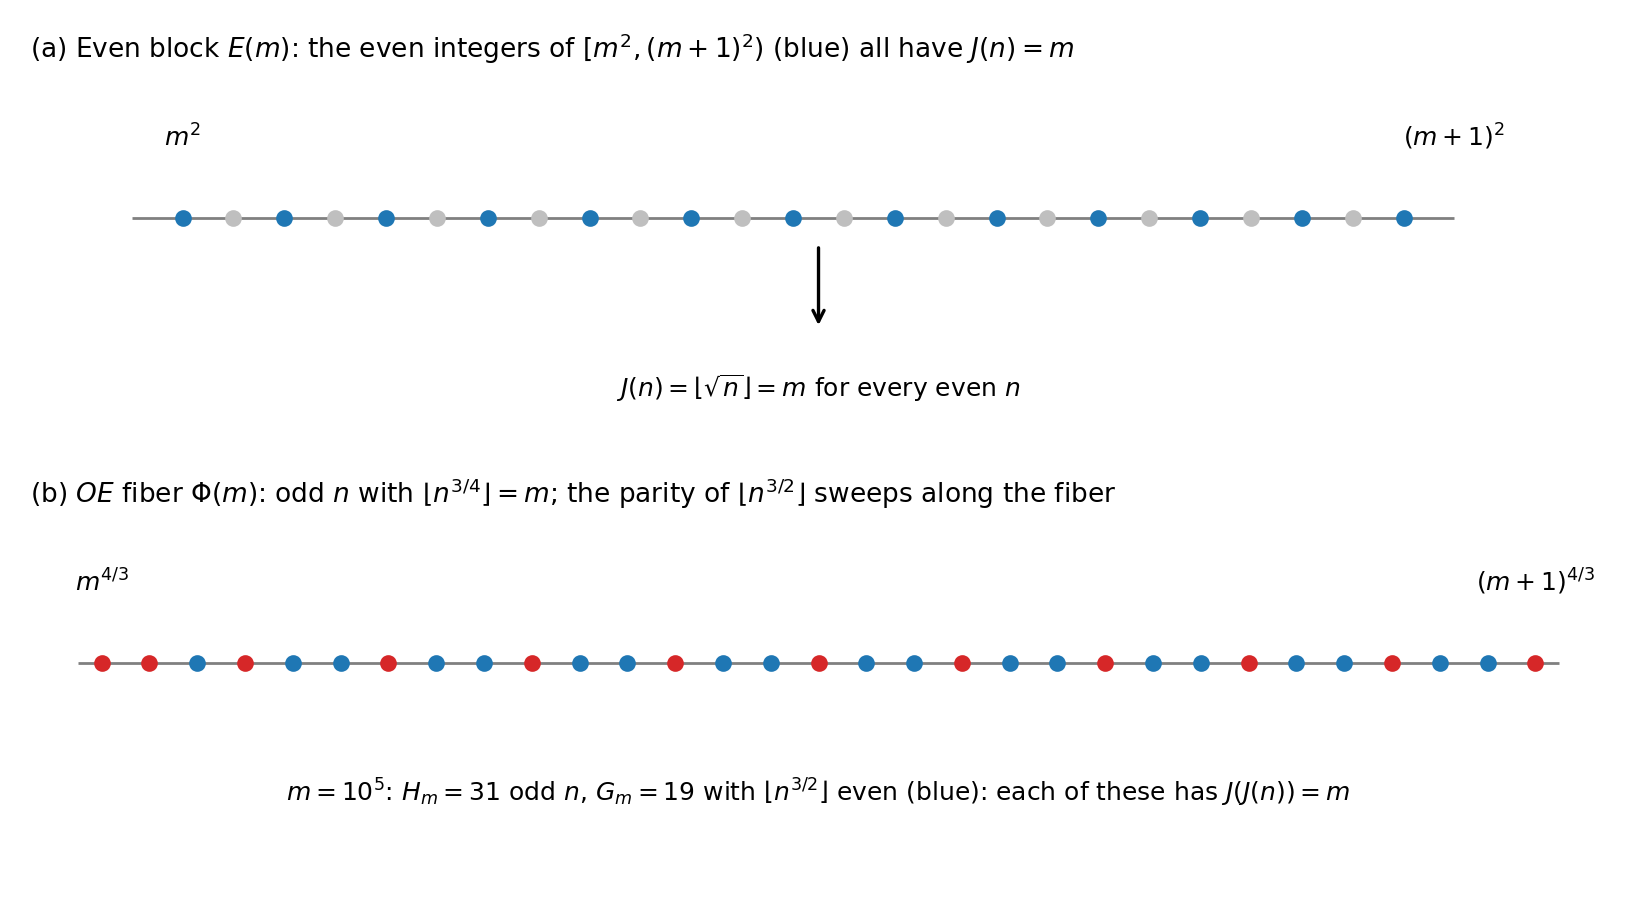
\includegraphics[width=1\linewidth,height=\textheight,keepaspectratio]{figures/paper_c_productions.png}
\caption{The two productions. (a) The even integers of \([m^2,(m+1)^2)\)
all map to \(m\). (b) The \(OE\) fiber \(\Phi(m)\) for \(m=10^5\): the
odd \(n\) with \(\lfloor n^{3/4}\rfloor=m\), coloured by the parity of
\(\lfloor n^{3/2}\rfloor\); those with even image (blue) have
\(J(J(n))=m\).}
\end{figure}

\section{4. Parity on a fiber}\label{parity-on-a-fiber}

\subsection{4.1 The sweep lemma}\label{the-sweep-lemma}

On \(\Phi(m)\) the quantity \(x=n^{3/2}/2\) has
\(\lfloor n^{3/2}\rfloor\) even iff \(\{x\}<\tfrac12\). Consecutive odd
\(n\) advance \(x\) by \(\approx\tfrac32n^{1/2}\approx\tfrac32m^{2/3}\),
and over the whole fiber this step drifts by less than one unit of
\(1/H_m\). So modulo \(1\) the fiber is an arithmetic progression with a
nearly constant step \(\alpha\), of length \(H_m\). Such a progression
cannot avoid a half-circle unless its step is within \(O(1/H_m)\) of
\(0\), or its two-step is (\(\alpha\approx\tfrac12\) with the wrong
phase).

\textbf{Lemma 4.1 (sweep).} Let \(x_1<x_2<\dots<x_H\) be real numbers
with \(x_{j+1}-x_j\in[a,b]\) for all \(j\), where
\(0<a\le b\le\tfrac12\), \(b\le\tfrac{21}{20}a\) and \((H-1)a\ge 12\).
Then \[
\#\{j:\{x_j\}<\tfrac12\}\ \ge\ \tfrac H7
\qquad\text{and}\qquad
\#\{j:\{x_j\}\ge\tfrac12\}\ \ge\ \tfrac H7 .
\] The same holds with the cells \((k/2,(k+1)/2]\) in place of
\([k/2,(k+1)/2)\), i.e.~with the representative in \((0,1]\) in place of
the fractional part.

\emph{Proof.} Cut \(\mathbb R\) into cells \(C_k=[k/2,(k+1)/2)\),
\(k\in\mathbb Z\); even \(k\) are the \emph{good} cells
(\(\{x\}<\tfrac12\)), odd \(k\) the \emph{bad} cells. Call \(C_k\)
\emph{traversed} if \(x_1\le k/2\) and \((k+1)/2\le x_H\).

\begin{enumerate}
\def\labelenumi{(\roman{enumi})}
\item
  \emph{A traversed cell contains at least
  \(g:=\lfloor 1/(2b)\rfloor\ge 1\) and at most
  \(G:=\lfloor 1/(2a)\rfloor+1\) of the points.} Let \(j_0\) be the
  least index with \(x_{j_0}\ge k/2\). Then \(x_{j_0}<k/2+b\) (either
  \(j_0=1\) and \(x_1=k/2\), or \(x_{j_0-1}<k/2\)). Since every step is
  at most \(b\), \(x_{j_0+i}<k/2+(i+1)b\le(k+1)/2\) for all
  \(i\le 1/(2b)-1\), and these indices exist because \((k+1)/2\le x_H\).
  That gives at least \(\lfloor 1/(2b)\rfloor\) points in \(C_k\). Since
  every step is at least \(a\), the points in \(C_k\) are \(x_{j_0+i}\)
  with \(k/2+ia\le x_{j_0+i}<(k+1)/2\), so \(i<1/(2a)\) and there are at
  most \(\lfloor 1/(2a)\rfloor+1\) of them. The same count holds for any
  cell as an upper bound.
\item
  \emph{Counting cells.} The traversed cells are consecutive, and their
  number \(T\) is at least \(2(x_H-x_1)-2\ge 2(H-1)a-2\ge 22\). Good and
  bad traversed cells alternate, so their numbers \(T_g,T_b\) differ by
  at most one and \(T_g,T_b\ge 10\). Every point outside the traversed
  cells lies in the cell of \(x_1\) or the cell of \(x_H\).
\item
  \emph{The ratio.} Hence \(\mathrm{Good}\ge gT_g\) and
  \(H\le G(T_g+T_b+2)\le G(2T_g+3)\), so \[
  \frac{\mathrm{Good}}H\ \ge\ \frac gG\cdot\frac{T_g}{2T_g+3}\ \ge\ \frac gG\cdot\frac{10}{23}.
  \] Put \(X=1/(2a)\ge 1\), so \(G=\lfloor X\rfloor+1\) and, from
  \(b\le\tfrac{21}{20}a\), \(g\ge\lfloor\tfrac{20}{21}X\rfloor\). If
  \(X<2\): \(g\ge 1,G\le 2\). If \(2\le X<3\): \(g\ge 1,G=3\). If
  \(3\le X<4\): \(g\ge 2,G=4\). If \(4\le X<5\): \(g\ge 3,G=5\). If
  \(X\ge 5\): \(g/G\ge(\tfrac{20}{21}X-1)/(X+1)\ge 0.62\). In all cases
  \(g/G\ge\tfrac13\), so \(\mathrm{Good}/H\ge\tfrac{10}{69}>\tfrac17\).
  The bad count is symmetric. For left-open cells the same proof applies
  verbatim (the first point in a cell \((c,c+\tfrac12]\) after a point
  \(\le c\) is \(\le c+b\le c+\tfrac12\)). \(\square\)
\end{enumerate}

Lean: \texttt{\nolinkurl{sweep_fract_lt_half}},
\texttt{\nolinkurl{sweep_fract_ge_half}} (closed cells) and
\texttt{\nolinkurl{sweep_rep_le_half}},
\texttt{\nolinkurl{sweep_rep_gt_half}} (left-open cells, with the
representative \(x-\lceil x\rceil+1\in(0,1]\)), in
\texttt{\nolinkurl{formal/Problems/Juggler/FateSweep.lean}}. The formal
count uses the strictly interior cells (at least \((T-3)/2\) of one
colour, ratio \(11/25\)) in place of the traversed cells (ratio
\(10/23\)), and obtains the left-open case from the closed one by
\(x_j\mapsto -x_{H+1-j}\).

The product \(g/G\cdot 10/23\) cannot reach \(\tfrac13\). An adversarial
sequence with steps in \([a,b]\) can lock a \(3+1\) split near
\(a=\tfrac14\). The OE fiber is monotone.

\textbf{Lemma 4.1' (monotone pairing).} Keep the hypotheses of Lemma 4.1
and assume the consecutive differences are monotone (nondecreasing or
nonincreasing). Then \[
\#\{j:\{x_j\}<\tfrac12\}\ \ge\ \tfrac H3-2
\qquad\text{and}\qquad
\#\{j:\{x_j\}\ge\tfrac12\}\ \ge\ \tfrac H3-2.
\] The same holds with the cells \((k/2,(k+1)/2]\) in place of
\([k/2,(k+1)/2)\).

\emph{Proof.} We prove the nondecreasing case for both half-cell
conventions. Reversing the order and reflecting, \(z_j=-x_{H+1-j}\),
then gives the nonincreasing case; it interchanges the half-cell
conventions and preserves the two color counts up to relabeling. Assume
the steps are nondecreasing. Cut \(\mathbb R\) into the cells
\(C_k=[k/2,(k+1)/2)\) of Lemma 4.1. Since every step is at most
\(b\le\tfrac12\), the cells of \(x_1,\dots,x_H\) are \(T\) consecutive
integers, each visited; write \(\rho_1,\dots,\rho_T\ge 1\) for their
occupancies in order, so \(\sum_i\rho_i=H\), and consecutive cells have
opposite colours. Call the cells \(2,\dots,T-1\) \emph{interior}. Put
\(X=1/(2a)\), \(G=\lfloor X\rfloor+1\) and
\(g=\lfloor 1/(2b)\rfloor\ge 1\). As in Lemma 4.1(i), every cell has
\(\rho_i\le G\) and every interior cell has \(\rho_i\ge g\); and
\((H-1)a\ge 12\) gives \(H\ge 24X+1\ge 24G-23\).

\begin{enumerate}
\def\labelenumi{(\alph{enumi})}
\item
  \emph{A later cell is at most one fuller than an earlier interior
  cell.} Let \(2\le i<j\le T\). The \(\rho_i+1\) steps from the last
  point before the cell of index \(i\) to the first point after it span
  more than \(\tfrac12\), so one of them, \(\gamma\), exceeds
  \(1/(2(\rho_i+1))\). Every step inside the cell of index \(j\) comes
  later, hence is at least \(\gamma\), and the \(\rho_j-1\) steps inside
  that cell span less than \(\tfrac12\). So
  \((\rho_j-1)\gamma<\tfrac12\), i.e.~\(\rho_j\le\rho_i+1\). In
  particular, once an interior cell of occupancy \(v\) has occurred,
  every later cell has occupancy at most \(v+1\).
\item
  \emph{Pairs and surplus.} Pair the interior cells consecutively,
  \((2,3),(4,5),\dots\); at most three cells are unpaired (the first,
  the last, and possibly one interior cell), each holding at most \(G\)
  points. Each pair has one cell of each colour, so each colour receives
  at least \(\sum_{\rm pairs}\min(\rho,\rho')\), and \[
  \sum_{\rm pairs}\min(\rho,\rho')
  \ \ge\ \tfrac13(H-3G)+S,\qquad
  S:=\sum_{\rm pairs}\Bigl(\min(\rho,\rho')-\tfrac{\rho+\rho'}3\Bigr).
  \] It therefore suffices to show \(S\ge G-2\). Both entries of every
  pair lie in \([g,G]\), so every pair has
  \(\min/\mathrm{sum}\ge g/(g+G)=:r\), and a pair contributes at least
  \((r-\tfrac13)(\rho+\rho')\) to \(S\).
\item
  \emph{\(G\ge 7\).} Then \(X\ge 6\) and
  \(g\ge\lfloor\tfrac{20}{21}X\rfloor\) give \(7g\ge 5G\) (\(g\ge 5\) at
  \(G=7\), \(g\ge 6\) at \(G=8\), and \(7g>\tfrac{20G-41}3\ge 5G\) for
  \(G\ge 9\)), so \(r\ge\tfrac5{12}\) and
  \(S\ge\tfrac1{12}(H-3G)\ge\tfrac{21G-23}{12}\ge G-2\).
\item
  \emph{\(3\le G\le 6\) and \(g\ge 2\).} The possible \((G,g)\) are
  \((3,2),(4,2),(4,3),(5,3),(5,4),(6,4),(6,5)\). Except for \((4,2)\),
  \(r\ge\tfrac38\), so
  \(S\ge\tfrac1{24}(H-3G)\ge\tfrac{21G-23}{24}\ge G-2\) because
  \(3G\le 25\). For \((G,g)=(4,2)\) the interior occupancies lie in
  \(\{2,3,4\}\); by (a), after the first interior cell of occupancy
  \(2\) every cell has occupancy at most \(3\). So the pairs with both
  entries in \(\{3,4\}\) (ratio \(\ge\tfrac37\)) precede the pairs with
  both entries in \(\{2,3\}\) (ratio \(\ge\tfrac25\)), and at most one
  pair straddles, with ratio \(\ge\tfrac13\) and at most \(6\) points.
  Hence \(S\ge\tfrac1{15}(H-3G-6)\ge\tfrac{24G-41}{15}>2=G-2\).
\item
  \emph{\(G=2\).} Interior occupancies lie in \(\{1,2\}\), every pair
  has ratio \(\ge\tfrac13\), and \(S\ge 0=G-2\).
\item
  \emph{\(G=3\) and \(g=1\)}, i.e.~\(2\le X<3\) and \(b>\tfrac14\); then
  \(a\le\tfrac14\) and \(b\le\tfrac{21}{80}\), so \(3b<1\) and \(7b<2\).
  Interior occupancies lie in \(\{1,2,3\}\), and by (a) every cell after
  the first interior cell of occupancy \(1\) has occupancy at most
  \(2\). The pairs are therefore: pairs with both entries in
  \(\{2,3\}\), of ratio \(\ge\tfrac25\); at most one straddling pair
  \((\rho,1)\) with \(\rho\in\{2,3\}\), which contributes at least
  \(-\tfrac13\) to \(S\); and pairs with both entries in \(\{1,2\}\). In
  the last group, \((1,1)\) does not occur: two adjacent interior cells
  with one point each would have three consecutive steps spanning more
  than \(1>3b\). Nor do two consecutive pairs with six points in all:
  four consecutive interior cells with six points would have seven
  consecutive steps spanning more than \(2>7b\). So among any two
  consecutive pairs of the last group at least one is \((2,2)\), and the
  two together hold at least \(7\) points of which the scarcer colour
  gets at least \(3\): their contribution to \(S\) is at least
  \(3-\tfrac73=\tfrac23\), and they hold at most \(8\) points, so the
  last group contributes at least \(\tfrac1{12}N_2-\tfrac23\) to \(S\),
  where \(N_2\) is its number of points (a leftover single pair
  contributes at least \(0\)). With \(N_1\) the number of points in the
  first group, \(N_1+N_2\ge H-3G-4=H-13\), and \[
  S\ \ge\ -\tfrac13+\tfrac1{15}N_1+\tfrac1{12}N_2-\tfrac23
  \ \ge\ \tfrac1{15}(H-13)-1\ \ge\ 1=G-2,
  \] since \(H\ge 24X+1\ge 49\).
\end{enumerate}

In all cases \(S\ge G-2\), so the scarcer colour has at least
\(\tfrac13(H-3G)+G-2=\tfrac H3-2\) points. For left-open cells the same
argument applies with the cells \((k/2,(k+1)/2]\), or apply the closed
case to \(-x_{H+1-j}\) as in Lemma 4.1. \(\square\)

Lean: \texttt{\nolinkurl{sweep_monotone_fract_lt_half}},
\texttt{\nolinkurl{sweep_monotone_fract_ge_half}} (closed cells) and
\texttt{\nolinkurl{sweep_monotone_rep_le_half}},
\texttt{\nolinkurl{sweep_monotone_rep_gt_half}} (left-open cells),
instances of \texttt{\nolinkurl{Sweep.sweep_monotone_cell}} and
\texttt{\nolinkurl{sweep_monotone_ceil}}, in
\texttt{\nolinkurl{formal/Problems/Juggler/FateSweepMonotone.lean}}.

\emph{Remark (erratum, 8 September 2026).} An earlier version of this
proof asserted that every pair satisfies \(\min\ge(\rho+\rho')/3\), on
the grounds that the step scale \(1/(2\delta)\) changes by at most
\(X/21\) ``spread over the cells'' and that with \(X<2.1\) the pairs are
\((1,1)\), \((1,2)\) or \((2,2)\). Monotone steps need not change
gradually: with \(a=\tfrac{10}{41}\), \(b=\tfrac{21}{82}\) the sequence
\(-2a,-a,0,a,2a,2a+b,2a+2b,\dots\) has nondecreasing steps in \([a,b]\),
and its cells \(2\) and \(3\) --- an interior pair in the pairing of (b)
--- have occupancies \((3,1)\). That version also paired the two partial
end cells as if they were interior. The statement is unchanged; the
proof above replaces it, with (a) in place of the spreading claim, the
end cells left unpaired, and the surplus \(S\) paying for them.

\textbf{Lemma 4.2 (fiber parity).} For \(m\ge 10^6\) put
\(\alpha_m=\{\tfrac32m^{2/3}\}\) and call \(m\) \emph{good} if \[
\|\alpha_m\|\ \ge\ 22\,m^{-1/3}
\qquad\text{and}\qquad
\|\alpha_m-\tfrac12\|\ \ge\ 2\,m^{-1/3},
\] where \(\|\cdot\|\) is the distance to the nearest integer. If \(m\)
is good then \(G_m\ge\tfrac13H_m-2\) and \(H_m-G_m\ge\tfrac13H_m-2\).

\emph{Proof.} Let \(n_1<\dots<n_H\) be the odd integers of \(\Phi(m)\),
\(n_{j+1}=n_j+2\), and \(x_j=n_j^{3/2}/2\). Then
\(\lfloor n_j^{3/2}\rfloor\) is even iff \(\{x_j\}<\tfrac12\). The steps
are \[
\delta_j=x_{j+1}-x_j=\int_{n_j}^{n_j+2}\tfrac34t^{1/2}\,dt
\in\bigl[\tfrac32n_j^{1/2},\ \tfrac32(n_j+2)^{1/2}\bigr]
\subseteq[A_m,B_m],
\] with \(A_m=\tfrac32m^{2/3}\) and
\(B_m=\tfrac32\bigl((m+1)^{4/3}+2\bigr)^{1/2}\). Using
\(\sqrt u-\sqrt v\le(u-v)/(2\sqrt v)\) and
\((m+1)^{4/3}-m^{4/3}\le\tfrac43(m+1)^{1/3}\), \[
\eta_m:=B_m-A_m\le\frac{(m+1)^{1/3}+\tfrac32}{m^{2/3}}
\le m^{-1/3}\Bigl(1+\frac1{3m}+\frac32m^{-1/3}\Bigr)\le 1.02\,m^{-1/3}.
\] Also \(H_m-1\ge\tfrac23m^{1/3}-2\ge 0.646\,m^{1/3}\).

\emph{Case 1: \(\alpha_m\le\tfrac12-2m^{-1/3}\).} Put
\(N=\lfloor A_m\rfloor\) and \(y_j=x_j-jN\); then \(\{y_j\}=\{x_j\}\)
and the steps of \(y\) lie in
\([a,b]=[\alpha_m,\alpha_m+\eta_m]\subseteq[22m^{-1/3},\tfrac12]\). Now
\(b/a\le 1+1.02/22<\tfrac{21}{20}\) and \((H-1)a\ge 0.646\cdot 22>12\).
The steps of \(y\) are nondecreasing. Lemma 4.1' applies.

\emph{Case 2: \(\alpha_m\ge\tfrac12+2m^{-1/3}\).} Put
\(z_j=j(N+1)-x_j\), increasing with steps
\((N+1)-\delta_j\in[1-\alpha_m-\eta_m,\ 1-\alpha_m]\subseteq[20.98\,m^{-1/3},\ \tfrac12]\);
again \(b/a\le 1+1.02/20.98<\tfrac{21}{20}\) and
\((H-1)a\ge 0.646\cdot 20.98>12\). Write \(\langle z\rangle\in(0,1]\)
for the representative of \(z\) modulo \(1\) in \((0,1]\). Then
\(\langle z_j\rangle=1-\{x_j\}\) for every \(j\), so
\(\{x_j\}<\tfrac12\iff\langle z_j\rangle\in(\tfrac12,1]\). The steps of
\(z\) are monotone. Lemma 4.1' in its left-open form gives both counts.

The middle range \(|\alpha_m-\tfrac12|<2m^{-1/3}\) and the range
\(\|\alpha_m\|<22m^{-1/3}\) are excluded by goodness. \(\square\)

\textbf{Lemma 4.3 (bad fibers are thin).} For \(u\ge 10^6\), \[
\#\{m\in(u,2u]:\ m\ \text{bad}\}\le 63\,u^{2/3},
\qquad
\sum_{\substack{m>U\\ m\ \text{bad}}}\frac1m\le 306\,U^{-1/3}\quad(U\ge 10^6).
\]

\emph{Proof.} \(\varphi(m)=\tfrac32m^{2/3}\) increases with
\(\varphi(m+1)-\varphi(m)\in[(m+1)^{-1/3},m^{-1/3}]\subseteq[(3u)^{-1/3},u^{-1/3}]\)
on \((u,2u]\). Badness means \(\{\varphi(m)\}\) lies in one of two arcs
of the circle, of total length at most \(48\,u^{-1/3}\). As \(m\) runs
over \((u,2u]\), \(\varphi\) increases by
\(\tfrac32u^{2/3}(2^{2/3}-1)<0.882\,u^{2/3}\), so it passes each arc at
most \(0.882u^{2/3}+2\) times, and each pass through an arc of length
\(w\) takes at most \(w(3u)^{1/3}+1\) values of \(m\). Hence the count
is at most \((0.882u^{2/3}+2)(48\cdot 3^{1/3}+2)\le 63\,u^{2/3}\) for
\(u\ge 10^6\). Summing \(63\,(2^iU)^{-1/3}\) over \(i\ge 0\) gives
\(63U^{-1/3}/(1-2^{-1/3})\le 306\,U^{-1/3}\). \(\square\)

\subsection{4.2 The block average}\label{the-block-average}

The adversarial sweep \(G_m\ge H_m/7\) is not the fiber bound: Lemma
4.1' gives the monotone floor \(H_m/3-2\). In the numerical experiments
of Section 11 the mean of \(G_m/H_m\) is \(\tfrac12\) and the minimum on
good fibers is near \(\tfrac13\). When the members of \(A\) come in even
blocks --- as the \(E\)-produced part of \(A\) always does --- the
fibers can be averaged over the block, and the average is asymptotically
\(\tfrac12\) by a classical exponential-sum estimate.

\textbf{Proposition 4.4 (block average).} For \(m'\ge2\), put
\(I(m')=[m'^{8/3},(m'+1)^{8/3})\) and \[
U(m')=\{n\text{ odd in }I(m'):
 \lfloor n^{3/4}\rfloor\text{ even},\quad
 \lfloor n^{3/2}\rfloor\text{ even}\}.
\] This is the disjoint union of the even-image parts of \(\Phi(m)\)
over \(m\in E(m')\). There is an absolute constant \(C_B\) such that \[
\left||U(m')|-\tfrac14\#\{n\text{ odd in }I(m')\}\right|
 \le C_B m'^{11/9}\log(m'+1).
\tag{4.1}
\] In particular \[
|U(m')|=\tfrac13m'^{5/3}(1+O(m'^{-4/9}\log(m'+1))).
\] No numerical value of \(C_B\) is asserted.

\emph{Proof.} Write \(M=\#\{n\text{ odd in }I(m')\}\asymp m'^{5/3}\) and
\(\psi(z)=(-1)^{\lfloor z\rfloor}\). Expanding the two indicators gives
four sums: \(M\), the sums of \(\psi(n^{3/4})\) and \(\psi(n^{3/2})\),
and their product.

The slow sum is \(O(m')\): pair consecutive fibers of
\(\lfloor n^{3/4}\rfloor\), whose odd-point counts differ by at most
\(3\), and bound the remaining end fiber by \(O(m'^{2/3})\).

We use the interval form of Vaaler's approximation {[}10{]}. For
\(J\ge1\), the parity wave has a trigonometric approximation
\(V_J(z/2)\), with zero constant term and coefficients \(O(1/|q|)\), and
a nonnegative error majorant \(\Delta_J(z/2)\). Its degree is \(J\),
every coefficient is \(O(1/J)\), and \(\|\Delta_J\|_\infty=O(1)\). All
constants in this paragraph are absolute; the interval endpoints are
included in the majorant.

Take \(J=\max(1,\lfloor m'^{4/9}\rfloor)\) and reindex odd integers as
\(n=2r+1\). For \(q\ne0\), the fast phase \(f(r)=q(2r+1)^{3/2}/2\) has
\(|f''|\asymp |q|m'^{-4/3}\), with constant sign. The second-derivative
test {[}13, Theorem 2.2{]} gives, uniformly on initial subintervals, \[
\left|\sum_r e(f(r))\right|
 \ll m'|q|^{1/2}+m'^{2/3}|q|^{-1/2},\qquad e(z)=e^{2\pi iz}.
\] The coefficient sum and the majorant sum are therefore bounded by \[
\ll m'J^{1/2}+m'^{2/3}+M/J\ll m'^{11/9}.
\] For the product, expand both waves. A mixed phase is
\(f=(q_1n^{3/4}+q_2n^{3/2})/2\), with \(q_2\ne0\), and \[
f''(r)=\tfrac32q_2n^{-1/2}
 \left(1-\frac{q_1}{4q_2}n^{-3/4}\right).
\] For \(|q_1|\le J\), the correction is \(O(m'^{-14/9})\); for all
sufficiently large \(m'\) the same second-derivative estimate applies
uniformly. Summing the slow coefficients adds at most \(O(\log(J+1))\).

The slow majorant has constant contribution \(O(M/J)\). Its nonzero
modes have monotone derivative \(\tfrac34 q_1 n^{-1/4}\), of magnitude
\(\asymp |q_1|m'^{-2/3}\) and at most \(1/2\) for sufficiently large
\(m'\). Kusmin--Landau {[}13, Theorem 2.1{]} bounds a mode by
\(O(m'^{2/3}/|q_1|)\), so the majorant contributes
\(O(M/J+m'^{2/3}\log(J+1)/J)\). Since \(|\psi|=1\),
\(|V_J|\le1+\Delta_J=O(1)\), and the majorants are nonnegative, the
product-approximation error is bounded by a constant times the sum of
the two majorants. These estimates prove (4.1) for sufficiently large
\(m'\); increasing the unspecified absolute constant covers the finitely
many smaller integers \(m'\ge2\). \(\square\)

\emph{Revision note.} The earlier value \(C_0=250\) depended on an
unverified explicit majorant and small-parameter inequalities that do
not hold throughout their printed range. The asymptotic form above is
all that the subsequent recursions use.

\subsection{4.3 The share is a quadratic
sweep}\label{the-share-is-a-quadratic-sweep}

Sections 4.1 and 4.2 bound \(G_m\) from below, by a sweep on each good
fiber and by an exponential sum across an even block. Neither says what
\(G_m/H_m\) \emph{is}. It has a closed form, and the form explains both
the floor of Lemma 4.2 and the extreme fibers that the goodness
condition excludes. Nothing in Sections 5--10 depends on this
subsection; it is here because it identifies which of the two tools is
doing the work, and because it names the hypothesis behind the gap
between them.

Throughout, \(n_1=\min\Phi(m)\), \(n_j=n_1+2(j-1)\), and
\(x_j=n_j^{3/2}/2\), so that \(\lfloor n_j^{3/2}\rfloor\) is even iff
\(\{x_j\}<\tfrac12\). Write \[
\theta_m=\{x_1\},\qquad
\beta_m=\alpha_m\,(H_m-1),
\] with \(\alpha_m=\{\tfrac32m^{2/3}\}\) as in Lemma 4.2, taken in
\((-\tfrac12,\tfrac12]\), and set \[
S(\beta,\theta)
=\bigl|\{s\in[0,1]:\ \{\theta+\beta s+\tfrac13s^2\}<\tfrac12\}\bigr|.
\]

\textbf{Lemma 4.5 (share law).} As \(m\to\infty\), \[
G_m/H_m=S(\beta_m,\theta_m)
 +O\left(H_m^{-1/2}+\frac{1+|\beta_m|}{H_m}\right).
\] The estimate is useful when \(|\beta_m|=o(H_m)\); it is not a uniform
equidistribution assertion for all fibers.

\emph{Proof.} Expand \(x_j\) about \(n_1\). With \(u=2(j-1)/n_1\), \[
x_j=\tfrac12n_1^{3/2}(1+u)^{3/2}
=x_1+\tfrac32n_1^{1/2}(j-1)+\tfrac34n_1^{-1/2}(j-1)^2+E_j,
\qquad |E_j|\le\tfrac14(j-1)^3n_1^{-3/2}.
\] On the fiber \(j-1\le H_m-1\ll m^{1/3}\) and \(n_1\ge m^{4/3}\), so
\(|E_j|\ll m^{-1}\), below \(1/H_m\). Put \(s=(j-1)/(H_m-1)\in[0,1]\).
The linear coefficient is \(A=\tfrac32n_1^{1/2}\), and since
\(n_1=m^{4/3}+O(1)\) we have \(A=\tfrac32m^{2/3}+O(m^{-2/3})\), so
\(A\equiv\alpha_m+O(m^{-2/3})\pmod1\) and the accumulated difference
over the fiber is \(O(m^{-1/3})=O(1/H_m)\). Hence
\(A(j-1)\equiv\beta_ms\pmod 1\) up to \(O(1/H_m)\). The quadratic
coefficient gives \(\tfrac34n_1^{-1/2}(H_m-1)^2=\tfrac13+O(1/H_m)\) by
Lemma 3.2, so \[
x_j\ \equiv\ \theta_m+\beta_ms+\tfrac13s^2\pmod 1,
\] uniformly to \(O(1/H_m)\). Put \(\epsilon=O(1/H_m)\). Replacing the
exact phase by the displayed quadratic can change an indicator only
within \(\epsilon\) of an integer or half-integer. If \(|\beta_m|\le2\),
there are \(O(1)\) such levels and their inverse images have total
length \(O(\sqrt\epsilon)\), since the quadratic has second derivative
\(2/3\). If \(|\beta_m|>2\), its derivative has magnitude at least
\(|\beta_m|-2/3\), and the total inverse-image length is
\(O(\epsilon)\). Each of these sets, and each half-cell inverse image,
has \(O(1+|\beta_m|)\) interval components. Sampling on the uniform grid
costs \(O((1+|\beta_m|)/H_m)\). This proves the stated bound, including
tangencies to the cell boundaries. \(\square\)

\textbf{Corollary 4.6.} For every \(\beta\):

\begin{enumerate}
\def\labelenumi{\arabic{enumi}.}
\tightlist
\item
  \(\int_0^1S(\beta,\theta)\,d\theta=\tfrac12\).
\item
  \(S(\beta,\theta)\in\{0,1\}\) for some \(\theta\) if and only if
  \(\beta\in[-\tfrac56,\tfrac16]\).
\item
  \(\displaystyle\int\bigl|\{\theta:S(\beta,\theta)=0\}\bigr|\,d\beta=\tfrac{25}{108}\),
  and the same for \(S=1\).
\end{enumerate}

\emph{Proof.} (1) By Fubini the integral is
\(\int_0^1\!\int_0^1\mathbf 1[\{\theta+\varphi(s)\}<\tfrac12]\,d\theta\,ds\),
and the inner integral is \(\tfrac12\) for every \(s\), whatever
\(\varphi\).

\begin{enumerate}
\def\labelenumi{(\arabic{enumi})}
\setcounter{enumi}{1}
\item
  Let \(\varphi(s)=\beta s+\tfrac13s^2\), so
  \(\varphi'(s)=\beta+\tfrac23s\). If \(\beta\ge0\) then \(\varphi\) is
  increasing with range \(\beta+\tfrac13\); if \(\beta\le-\tfrac23\) it
  is decreasing with range \(-\beta-\tfrac13\); and if
  \(-\tfrac23<\beta<0\) it dips to
  \(\varphi(-\tfrac32\beta)=-\tfrac34\beta^2\) and returns to
  \(\beta+\tfrac13\), so its range is
  \(\max(0,\beta+\tfrac13)+\tfrac34\beta^2\). An extreme value of \(S\)
  needs the image of \([0,1]\) to miss a half-circle, hence range
  \(\le\tfrac12\). That is \(\beta\le\tfrac16\) in the first case,
  \(\beta\ge-\tfrac56\) in the second, and no constraint in the third,
  since the range there is at most \(\tfrac13\).
\item
  The \(\theta\)-measure is \(\max(0,\tfrac12-\text{range})\).
  Integrating the four pieces of (2), \[
  \int_0^{1/6}\!\!\bigl(\tfrac16-\beta\bigr)
  +\int_{-1/3}^0\!\!\bigl(\tfrac16-\beta-\tfrac34\beta^2\bigr)
  +\int_{-2/3}^{-1/3}\!\!\bigl(\tfrac12-\tfrac34\beta^2\bigr)
  +\int_{-5/6}^{-2/3}\!\!\bigl(\tfrac56+\beta\bigr)
  =\tfrac1{72}+\tfrac{11}{108}+\tfrac{11}{108}+\tfrac1{72}
  =\tfrac{25}{108}.
  \] The statement for \(S=1\) is the reflection
  \(\theta\mapsto\theta+\tfrac12\). \(\square\)
\end{enumerate}

Part (1) is the reason no aggregate count in this paper sees the extreme
fibers: they are compensated at every drift separately, which is what
Proposition 4.4 recovers by a different route. Part (2) says the
extremes occupy a window of one drift unit, that is
\(\alpha_m\in[-\tfrac54,\tfrac14]m^{-1/3}\) by
\(H_m\sim\tfrac23m^{1/3}\).

At the centre of that window the law degenerates to an identity.

\textbf{Lemma 4.7 (cube fibers).} Let \(k\ge2\) and \(m=k^3\). Every
\(n\in\Phi(m)\) has \(n=k^4+t\) with \(3t\le4k\), and then
\(\lfloor n^{3/2}\rfloor=k^6+\tfrac32k^2t\) exactly. Consequently the
fiber of an even cube is full, \(G_m=H_m\), and along the fiber of an
odd cube the images alternate in parity, so \(|2G_m-H_m|\le1\).

\emph{Proof.} If \(3t\ge4k+1\) then
\((3k^4+4k+1)^3\le(3k^4+3t)^3=27(k^4+t)^3\), and
\((3k^4+4k+1)^3\ge27(k^3+1)^4\), so \(n^3\ge(k^3+1)^4\) and
\(n\notin\Phi(m)\). Given \(3t\le4k\), the claimed value
\(q=k^6+\tfrac32k^2t\) satisfies \(n^3-q^2=\tfrac34k^4t^2+t^3\ge0\) and
\((q+1)^2-n^3=2k^6+3k^2t+1-\tfrac34k^4t^2-t^3>0\), so
\(q=\lfloor n^{3/2}\rfloor\). For even \(k\) the value
\(k^6+\tfrac32k^2t\) is even for every \(t\); for odd \(k\) the fiber's
\(t\) are even and the value has the parity of \(1+t/2\). Lean:
\texttt{\nolinkurl{cube_fiber_range}},
\texttt{\nolinkurl{cube_fiber_sqrt_even}},
\texttt{\nolinkurl{cube_fiber_sqrt_odd}},
\texttt{\nolinkurl{even_cube_fiber_full}},
\texttt{\nolinkurl{odd_cube_fiber_alternating}} in
\texttt{\nolinkurl{formal/Problems/Juggler/CubeFiber.lean}}. \(\square\)

\textbf{Remark 4.8 (what the window is, arithmetically).} \(\alpha_m=0\)
exactly means \(\tfrac32m^{2/3}\in\mathbb Z\), that is \(27m^2=8k^3\),
whose integer solutions are \(m=(2e)^3\) and \(k=6e^2\). So the centre
of the extreme window is the even cubes of Lemma 4.7, and the window
itself is the near-solution set of that equation; the crossings are
spaced \(\asymp m^{1/3}\) apart, giving \(\sim\tfrac32M^{2/3}\) of them
below \(M\). Two consequences worth recording. The set is asymmetric
about \(0\), which the symmetric goodness condition of Lemma 4.2 cannot
express: that condition discards \(\|\alpha_m\|<22m^{-1/3}\), of width
\(44m^{-1/3}\), against the \(\tfrac32m^{-1/3}\) the extremes actually
occupy. Nothing here depends on the difference, since Lemma 4.3 already
makes the discarded mass \(o(1)\); the point is that the goodness
threshold is a convenience, not a boundary of the phenomenon. And the
two sides of the window are not symmetric in strength either: full
fibers contain the infinite family of Lemma 4.7, proved, whereas an
empty fiber requires a near-miss together with a phase condition, and
whether there are infinitely many is open.

\textbf{Remark 4.9 (averaging the rest term).} Item 3 of Section 5.1 has
coefficient \(2/9\); a weighted mean even-image share of \(1/2+o(1)\) on
that source set would give \(1/3\). Such a weighted mean is a sufficient
additional hypothesis. Conditional equidistribution of the landing
phases could help establish it if the approximation errors and the
weights were also controlled, but equidistribution is not necessary for
one mean identity. Neither Corollary 4.6(1), which averages an
independent model phase, nor a pointwise bound on each fiber establishes
the required average on an arbitrary backward-closed set. The goodness
condition already removes its exceptional fibers at total logarithmic
cost \(o(1)\).

\section{5. The recursion and the contagion
theorem}\label{the-recursion-and-the-contagion-theorem}

\subsection{\texorpdfstring{5.1 Three sources of members of \(A\) in
\((\sqrt x,x]\)}{5.1 Three sources of members of A in (\textbackslash sqrt x,x{]}}}\label{three-sources-of-members-of-a-in-sqrt-xx}

Let \(x\ge 2\) and \(t=\log x\). Three families of members of
\(A\cap(\sqrt x,x]\) are pairwise disjoint.

\begin{enumerate}
\def\labelenumi{\arabic{enumi}.}
\item
  \textbf{\(E\)-images.} For \(m\in A\cap(x^{1/4},\sqrt x-1]\),
  \(E(m)\subseteq(\sqrt x,x]\) (as \(m^2>\sqrt x\) and
  \((m+1)^2\le x\)). Distinct \(m\) give disjoint blocks. By Lemma 3.1
  the log-mass is at least
  \(\sum_m\frac1m(1-\frac2m)\ge(1-2x^{-1/4})\,\ell_A(x^{1/4},\sqrt x-1]\),
  and \(\ell_A(x^{1/4},\sqrt x-1]\ge g_A(t/2)-2x^{-1/2}\) (at most one
  integer lies in \((\sqrt x-1,\sqrt x]\)).
\item
  \textbf{\(OE\)-images of \(E\)-blocks.} For
  \(m'\in A\cap(x^{3/16},x^{3/8}-1]\),
  \(U(m')\subseteq A\cap(\sqrt x,x]\) (Lemma 3.2 applied to the even
  \(m\in E(m')\subseteq A\); \(I(m')\subseteq(\sqrt x,x]\) as
  \(m'^{8/3}>\sqrt x\) and \((m'+1)^{8/3}\le x\)). Distinct \(m'\) give
  disjoint \(I(m')\). Each \(n\in U(m')\) has \(1/n>(m'+1)^{-8/3}\), so
  by Proposition 4.4 the log-mass of \(U(m')\) is at least
  \(\tfrac13m'^{5/3}(1-\varepsilon_B(m'))(m'+1)^{-8/3}\ge\frac1{3m'}\bigl(1-\varepsilon_B(m')-\tfrac8{3m'}\bigr)\),
  and summing,
  \(\ge\tfrac13(1-\varepsilon'(x))\bigl(g_A(3t/8)-2x^{-3/8}\bigr)\) with
  \(\varepsilon_B(m')=O(m'^{-4/9}\log(m'+1))\ge0\) chosen to bound the
  error in Proposition 4.4 and
  \(\varepsilon'(x)=\sup_{m'>x^{3/16}}(\varepsilon_B(m')+\tfrac8{3m'})\to0\).
\item
  \textbf{\(OE\)-images of the rest.} Let
  \(A^{E}_x=\bigcup_{m''\in A}E(m'')\cap(x^{3/8},x^{3/4}]\) be the
  \(E\)-produced part of \(A\cap(x^{3/8},x^{3/4}]\) and
  \(A^{\rm rest}_x\) its complement in \(A\cap(x^{3/8},x^{3/4}]\). The
  blocks meeting \((x^{3/8},x^{3/4}]\) come from
  \(m''\in[x^{3/16}-1,x^{3/8}]\), so
  \(\ell(A^E_x)\le\sum_{m''}\frac{m''+1}{m''^2}\le(1+2x^{-3/16})\bigl(g_A(3t/8)+2x^{-3/16}\bigr)\)
  and
  \(\ell(A^{\rm rest}_x)\ge g_A(3t/4)-(1+2x^{-3/16})\bigl(g_A(3t/8)+2x^{-3/16}\bigr)\).
  For \(m\in A^{\rm rest}_x\) with \(m\le x^{3/4}-1\) (this drops at
  most one element, of log-mass \(\le 2x^{-3/4}\)),
  \(\Phi(m)\subseteq(\sqrt x,x]\); the fibers are disjoint from each
  other and from those of item 2 (different \(m\)), and for good
  \(m\ge 10^6\) Lemmas 4.2 and 3.2 give log-mass at least
  \(\bigl(\tfrac13H_m-2\bigr)(m+1)^{-4/3}\ge\frac2{9m}\bigl(1-O(m^{-1/3})\bigr)\).
  Bad \(m>x^{3/8}\) carry log-mass at most \(306x^{-1/8}\) (Lemma 4.3).
  Hence item 3 contributes at least
  \(\tfrac2{9}(1-O(x^{-1/8}))\bigl[\ell(A^{\rm rest}_x)-306x^{-1/8}-2x^{-3/4}\bigr]_+\).
\end{enumerate}

The images in item 1 are even, those in items 2--3 odd, so the three
families are disjoint, and all lie in \((\sqrt x,x]\).

\subsection{5.2 The functional
inequalities}\label{the-functional-inequalities}

Adding items 1 and 2: \[
g_A(t)\ \ge\ (1-\varepsilon_1(t))\,g_A(t/2)+\tfrac13(1-\varepsilon_2(t))\,g_A(3t/8)-\varepsilon_3(t),
\tag{5.1}
\] with \(\varepsilon_1=2e^{-t/4}\),
\(\varepsilon_2=\varepsilon'(e^t)\),
\(\varepsilon_3=2e^{-t/2}+e^{-3t/8}\), all tending to \(0\). Adding item
3 as well, and noting that the coefficient of the \emph{actual} value
\(g_A(3t/8)\) is
\(\tfrac13(1-\varepsilon_2)-\tfrac2{9}(1+2e^{-3t/16})\to\tfrac19>0\): \[
g_A(t)\ \ge\ (1-\varepsilon_1)\,g_A(t/2)+\bigl(\tfrac19-\varepsilon_4\bigr)g_A(3t/8)+\bigl(\tfrac29-\varepsilon_5\bigr)g_A(3t/4)-\varepsilon_6(t),
\tag{5.2}
\] with \(\varepsilon_4,\varepsilon_5,\varepsilon_6\to 0\) (for \(t\) so
large that \(x^{3/8}\ge 10^6\); the bracket \([\cdot]_+\) may be dropped
because the right side of (5.2) is a lower bound for it). Every
coefficient of a \(g_A\)-value on the right is nonnegative for large
\(t\), so lower bounds for \(g_A\) at \(t/2\), \(3t/8\), \(3t/4\)
transfer.

\subsection{5.3 The recursion lemma}\label{the-recursion-lemma}

The passage from a functional inequality with vanishing errors to a
power lower bound is a standalone statement.

\textbf{Lemma 5.1 (recursion lemma).} Let \(e_1,\dots,e_r\in(0,1)\),
\(c_1,\dots,c_r\ge 0\), and \(\lambda\in(0,1)\) with \[
\zeta:=\sum_{i=1}^rc_ie_i^{\lambda}-1>0 .
\] Put \(e_{\min}=\min_ie_i\), \(e_{\max}=\max_ie_i\). Let
\(g:(0,\infty)\to[0,\infty)\) satisfy, for all \(t\ge t_1\), \[
g(t)\ \ge\ \sum_{i=1}^r\bigl(c_i-\eta_i(t)\bigr)\,g(e_it)-\eta_0(t),
\] where \(0\le\eta_i(t)\le c_i\) for \(i\ge 1\), \(\eta_0(t)\ge 0\),
and \(\sum_{i\ge1}\eta_i(t)e_i^\lambda\le\zeta/3\) and
\(\eta_0(t)\le\tfrac{2\zeta}3c_0\) for all \(t\ge t_1\), for some
\(c_0>0\) with \(g(t)\ge c_0\) on \([e_{\min}t_1,\,t_1]\). Then \[
g(t)\ \ge\ K\,t^{\lambda}\quad\text{for all }t\ge e_{\min}t_1,\qquad K=c_0t_1^{-\lambda}.
\]

\emph{Proof.} On \([e_{\min}t_1,t_1]\),
\(Kt^\lambda\le Kt_1^\lambda=c_0\le g(t)\). Suppose
\(g(t)\ge Kt^\lambda\) holds on \([e_{\min}t_1,T]\) for some
\(T\ge t_1\), and let \(t\in(T,T/e_{\max}]\). Then
\(e_it\le e_{\max}t\le T\) and \(e_it\ge e_{\min}t>e_{\min}t_1\), so
each \(e_it\) lies in the interval where the bound is known, and
\(t\ge t_1\), so \[
\begin{aligned}
g(t)&\ge\sum_i(c_i-\eta_i(t))K(e_it)^\lambda-\eta_0(t)\\
&=Kt^\lambda\left[\sum_i c_i e_i^\lambda-\sum_i\eta_i(t)e_i^\lambda\right]-\eta_0(t)\\
&\ge Kt^\lambda\left(1+\frac{2\zeta}3\right)-\frac{2\zeta}3c_0
\ge Kt^\lambda.
\end{aligned}
\] using \(c_0=Kt_1^\lambda\le Kt^\lambda\). Hence the bound holds on
\([e_{\min}t_1,T/e_{\max}]\); induction on \(N\) covers
\([e_{\min}t_1,t_1e_{\max}^{-N}]\) for every \(N\), i.e.~all
\(t\ge e_{\min}t_1\). \(\square\)

Lean: \texttt{\nolinkurl{recursion_lemma}} in
\texttt{\nolinkurl{formal/Problems/Juggler/FateRecursion.lean}}, with
\(e_{\min}\le e_i\le e_{\max}\) as bounds rather than extrema and
\(\lambda>0\) in place of \(\lambda\in(0,1)\); the hypotheses \(g\ge 0\)
and \(\lambda<1\) are not used.

\subsection{5.4 The seed}\label{the-seed}

\textbf{Lemma 5.2 (seed).} Every nonempty backward-closed \(A\) contains
an integer \(m\ge 3\), and for any such \(m\), \[
g_A(t)\ \ge\ c_A:=\Bigl(1-\frac2{m^4}\Bigr)\Bigl(\frac{0.375}{m+1}-\frac1{(m+1)^2-1}\Bigr)>0
\qquad\text{for all}\ t\ge 4\log(m+1).
\]

\emph{Proof.} If \(A\ni a\le 2\) then \(E(a)\subseteq A\) contains \(2\)
or \(4\), and \(E(2)\ni 4\), so \(A\ni 4\). Fix \(m\ge 3\) in \(A\) and
let \(S_1=E(m)\), \(S_{k+1}=\bigcup_{m''\in S_k}E(m'')\). Then
\(S_k\subseteq A\cap[m^{2^k},(m+1)^{2^k})\) and, by Lemma 3.1,
\(\ell(S_{k+1})\ge(1-2m^{-2^k})\ell(S_k)\), so
\(\ell(S_k)\ge\ell(S_1)\prod_{j\ge 1}(1-2m^{-2^j})\ge 0.75\,\ell(S_1)\ge\frac{0.375}{m+1}\)
for \(m\ge 3\). Let \(y\ge(m+1)^4\) and choose \(k\ge 2\) with
\((m+1)^{2^k}\le y<(m+1)^{2^{k+1}}\). Then \(S_k\subseteq(y^{1/4},y]\)
(as \(y<m^{2^{k+2}}\)). The members of \(S_k\) above \(\sqrt y\) lie in
\((\sqrt y,y]\); the members in \((y^{1/4},\sqrt y-1]\) have their
\(E\)-images in \((\sqrt y,y]\), with log-mass at least
\((1-2m^{-2^k})\) times their own; at most one member lies in
\((\sqrt y-1,\sqrt y]\), with \(1/n\le 1/((m+1)^2-1)\). Hence
\(g_A(\log y)\ge(1-2m^{-4})\bigl(\ell(S_k)-1/((m+1)^2-1)\bigr)\ge c_A\),
and \(c_A>0\) because \(0.375(m+1)\ge 1+0.375/(m+1)\) for \(m\ge 3\).
\(\square\)

\subsection{5.5 The theorem}\label{the-theorem}

Let \(\lambda^*\) be the root in \((0,1)\) of
\(2^{-\lambda}+\tfrac13(\tfrac38)^{\lambda}=1\), let
\(\lambda_{\mathrm{pair}}\) be the pairing-only root of
\(2^{-\lambda}+\tfrac19(\tfrac38)^{\lambda}+\tfrac29(\tfrac34)^{\lambda}=1\),
and let \(\lambda^{**}\) be the root of (1.1). All three defining sums
are continuous and strictly decreasing on \([0,1]\), with value greater
than \(1\) at \(0\) and less than \(1\) at \(1\); each therefore has a
unique root there. Numerically \(\lambda^*\approx0.3774\),
\(\lambda_{\mathrm{pair}}\approx0.4480\), the \(OEOEE\) truncation is
\(0.4801\), the \(V_3\) truncation is \(0.4891\), the \(V_4\) truncation
is \(0.4916\), the \(V_5\) truncation is \(0.4924\), and
\(\lambda^{**}\approx0.4926\). For comparison: the elementary sweep
alone, without Proposition 4.4, gives
\(2^{-\lambda}+\tfrac2{21}(\tfrac34)^\lambda=1\), root \(0.138\);
perfect fiber equidistribution at this depth would give
\(2^{-\lambda}+\tfrac13(\tfrac34)^\lambda=1\), root
\(\lambda_{\rm ideal}\approx0.4927\), the ceiling of the depth-two
method.

\textbf{Theorem 5.3 (logarithmic density of a backward-closed set).} Let
\(A\subseteq\mathbb N\) be nonempty and backward-closed, and let
\(0<\lambda<\lambda^{**}\). There are \(c>0\) and \(x_0\), depending on
\(A\) and \(\lambda\), such that \[
\sum_{\substack{n\in A\\ n\le x}}\frac1n\ \ge\ c\,(\log x)^{\lambda}
\qquad\text{for all}\ x\ge x_0 .
\] The same conclusion for \(\lambda<\lambda^*\) uses only Proposition
4.4 (no sweep lemma).

\emph{Proof.} Apply Lemma 5.1 to \(g=g_A\), using the three pairs in
(5.2) and the five pairs \((\rho_k,3^{-(k+1)})\), \(2\le k\le6\), of
(5.10). For \(0<\lambda<\lambda^{**}\), the sum of their
\(c_ie_i^\lambda\) is greater than \(1\). Thus
\(\zeta=\sum_i c_i e_i^\lambda-1>0\). Equations (5.2) and (5.10) have
the required form, with the Appendix D errors, all tending to \(0\). Let
\(m\ge 3\) be a member of \(A\) and \(c_0=c_A\) from Lemma 5.2. Choose
\(t_1\) so large that \(\tfrac{729}{8192}t_1\ge 4\log(m+1)\), that
\(e^{729t_1/8192}\ge 10^6\), and that for all \(t\ge t_1\) the errors
satisfy \(\sum_i\eta_i(t)e_i^\lambda\le\zeta/3\) and
\(\eta_0(t)\le\tfrac{2\zeta}3c_A\). Lemma 5.2 gives \(g_A\ge c_A\) on
\([\tfrac{729}{8192}t_1,t_1]\). The first induction step of Lemma 5.1
covers up to \(t_1/(\tfrac34)=\tfrac43 t_1\), at which
\(\tfrac{729}{8192}t=\tfrac{243}{2048}t_1\). Lemma 5.1 then gives
\(g_A(t)\ge Kt^\lambda\) for all \(t\ge\tfrac{729}{8192}t_1\), and
\(\sum_{n\in A,\,n\le x}1/n\ge g_A(\log x)\). For \(\lambda<\lambda^*\)
use (5.1) with \((e_i,c_i)=(\tfrac12,1),(\tfrac38,\tfrac13)\).
\(\square\)

\textbf{Corollary 5.4 (natural density, infinitely often).} For every
\(\lambda<\lambda^{**}\) there is \(c>0\) such that for every
\(X\ge x_0\) some \(y\in(\sqrt X,X]\) satisfies
\(\#\bigl(A\cap(y/2,y]\bigr)\ge c\,y\,(\log y)^{\lambda-1}\).

\emph{Proof.} \(\ell_A(\sqrt X,X]=g_A(\log X)\ge K(\log X)^\lambda\) is
spread over at most \(\tfrac12\log_2X+2\) dyadic blocks \((y/2,y]\) with
\(\sqrt X<y\le X\); one of them has
\(\ell_A(y/2,y]\ge K'(\log X)^{\lambda-1}\), hence
\(\#(A\cap(y/2,y])\ge\tfrac y2\,\ell_A(y/2,y]\ge\tfrac{K'}2\,y\,(2\log y)^{\lambda-1}\),
because \(\log X\le 2\log y\) and \(\lambda-1<0\). \(\square\)

\textbf{Corollary 5.5 (fate contagion).} Let \(\varphi\) be a fate
realized by at least one start: the trivial cycle, a particular
nontrivial cycle \(C\), or divergence. Then
\(\{n:\mathrm{fate}(n)=\varphi\}\) satisfies Theorem 5.3 and Corollary
5.4. In particular:

\begin{enumerate}
\def\labelenumi{\arabic{enumi}.}
\tightlist
\item
  \(\sum_{n\in R,\ n\le x}1/n\gg(\log x)^{\lambda}\) for every
  \(\lambda<\lambda^{**}\).
\item
  If some start does not reach \(1\), then
  \(\sum_{n\notin R,\ n\le x}1/n\gg(\log x)^{\lambda}\), and on
  infinitely many dyadic blocks the failures have natural density
  \(\gg(\log y)^{\lambda-1}\).
\item
  If a nontrivial cycle exists, the set of starts that enter it has the
  same lower bounds; if a divergent orbit exists, so does the set of
  divergent starts.
\end{enumerate}

\emph{Proof.} Lemma 2.1 and Theorem 5.3. \(\square\)

\subsection{5.6 Remarks}\label{remarks}

\emph{The status of stronger density bounds.} The theorem gives a
logarithmic counting lower bound. It does not imply positive natural or
logarithmic density. The ideal model of Section 5.7 has critical
exponent \(1\), but the corresponding arithmetic hypotheses are not
proved. Corollary 5.4 gives a natural-density lower bound on infinitely
many blocks. No pointwise lower bound on every dyadic block is proved
here. The even-only tree of a single seed is lacunary, but it need not
be backward-closed under the full Juggler map and therefore is not a
counterexample for that larger class.

\emph{Sharpness of the constants.} The monotone pairing gives
\(\tfrac13H_m-2\); the observed floor on good fibers is \(0.328\) at
\(\alpha_m\approx\tfrac13\) (Section 11). The remaining depth-two gap
\(0.448\to 0.4927\) is a dynamical averaging problem for the low-even
set \(P=\{m:G_m/H_m\le 0.40\}\). The nominal exponent \(\rho_w\) gives a
useful scale diagnostic for candidate productions, but Model calculation
5.13 shows that it does not collapse the actual nested fiber to one
monomial interval. The finite \(V_k\) constructions below use their own
exact nested fibers; their limiting transfer-matrix value \(0.4927\) is
a model ceiling, not a proved infinite-family exponent.

\emph{What is excluded.} Nothing. Corollary 5.5 does not say that a
cycle or a divergent orbit is impossible; it says that either would be
common.

\subsection{5.7 Finite productions and comparison
models}\label{finite-productions-and-comparison-models}

Every production used above is a parity word \(w\) applied backwards.
Write \(a=\#\{E\ \text{in}\ w\}\), \(b=\#\{O\ \text{in}\ w\}\). The
source of a \(w\)-production sits at log-scale \(\rho_wt\) with

\[
\rho_w=2^{-a}\bigl(\tfrac32\bigr)^{b},
\qquad
c^{\rm ideal}_w=\frac{2^{-|w|}}{\rho_w},
\tag{5.7}
\]

the second being the log-mass coefficient when the fiber realizes the
fair share \(2^{-|w|}\). Formula (5.7) returns every coefficient in this
section and in Appendix C: \(c_E=1\), \(c_{OE}=c_{OEE}=\tfrac13\),
\(c_{OOEEE}=\tfrac19\).

\textbf{Proposition 5.12 (an ideal-model critical exponent).} For
\(0<\eta\le1\), define \(\lambda(\eta)\) as the root in \((0,1]\) of the
model characteristic equation \[
2^{-\lambda}+\tfrac\eta3(\tfrac32)^\lambda=1.
\tag{5.8}
\] Then \(\lambda(1)=1\) and \(\lambda'(1)=1/\ln(4/3)=3.4760\ldots\).
This is an algebraic model, not a Juggler counting theorem.

\emph{Proof.} On \([0,1]\), the left side is strictly decreasing: its
derivative is at most \(-\tfrac12\ln2+\tfrac12\ln(3/2)<0\). At
\(\lambda=0\) it is \(1+\eta/3>1\), and at \(\lambda=1\) it is
\((1+\eta)/2\le1\). This gives a unique root in that interval, equal to
\(1\) exactly for \(\eta=1\). Implicit differentiation at \((1,1)\)
gives the derivative. At \(\eta=1\) the two tilted weights are both
\(1/2\), the fair-coin path weights. They are not both \(1/2\) for
general \(\eta\). \(\square\)

The root at \(1\) describes what the ideal characteristic equation
permits. Exact nested fibers and their shares must still be proved
before a proposed production list yields an arithmetic exponent.

\textbf{Model calculation 5.13 (collapsed-power fiber; not an identity
for the Juggler map).} If one replaces the nested branch belonging to a
production word \(w\) by the single model map
\(\widetilde J_w(n)=\lfloor n^{\rho_w}\rfloor\), then its fiber over a
source \(m'\) is exactly
\(I_{\rm mod}(m')=[m'^{1/\rho_w},(m'+1)^{1/\rho_w})\), and at scale
\(P\asymp m'^{1/\rho_w}\)

\[
|I_{\rm mod}(m')|
=\tfrac1{\rho_w}\,m'^{1/\rho_w-1}(1+O(1/m'))
\asymp P^{\,1-\rho_w}.
\]

The corresponding assertion for the exact map is false. For example,
\(1015\) follows

\[
1015\xrightarrow O32336\xrightarrow E179\xrightarrow O2394
\xrightarrow E48\xrightarrow E6,
\]

so its word is \(OEOEE\) and \(J^5(1015)=6\). But
\(7^{32}\le1015^9<8^{32}\), hence \(\lfloor1015^{9/32}\rfloor=7\), not
\(6\). Nested floors cannot in general be replaced by one final floor.

Appendix C's localized parity estimate requires an \emph{actual proved}
parameter interval of length at least \(P^{1/2}\). Thus
\(\rho_w\le\tfrac12\) is only the collapsed model's candidate threshold;
it neither proves the needed interval nor the ideal share. The words
\(E\), \(OEE\), and conditionally \(OOEEE\) have separate fiber
arguments in their cited results. The nominal lengths
\(P^{1/2},P^{5/8},P^{23/32}\) remain useful bookkeeping, while the
nominal \(OE\) and \(OOEE\) lengths \(P^{1/4}\) and \(P^{7/16}\) only
screen where that particular localization estimate could apply.

\textbf{The conditional run model and the \(K_3\) interface.} Production
words must be prefix-free. First passage of the nominal \(\rho_w\) below
\(\tfrac12\) gives a candidate list, not a theorem that its fibers have
the model length or ideal share. A run of \(r\) consecutive \(O\)'s
forces \(r\) nested \(3/2\)-powers plus the closing square root ---
Paper B at depth \(r+1\). Paper B is complete to depth \(4\), and to
depth \(5\) except \(OOOO*\), which is the parked kernel \(K_3\). Under
the additional hypothesis that every required candidate production
through run length \(r\) is established at the stated share, the
transfer matrix gives:

\begingroup\small

\begin{longtable}[]{@{}
  >{\raggedright\arraybackslash}p{(\linewidth - 6\tabcolsep) * \real{0.2500}}
  >{\raggedright\arraybackslash}p{(\linewidth - 6\tabcolsep) * \real{0.2500}}
  >{\raggedright\arraybackslash}p{(\linewidth - 6\tabcolsep) * \real{0.2500}}
  >{\raggedright\arraybackslash}p{(\linewidth - 6\tabcolsep) * \real{0.2500}}@{}}
\toprule\noalign{}
\begin{minipage}[b]{\linewidth}\raggedright
\(r\)
\end{minipage} & \begin{minipage}[b]{\linewidth}\raggedright
Paper B depth
\end{minipage} & \begin{minipage}[b]{\linewidth}\raggedright
conditional \(\lambda(r)\), pairing share
\end{minipage} & \begin{minipage}[b]{\linewidth}\raggedright
conditional \(\lambda(r)\), ideal-share model
\end{minipage} \\
\midrule\noalign{}
\endhead
\bottomrule\noalign{}
\endfoot
\bottomrule\noalign{}
\endlastfoot
1 & 2 & \(0.4480\) & \(0.4927\) \\
2 & 3 & \(0.6247\) & \(0.7180\) \\
3 & 4 & \(0.7095\) & \(0.8414\) \\
4 & 5 & \(0.7516\) & \(0.9121\) \\*
\end{longtable}

\endgroup

The table is a price list of hypothetical inputs, not an attained
ladder. Appendix C establishes one \(r=2\) word conditionally and prints
\(0.5392\); nothing here supplies the other words needed for \(0.6247\)
or \(0.7180\). Row \(r=4\) would also meet the parked \(K_3\) kernel,
but the model does not prove that this is the only obstruction.

\textbf{The finite productions used in Theorem 1.} Put
\(V_k=(OE)^{k-1}OEE\), for \(1\le k\le6\), and
\(\rho_k=\tfrac12(3/4)^k\). These six words are prefix-free. The exact
landing windows have iterated ceiling endpoints; they are not the
single-power windows of Model calculation 5.13. Appendix D proves, for
each of these fixed words, the needed two-sided asymptotic and the
resulting logarithmic coefficient \(c_k=3^{-k}\).

The \(V_k\)-starts for \(k\ge2\) are contained in family 3 of Section
5.1: their two-step images are odd \(V_{k-1}\)-produced members of
\(A\). Before counting them at their improved share, remove those source
sets from family 3. The old contribution is \((2/9)c_{k-1}\); the new
one is \(c_k\). Their difference is \[
c_k-\tfrac29c_{k-1}=3^{-(k+1)},\qquad 2\le k\le6.
\tag{5.9}
\] Disjointness and the two-sided estimates justify making all five
replacements simultaneously. Thus (5.2) gains \[
\sum_{k=2}^{6}\bigl(3^{-(k+1)}-o(1)\bigr)g_A(\rho_k t)-o(1).
\tag{5.10}
\] The corresponding roots are \(0.4801\), \(0.4891\), \(0.4916\),
\(0.4924\), and \(0.4926\). This is the finite input used in Theorem
5.3.

For comparison only, summing the formal infinite series in (5.9) gives
the ideal depth-two equation \(2^{-\lambda}+\tfrac13(3/4)^\lambda=1\),
with root \(0.4927\). Neither a uniform estimate in \(k\) nor attainment
of that endpoint is asserted. Adding just \(V_2\) to the conditional
construction in Appendix C would give root \(0.5665\); the analogous
infinite model gives \(0.5769\). These comparisons are not the exponents
claimed in Theorems 1 or C.5.

\section{6. Odd generation and the exact first-letter
decomposition}\label{odd-generation-and-the-exact-first-letter-decomposition}

Write \(S=\{\lfloor m^{3/2}\rfloor:\ m\ \text{odd}\}\) for the image of
the odd integers, and \(S_{\rm odd}\) for its odd members. The set \(S\)
is sparse: it has \(\asymp z^{2/3}\) members below \(z\).

\subsection{6.1 Odd generation}\label{odd-generation}

\textbf{Theorem 6.1 (odd generation; Lean).} Let \(A\) be forward- and
backward-closed with \(1\notin A\). Then:

\begin{enumerate}
\def\labelenumi{\arabic{enumi}.}
\tightlist
\item
  every \(n\in A\) descends by even steps only to an odd member
  \(m\ge 3\) of \(A\)
  (\texttt{\nolinkurl{exists_odd_ancestor_ge_three}});
\item
  for odd \(n\), \(n\in A\iff\lfloor n^{3/2}\rfloor\in A\)
  (\texttt{\nolinkurl{odd_mem_iff}}), so the odd members of \(A\) are
  exactly the odd preimages of \(A\cap S\);
\item
  \(A\ne\emptyset\iff A\cap S\ne\emptyset\), i.e.~\(A\) contains the
  image of some odd \(m\ge 3\)
  (\texttt{\nolinkurl{nonempty_iff_odd_image_mem}}).
\end{enumerate}

\emph{Proof.} (1) If \(n\in A\) is even, \(\lfloor\sqrt n\rfloor\in A\)
by forward closure and is smaller; the chain stops at an odd integer,
which is \(\ge 3\) since \(1\notin A\) and \(2\notin A\) (\(J(2)=1\)).
(2) Forward closure gives one direction, backward closure the other. (3)
follows from (1) and (2). \(\square\)

Applied to the failure set \(F\): every positive integer reaches \(1\)
iff no image \(\lfloor m^{3/2}\rfloor\) of an odd \(m\) fails to reach
\(1\), and \(F\) is the \(E\)-forest over the odd preimages of
\(F\cap S\). The theorem changes the geometry of the problem. An
arbitrary failure set is replaced by a set of \emph{seeds} --- odd
images, a set of density \(\asymp z^{-1/3}\) at scale \(z\) --- together
with the deterministic even ancestry of each odd preimage (its
\(E\)-forest, whose levels are the intervals of Lemma 3.1) and the
unique odd preimage of each seed in \(S\). Two consequences are used
below: the log-count of \(F\) is controlled by that of its odd members
(Theorem 7.2), and the first-letter decomposition of \(F\) has exactly
one term that the productions do not control (Section 6.2).

\subsection{6.2 The exact decomposition and the free
term}\label{the-exact-decomposition-and-the-free-term}

Let \(A\) be forward- and backward-closed. On \((\sqrt x,x]\) its
members split by first letters into three exact pieces (Figure 3):

\begin{itemize}
\tightlist
\item
  the \textbf{even} members, \(=\bigsqcup_{m\in A}E(m)\cap(\sqrt x,x]\),
  of log-mass \(\ell_A(x^{1/4},\sqrt x]+O(x^{-1/4})\) (Lemma 3.1);
\item
  the \textbf{\(OE\)-type} odd members (\(\lfloor n^{3/2}\rfloor\)
  even),
  \(=\bigsqcup_{m\in A}\{n\in\Phi(m)\cap(\sqrt x,x]:\lfloor n^{3/2}\rfloor\ \text{even}\}\)
  (Lemma 3.2), of log-mass between \(\tfrac29\) and \(\tfrac49\) times
  \(\ell_A(x^{3/8},x^{3/4}]\) on good fibers (Lemma 4.2, two-sided
  pairing) and \(\tfrac13(1+o(1))\) times it on \(E\)-blocks
  (Proposition 4.4);
\item
  the \textbf{\(OO\)-type} odd members (\(\lfloor n^{3/2}\rfloor\) odd),
  \(=\{n(m):m\in A\cap S_{\rm odd},\ \sqrt x<n(m)\le x\}\), of log-mass
  \(\sum_{m\in A\cap S_{\rm odd},\ \sqrt x<n(m)\le x}1/n(m)\), where
  \(n(m)\) is the unique odd preimage. Writing the cutoff on \(n(m)\)
  keeps the floor endpoints exact.
\end{itemize}

Let \(\varphi_A(t)=\ell_A(e^{t/2},e^t]/(t/2)\) be the logarithmic
density of \(A\) on \((\sqrt x,x]\), \(t=\log x\). Define
\(\varphi^{\rm fib}_A(3t/4)\) by the normalization
\(\tfrac14\cdot\tfrac t2\cdot\varphi^{\rm fib}_A(3t/4)=\) log-mass of
the \(OE\)-type members, and \(\psi_A(t)\) by
\(\tfrac14\cdot\tfrac t2\cdot\psi_A(t)=\) log-mass of the \(OO\)-type
members. Then \(\varphi^{\rm fib}_A(s)\) is the density of \(A\) on
\((e^{s/2},e^s]\) weighted, on each fiber, by twice the even-image
fraction \(p_m=G_m/H_m\) of that fiber --- so the weighted and
unweighted masses agree to vanishing relative error on complete
\(E\)-block unions, with an additional exponentially small boundary
error (Proposition 4.4), and
\(\varphi^{\rm fib}_A(s)\le\tfrac43\varphi_A(s)+O(e^{-s/6})\) always
(Lemmas 4.2, 4.3) --- and \(\psi_A(t)\) is the log-weighted share of
\(A\) among the \(OO\)-type odd integers of \((\sqrt x,x]\), up to a
factor \(1+O(e^{-\delta t})\) from the depth-two equidistribution of the
parity of \(\lfloor n^{3/2}\rfloor\). With these definitions the three
pieces give the identity with boundary error \[
\varphi_A(t)=\tfrac12\varphi_A(t/2)+\tfrac14\,\varphi^{\rm fib}_A(3t/4)+\tfrac14\,\psi_A(t)+O(e^{-t/4}/t),
\tag{6.1}
\] whose only error is the boundary term of Lemma 3.1. For
\(A=\mathbb N\) every term is \(1+o(1)\). For \(A=F\) the boundary
condition is \(\varphi_F(t)=0\) for \(t\le\log N_0\).

\begin{figure}
\centering
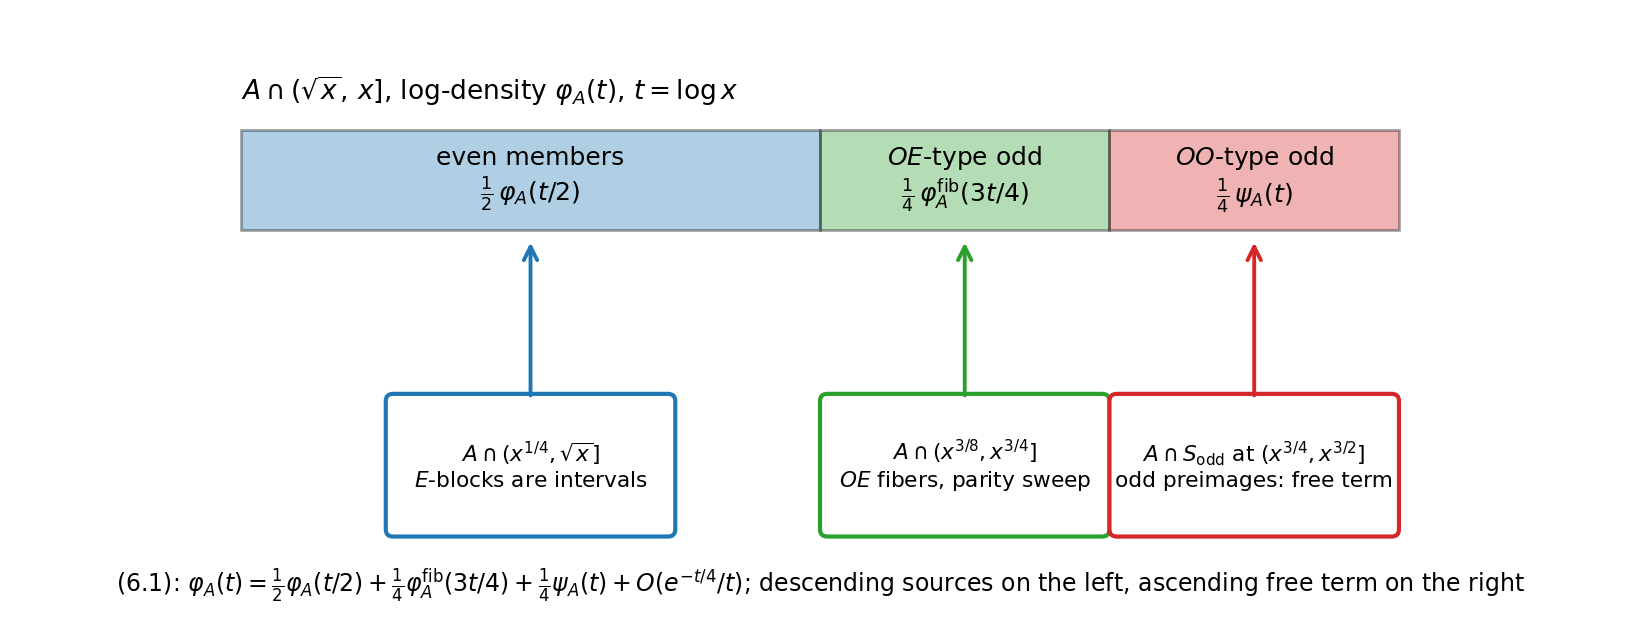
\includegraphics[width=1\linewidth,height=\textheight,keepaspectratio]{figures/paper_c_decomposition.png}
\caption{The first-letter decomposition of a two-way closed set on
\((\sqrt x,x]\): the even members come from scale \(x^{1/2}\) through
\(E\)-blocks, the \(OE\)-type odd members from scale \(x^{3/4}\) through
fibers, and the \(OO\)-type odd members are the odd preimages of the odd
images of \(A\) at scale \(x^{3/2}\) --- the free term.}
\end{figure}

\textbf{Definition 6.2 (\(S\)-fairness).} A two-way closed set \(A\) is
\emph{\(S\)-fair at scale \(t\)} if \(\psi_A(t)\le\varphi_A(3t/2)\),
i.e.~if \(A\) is not over-represented among the odd images of odd
integers at scale \(e^{3t/2}\) relative to its density among all
integers there; it is \emph{\(S\)-fair} if this holds for all
\(t\ge t_0\).

\textbf{Proposition 6.3 (exact statements).} (i) \(\psi_F\equiv 0\) iff
\(F=\emptyset\): if \(F\ne\emptyset\), its minimum is odd with odd
image, so \(\psi_F(t)>0\) on a shell containing \(\min F\). (ii) The
identity (6.1) holds for \(F\) with the stated error, and its right side
contains exactly one term, \(\tfrac14\psi_F(t)\), that is not determined
by \(F\) at smaller scales through the two productions.

\emph{Proof.} (i) If \(F=\emptyset\) then \(\psi_F\equiv 0\). If
\(F\ne\emptyset\), let \(n_F=\min F\). It is odd (an even failure has
the smaller failure \(\lfloor\sqrt{n_F}\rfloor\)), and its image is odd
(if \(J(n_F)\) were even, \(J^2(n_F)=\lfloor n_F^{3/4}\rfloor<n_F\)
would be a smaller failure). So \(n_F\) is an \(OO\)-type failure and
\(\psi_F(t)>0\) for \(t\) with \(e^{t/2}<n_F\le e^t\). (ii) is the
decomposition. \(\square\)

Lean: \texttt{\nolinkurl{minimal_failure_odd_odd}} and
\texttt{\nolinkurl{exists_minimal_failure}} (the least failure is odd
with odd image), and the three pieces as
\texttt{\nolinkurl{first_letter_trichotomy}} with
\texttt{\nolinkurl{first_letter_pieces_disjoint}}, in
\texttt{\nolinkurl{formal/Problems/Juggler/FateFirstLetter.lean}}; the
log-mass bookkeeping of (6.1) is not formalized.

\textbf{Remark 6.4 (the walk heuristic; not a theorem).} If \(F\) were
\(S\)-fair, if the fiber weights were ideal
(\(\varphi^{\rm fib}_F=\varphi_F\)), and if the error term of (6.1) were
zero, then (6.1) would give
\(\varphi_F(t)\le\tfrac12\varphi_F(t/2)+\tfrac14\varphi_F(3t/4)+\tfrac14\varphi_F(3t/2)\):
the harmonic inequality of a random walk on \(\log t\) with steps
\(\log\tfrac12,\log\tfrac34,\log\tfrac32\) of probabilities
\(\tfrac12,\tfrac14,\tfrac14\), whose drift \(-0.317\) is negative, so
that the boundary condition \(\varphi_F=0\) below \(\log N_0\) would
force \(\varphi_F\equiv 0\). None of the three conditions is available
with the constants proved here: the fiber weights are only known to lie
in \([\tfrac23,\tfrac43]\), so the coefficients of the inequality can
sum to \(\tfrac12+\tfrac13+\tfrac14=\tfrac{13}{12}>1\), and the boundary
error \(O(e^{-t/4}/t)\) is not zero at the scales just above the floor
where the walk exits. We therefore do not claim that \(S\)-fairness
implies the conjecture. What is exact is Proposition 6.3; what is proved
about the free term is Proposition 10.1, which identifies \(\psi_F(t)\)
with a quantity bounded by every hypothesis of Sections 8--9.

\subsection{6.3 Where Papers A and B
sit}\label{where-papers-a-and-b-sit}

Paper A {[}11{]} constrains the fate Lachesis from the inside: finance
and the walk charge bound the \emph{states} of a hypothetical cycle
(minimum \(>3.5\cdot 10^8\), period \(\ge 780239\)). Theorem 1
constrains the basin: if the cycle exists, its basin is a two-way closed
class with the cycle's states as seeds and log-count
\(\gg(\log x)^\lambda\) for every \(0<\lambda<\lambda^{**}\). In the
present argument the two estimates do not meet: finance bounds the seed,
contagion the growth from the seed, and no inequality bounds a basin
from above. Paper B {[}12{]} controls the descending branches of (6.1)
--- the fairness of the landing distributions of \(E\), \(OE\) and, with
its depth-4 and depth-5 theorems, of deeper contracting words --- on
dyadic blocks; Appendix C uses one statement of that type on sub-dyadic
intervals as an explicit hypothesis. Neither touches \(\psi_F\): the
ascending branch \(OO\) sends mass to \(x^{3/2}\), and its return is the
nested-floor parity at all depths.

\section{7. The almost-all
equivalence}\label{the-almost-all-equivalence}

\textbf{Corollary 7.1 (logarithmic form).} The following are equivalent:
(1) every \(n\ge 1\) reaches \(1\); (2) for some
\(\lambda<\lambda^{**}\),
\(\sum_{n\le x,\ n\notin R}1/n=o((\log x)^{\lambda})\); (3) for some
\(0<\lambda<\lambda^{**}\), the starts \(n\le x\) whose orbit never
enters \([1,N_0]\) have logarithmic count \(o((\log x)^{\lambda})\).

\emph{Proof.} (1)\(\Rightarrow\)(3): the set is empty.
(3)\(\Rightarrow\)(2): an orbit that enters \([1,N_0]\) reaches \(1\),
so \(F\) is contained in the set of (3). (2)\(\Rightarrow\)(1): \(F\) is
backward-closed; if it were nonempty, Theorem 5.3 would contradict (2).
\(\square\)

\textbf{Theorem 7.2 (a Tao-type bound with rate implies the
conjecture).} Suppose that for some \(e>1-\lambda^{**}\approx0.5074\)
and all sufficiently large \(y\), \[
\#\{n\ \text{odd},\ y<n\le 2y:\ n\notin R\}\ \le\ \frac{y}{(\log y)^{e}} .
\] Then \(R=\mathbb N\).

\emph{Proof.} By decreasing \(e\) if necessary, assume
\(1-\lambda^{**}<e<1\); the hypothesis is preserved for large \(y\).
Suppose \(F\ne\emptyset\). By Theorem 6.1 every \(n\in F\) lies in the
\(E\)-tree of an odd member of \(F\). For an odd \(n_0\in F\) the
level-\(j\) set \(S_j(n_0)\) of its \(E\)-tree has log-mass at most
\(\prod_{i<j}(1+n_0^{-2^i})/n_0\le 2/n_0\) (Lemma 3.1 gives
\(\sum_{n\in E(m)}1/n\le(m+1)/m^2\)), and only levels with
\(n_0^{2^j}\le x\), i.e.~\(j\le\log_2\log x\), meet \([1,x]\). Hence \[
\begin{aligned}
\sum_{\substack{n\in F\\n\le x}}\frac1n
&\le2(1+\log_2\log x)
 \sum_{\substack{n_0\in F\text{ odd}\\n_0\le x}}\frac1{n_0}\\
&\le2(1+\log_2\log x)
 \left(\sum_{k_0\le k\le\lfloor\log_2x\rfloor}(k\ln2)^{-e}+O(1)\right)\\
&\ll(\log x)^{1-e}\log\log x.
\end{aligned}
\] By Theorem 5.3 the left side is \(\ge K(\log x)^{\lambda}\) for every
\(\lambda<\lambda^{**}\) and all large \(x\). Choosing
\(\lambda\in(1-e,\lambda^{**})\) gives a contradiction. \(\square\)

\textbf{Theorem 7.3 (equivalence).} Every positive integer reaches \(1\)
if and only if there is \(e>1-\lambda^{**}\) such that
\(\#\{n\ \text{odd}\in(y,2y]:\ n\notin R\}\le y(\log y)^{-e}\) for all
large \(y\).

\emph{Proof.} If every integer reaches \(1\) the left side is \(0\).
Conversely Theorem 7.2. \(\square\)

The threshold \(1-\lambda^{**}\) is the complement of the contagion
exponent; with \(\lambda^{***}\) of Appendix C it becomes \(0.4608\).
Any improvement of the contagion exponent lowers the rate required of
the almost-all statement, and \(\lambda\to 1\) would make any positive
rate suffice --- but that improvement requires all descent certificates
and is circular here (Section 5.6).

\subsection{7.1 Comparison with the Collatz map: a structural
analogy}\label{comparison-with-the-collatz-map-a-structural-analogy}

The comparison with Tao's theorem {[}6{]} is a structural analogy, not a
transfer of methods, and it concerns two specific features.

\emph{Depth.} Juggler's multiplicative changes of \(\log n\) motivate a
walk on \(\log\log n\) and the depth \(O(\log\log y)\). This is the
depth used by the sufficient hypotheses here, not a proved stopping-time
bound for every orbit. For the accelerated Collatz map of Terras and
Everett, parity words of length \(k\) correspond to residue classes
modulo \(2^k\). Their counts in an interval of length \(y\) have an
additive \(O(1)\) boundary error; relative control by that fact alone
becomes ineffective once \(2^k\) is comparable to or larger than \(y\).
Saying that every depth of order \(\log y\) has singleton cylinders
would be too strong: the multiplicative constant in the depth matters.

\emph{Preimage counts.} The result of Krasikov--Lagarias {[}7{]} cited
in Section 1.3 has a different counting scale from Theorem 1. An
\(x^{0.84}\) lower bound is compatible with a bounded reciprocal sum,
and by itself cannot contradict a logarithmic error bound. This
comparison explains why the particular argument of Theorem 7.2 does not
transfer. It does not exclude other almost-all-to-all arguments for
Collatz.

Tao's theorem {[}6{]} has an arbitrarily slowly growing target and
logarithmic-density exceptional set. Our eventual-entry equivalence has
a fixed verified target and a specified dyadic rate; obtaining that rate
remains open. No part of Tao's renewal argument is claimed to have been
supplied for Juggler.

\section{8. From parity control to the almost-all
bound}\label{from-parity-control-to-the-almost-all-bound}

\subsection{8.1 Notation}\label{notation}

For a word \(w\in\{O,E\}^d\) and \(t\le d\) write \(o_t(w)\) for the
number of odd letters among the first \(t\) and \[
u_t(w)=o_t(w)\log_2 3-t
\] for the \emph{exponent walk}, so that the ideal image after \(t\)
letters is \(n^{2^{u_t}}\). For \(y>N_0\) put \[
L(y)=\log_2\frac{\log 2y}{\log N_0},\qquad d(y)=\lceil C\,L(y)\rceil ,
\] with a constant \(C\ge 5\) fixed below. A word \(w\) of length \(d\)
is \(L\)-\emph{bad} if \(u_t(w)>-L\) for every \(1\le t\le d\) (its walk
never descends to \(-L\)). \(\mathrm{word}_d(n)\) is the realized
itinerary of the first \(d\) steps of \(n\) (letter \(s\) is the parity
of \(J^{s-1}(n)\)); the \emph{cylinder} \([w]_y\) is the set of odd
\(n\in(y,2y]\) with \(\mathrm{word}_{|w|}(n)=w\). Odd starts have first
letter \(O\), so the fair share of an \(O\)-rooted cylinder of depth
\(d\) relative to the reference mass \(N=y/2\). The actual number of odd
starts in \((y,2y]\) is \(N+O(1)\); this bounded endpoint error is
absorbed in the asymptotic bounds below is \(2^{-(d-1)}N\).

\subsection{8.2 Envelope descent and the rarity of bad
words}\label{envelope-descent-and-the-rarity-of-bad-words}

\textbf{Lemma 8.1 (envelope descent).} Let \(n\in(y,2y]\) and
\(d\ge 1\). If \(\mathrm{word}_d(n)\) is not \(L(y)\)-bad, then
\(n\in R\).

\emph{Proof.} Some \(t\le d\) has \(u_t\le -L(y)\), i.e.
\(3^{o_t}/2^t\le\log N_0/\log 2y\le\log N_0/\log n\), i.e.
\(n^{3^{o_t}}\le N_0^{2^t}\) as integers. The power envelope
\(J^t(n)^{2^t}\le n^{3^{o_t}}\) (Paper A, Theorem 2.2;
\texttt{\nolinkurl{power_bound_word}}) gives \(J^t(n)\le N_0\), so
\(J^t(n)\in R\) and \(n\in R\) by backward closure. Lean:
\texttt{\nolinkurl{iterate_le_of_envelope}},
\texttt{\nolinkurl{mem_of_envelope_floor}},
\texttt{\nolinkurl{reachesOne_of_itinerary_envelope}}. \(\square\)

\textbf{Lemma 8.2 (Chernoff).} For \(C\ge 5\) put \[
p_C=\frac{1-1/C}{\log_2 3},\qquad
e(C)=\frac{C\,D(p_C\,\|\,\tfrac12)}{\ln 2},\qquad
D(p\|\tfrac12)=p\ln(2p)+(1-p)\ln(2(1-p)).
\] For \(L>0\) and \(d\ge CL\), the number of \(L\)-bad words of length
\(d\) is at most \(2^d\cdot 2^{-e(C)L}\). Moreover, for every
\(\varepsilon>0\) there is \(L_0\) such that for \(L\ge L_0\) and
\(d=\lceil CL\rceil\) the number of \(L\)-bad words of length \(d\)
beginning with \(O\) is at most
\(2^{d-1}\cdot 2^{-(e(C)-\varepsilon)L}\).

\emph{Proof.} An \(L\)-bad word has \(u_d>-L\), i.e.
\(o_d>(d-L)/\log_2 3\ge p_Cd\) (as \(L/d\le 1/C\)). For a fair coin,
\(\Pr[\mathrm{Bin}(d,\tfrac12)\ge pd]\le e^{-dD(p\|1/2)}\) for
\(p\ge\tfrac12\), and \(D(\cdot\|\tfrac12)\) is increasing on
\([\tfrac12,1]\); \(p_C\ge\tfrac12\) for \(C\ge 5\). Hence the count is
at most
\(2^de^{-dD(p_C\|1/2)}\le 2^de^{-CL\,D(p_C\|1/2)}=2^d2^{-e(C)L}\). For
the \(O\)-rooted count, the remaining \(d-1\) letters contain
\(o_d-1>(d-L)/\log_2 3-1=p'(d-1)\) odd letters with \(p'=p_C-O(1/L)\);
the same bound with \(d-1\) trials gives
\(2^{d-1}e^{-(d-1)D(p'\|1/2)}\), and
\((d-1)D(p'\|1/2)\ge(e(C)-\varepsilon)L\ln 2\) for \(L\) large.
\(\square\)

Lean: the first statement, in the exact form
\(\#\{w\ L\text{-bad},|w|=d\}\le 2^d\,2^{-e(C)L}\) for \(C\ge 5\),
\(d\ge CL\), \(d\ge 1\), is \texttt{\nolinkurl{LBad_count_le}} in
\texttt{\nolinkurl{formal/Problems/Juggler/FateChernoff.lean}}: the
Markov tilt \texttt{\nolinkurl{weight_markov}} on the constant weight
(\texttt{\nolinkurl{weightGen_one}}, \((1+x)^d\)), the value
\(\exp(d\,h(p))\) at \(x=p/(1-p)\) (\texttt{\nolinkurl{tilt_value}},
\texttt{\nolinkurl{count_oddCount_ge_le_exp}}), Gibbs' inequality
\(D(p\|\tfrac12)\ge 0\) (\texttt{\nolinkurl{klHalf_nonneg}}), and
\(p_C\in[\tfrac12,1)\) from \(\log_2 3\le 8/5\)
(\texttt{\nolinkurl{half_le_pC}}, \texttt{\nolinkurl{pC_lt_one}}). The
\(O\)-rooted statement with \(\varepsilon\) stays a human proof.

Numerically \(e(18)\approx0.480\), \(e(19)\approx0.527\),
\(e(20)\approx0.574\), \(e(21)=0.621\), \(e(25)=0.812\),
\(e(30)=1.054\); \(e(C)\) grows linearly in \(C\) with slope
\(D(1/\log_2 3\,\|\,\tfrac12)/\ln 2=0.050\).

\subsection{8.3 The cylinder hypothesis and the
bound}\label{the-cylinder-hypothesis-and-the-bound}

\textbf{Hypothesis \(\mathrm H(C,A)\) (log-log-depth cylinder bound).}
For all sufficiently large \(y\), with \(d=d(y)\), every word
\(w\in\{O,E\}^d\) that begins with \(O\) and is \(L(y)\)-bad satisfies
\[
\#[w]_y\ \le\ 2^{-(d-1)}\cdot\frac y2+\frac{y}{(\log y)^{A}} .
\]

Only an upper bound is asked, only at one depth per scale, and only for
the \(L(y)\)-bad words. Since \(2^{-(d-1)}y/2\asymp y(\log y)^{-C}\),
\(\mathrm H(C,A)\) with \(A>C\) says that no \(O\)-rooted cylinder of
depth \(d(y)\) whose envelope has not crossed the floor exceeds its fair
share by more than a relative \(O((\log y)^{C-A})\). The restriction is
essential: the older all-word version is false because already absorbed
starts can share a long terminating tail and overpopulate a cylinder
without contributing any live mass; see the
\href{https://github.com/sneakyweasel/btlab/blob/main/docs/problems/juggler_absorbed_cylinder.md}{absorbed-cylinder
obstruction}. This obstruction does not refute \(\mathrm H(C,A)\) as
stated here.

\textbf{Theorem 8.3 (Tao-type bound from the cylinder hypothesis).}
Assume \(\mathrm H(C,A)\) with \(C\ge 5\) and \(A>C+e(C)\). Then for
every \(\varepsilon>0\) and all sufficiently large \(y\), \[
\begin{aligned}
\#\{n\text{ odd in }(y,2y]:n\notin R\}
&\le\#\{n\text{ odd in }(y,2y]:J^t(n)>N_0\ \forall t\le d(y)\}\\
&\le\frac y2\left(\frac{\log(2y)}{\log N_0}\right)^{-(e(C)-\varepsilon)}.
\end{aligned}
\] In words: all but \(O(y(\log y)^{-e(C)+\varepsilon})\) odd starts in
\((y,2y]\) enter \([1,N_0]\) within \(d(y)=O(\log\log y)\) steps.

\emph{Proof.} A failure never enters the verified floor, giving the
first inequality. A live start has a bad word by Lemma 8.1. Apply Lemma
8.2 with \(\varepsilon/2\) in place of \(\varepsilon\). Every odd start
has an \(O\)-rooted word; by Lemma 8.2 the \(O\)-rooted bad words number
at most \(2^{d-1}2^{-(e(C)-\varepsilon/2)L(y)}\), and by
\(\mathrm H(C,A)\) each carries at most \(2^{-(d-1)}y/2+y(\log y)^{-A}\)
odd starts. Hence the count is at most \[
\frac y2\,2^{-(e(C)-\varepsilon/2)L(y)}+2^{d-1}\,\frac{y}{(\log y)^A}
\ \le\ \frac y2\Bigl(\frac{\log 2y}{\log N_0}\Bigr)^{-(e(C)-\varepsilon/2)}
+\Bigl(\frac{\log 2y}{\log N_0}\Bigr)^{C}\frac{y}{(\log y)^{A}},
\] using \(2^{d-1}\le 2^{CL}\). The second term is
\(O(y(\log y)^{C-A})=o(y(\log y)^{-e(C)})\) because \(A>C+e(C)\). For
large \(y\), both terms fit inside the displayed bound with exponent
\(e(C)-\varepsilon\), using the remaining \(\varepsilon/2\) slack.
\(\square\)

Lean: the exact skeleton, in
\texttt{\nolinkurl{formal/Problems/Juggler/FateChernoff.lean}}.
\texttt{\nolinkurl{oddFailures_subset_bad_cylinders}} is Lemma 8.1 in
covering form: with every start up to \(N_0\) reaching \(1\), an odd
\(n\in(y,2y]\) that does not reach \(1\) lies in the cylinder of a word
whose every prefix fails the integer envelope comparison
\(N_0^{2^t}<(2y)^{3^{o_t}}\) (\texttt{\nolinkurl{EnvelopeBad}});
\texttt{\nolinkurl{LBad_of_envelopeBad}} identifies those words as
\(L(y)\)-bad with \(L(y)=\log_2(\log 2y/\log N_0)\);
\texttt{\nolinkurl{oddFailures_card_le}} is the union bound, and
\texttt{\nolinkurl{oddFailures_card_le_chernoff}} composes it with Lemma
8.2: if every \(L(y)\)-bad cylinder of depth \(d\ge CL(y)\) holds at
most \(M\) starts, the odd failures in \((y,2y]\) number at most
\(2^d\,2^{-e(C)L(y)}M\).
\texttt{\nolinkurl{oddFailures_card_le_explicit}} substitutes
\(d=\lceil CL(y)\rceil\) and the bound of \(\mathrm H(C,A)\) at the
scale \(y\), for \(O\)-rooted words only
(\texttt{\nolinkurl{cylinder_even_root_empty}}): with
\(\Lambda=\log 2y/\log N_0\), the odd failures in \((y,2y]\) number at
most \(y\,\Lambda^{-e(C)}+2\Lambda^{C}y(\log y)^{-A}\), at every
\(y\ge 2\) and without \(\varepsilon\). The displayed form follows by
absorbing the factor \(2\) into \(\Lambda^{\varepsilon}\) and the second
term into the first for \(A>C+e(C)\); that absorption is not formalized.
Corollary 8.4 uses only the exponent.

\textbf{Corollary 8.4 (the conjecture from a cylinder bound).} If
\(\mathrm H(C,A)\) holds for some \(C\ge 19\) and \(A>C+e(C)\), then
every positive integer reaches \(1\). Under the conditional exponent
\(\lambda^{***}\) of Appendix C the same conclusion holds for
\(C\ge 18\).

\emph{Proof.} Theorem 8.3 gives the hypothesis of Theorem 7.2 with
\(e=e(C)-\varepsilon\ge e(19)-\varepsilon>1-\lambda^{**}\); with
\(\lambda^{***}\) the threshold is \(0.4608<e(18)\approx0.480\). The
pairing-only intermediate still needed \(C\ge 20\)
(\(e(20)=0.574>0.5520\)). \(\square\)

\subsection{8.4 Constants}\label{constants}

The least integer depth constant in this sufficient criterion is
\(C=19\) (\(e(19)\approx0.527>1-\lambda^{**}\)). With the certified
floor \(N_0=3.5\cdot 10^8\), the table below keeps \(C=20\) as a
conservative a-fortiori display:

\begingroup\small

\begin{longtable}[]{@{}
  >{\raggedright\arraybackslash}p{(\linewidth - 10\tabcolsep) * \real{0.1667}}
  >{\raggedright\arraybackslash}p{(\linewidth - 10\tabcolsep) * \real{0.1667}}
  >{\raggedright\arraybackslash}p{(\linewidth - 10\tabcolsep) * \real{0.1667}}
  >{\raggedright\arraybackslash}p{(\linewidth - 10\tabcolsep) * \real{0.1667}}
  >{\raggedright\arraybackslash}p{(\linewidth - 10\tabcolsep) * \real{0.1667}}
  >{\raggedright\arraybackslash}p{(\linewidth - 10\tabcolsep) * \real{0.1667}}@{}}
\toprule\noalign{}
\begin{minipage}[b]{\linewidth}\raggedright
\(y\)
\end{minipage} & \begin{minipage}[b]{\linewidth}\raggedright
\(L(y)\)
\end{minipage} & \begin{minipage}[b]{\linewidth}\raggedright
\(d(y)\)
\end{minipage} & \begin{minipage}[b]{\linewidth}\raggedright
exact fair-coin bad probability
\end{minipage} & \begin{minipage}[b]{\linewidth}\raggedright
\((\log y)^{-0.6}\)
\end{minipage} & \begin{minipage}[b]{\linewidth}\raggedright
least depth for rate \(0.6\)
\end{minipage} \\
\midrule\noalign{}
\endhead
\bottomrule\noalign{}
\endfoot
\bottomrule\noalign{}
\endlastfoot
\(10^{20}\) & \(1.25\) & \(25\) & \(0.065\) & \(0.100\) & \(19\) \\
\(10^{100}\) & \(3.55\) & \(72\) & \(0.017\) & \(0.038\) & \(56\) \\
\(10^{1000}\) & \(6.87\) & \(138\) & \(0.0038\) & \(0.0096\) &
\(117\) \\*
\end{longtable}

\endgroup

The bad probability is the fair-coin probability that a walk of length
\(d(y)\) never reaches \(-L(y)\), by dynamic programming over the walk
(unconditioned first letter; conditioning on \(u_1=\log_2 3-1\) roughly
doubles the finite-depth values and leaves the exponent unchanged); the
last column is the least depth at which it drops below
\((\log y)^{-0.6}\) --- about \(17\,L(y)\). With the Lean floor
\(N_0=260\) the depths grow by about \(38\) letters. For comparison,
Paper B controls depth \(4\) (all words) and two words of depth \(5\),
with relative error \(y^{-1/96}\) on dyadic blocks; the hypothesis asks
for the bad cylinders at depth \(d(y)\to\infty\) with relative error
\(o(1)\) --- weaker in rate than a power saving, unbounded in depth.

\section{9. Weaker forms of the
hypothesis}\label{weaker-forms-of-the-hypothesis}

Theorem 8.3 asks for a fair-share upper bound on every envelope-bad
cylinder at one depth. Lower bounds and control of cylinders after their
envelope has crossed the floor are not needed. This section gives the
sufficient conditions, including a single moment bound, and records what
that form does not need.

\subsection{9.1 One-sided odd-share
control}\label{one-sided-odd-share-control}

\textbf{Hypothesis \(\mathrm H_q(C,A)\).} For all sufficiently large
\(y\), every \(1\le t<d(y)\) and every \(L(y)\)-bad word
\(w\in\{O,E\}^t\), \[
\#\{n\in[w]_y:\ \mathrm{word}_{t+1}(n)=wO\}\ \le\ q\,\#[w]_y+\frac{y}{(\log y)^{A}} .
\] (The depth-\(0\) cylinder is all odd starts, whose next letter is
\(O\) with share \(1\); the hypothesis starts at depth \(1\). As in
Section 8.3, no condition is imposed after an envelope crossing.)

\textbf{Theorem 9.1 (one-sided form).} Let \(0<q<\log 2/\log 3=0.6309\),
\(\mu=1-q\log_2 3>0\), \(C>1/\mu\), and
\(e_q(C)=2(C\mu-1)^2/(C(\log_2 3)^2\ln 2)\). Under \(\mathrm H_q(C,A)\)
with \(A>C+e_q(C)\), for every \(\varepsilon>0\) and all large \(y\), \[
\#\{n\ \text{odd}\in(y,2y]:\ n\notin R\}\ \le\ \frac y2\Bigl(\frac{\log 2y}{\log N_0}\Bigr)^{-(e_q(C)-\varepsilon)} .
\] Hence \(e_q(C)>1-\lambda^{**}\) implies the conjecture; the least
\(C\) is \(19\) at \(q=\tfrac12\), \(41\) at \(0.55\), \(223\) at
\(0.60\), \(1586\) at \(0.62\) (with \(\lambda^{***}\): \(18\), \(39\),
\(206\), \(1451\)).

\emph{Proof.} Let \(n\) be uniform on the \(N_y=y/2+O(1)\) odd integers
of \((y,2y]\). Bounded endpoint factors are absorbed using
\(\varepsilon\)-slack. Follow its actual word until the first prefix
that is not \(L(y)\)-bad, and after that crossing append synthetic
letters \(E\). Let \(\widehat{\mathcal F}_t\) be the filtration of these
stopped words, \(\widehat X_t\) the indicator that the synthetic next
letter is \(O\), and \(\widehat u_t=(\log_2 3-1)+
\sum_{1\le s<t}(\widehat X_s\log_2 3-1)\). On a bad atom the stopped
word is the actual word, so \(\mathrm H_q\) applies; on a crossed atom
\(\widehat X_t=0\). Thus, with
\(\eta_t=(\mathbb P(\widehat X_t=1\mid\widehat{\mathcal F}_t)-q)^+\),
each bad atom \([w]\) has \(\eta_t\le y(\log y)^{-A}/\#[w]\), while
every crossed atom has \(\eta_t=0\). There are at most \(2^t\) atoms, so
\(\mathbb E[\eta_t]\ll 2^t(\log y)^{-A}\) and
\(\mathbb E[\sum_{1\le t<d}\eta_t]\ll (\log 2y/\log N_0)^{C}(\log y)^{-A}\).
Since
\(\mathbb E[\widehat u_{t+1}-\widehat u_t\mid\widehat{\mathcal F}_t]
\le-\mu+\eta_t\log_2 3\), the process \(M_t=\widehat u_t-\widehat u_1-
\sum_{1\le s<t}\mathbb E[\widehat u_{s+1}-\widehat u_s
\mid\widehat{\mathcal F}_s]\) is a martingale with increments in an
interval of length \(\log_2 3\), and
\(\widehat u_d\le \widehat u_1+M_d-(d-1)\mu+
\log_2 3\sum_{s<d}\eta_s\). Fix \(\kappa\in(0,1)\). If \(n\notin R\),
the contrapositive of Lemma 8.1 gives \(u_t>-L\) for every \(t\le d\).
Thus no crossing occurred, \(\widehat u_d=u_d>-L\), and hence either
\(\log_2 3\sum_s\eta_s>\kappa(d-1)\mu\), an event of probability
\(O((\log y)^{C-A})\) by Markov's inequality, which is
\(o((\log y)^{-e_q(C)+\varepsilon})\) under the stated condition, or
\(M_d>a:=(1-\kappa)(d-1)\mu-L-\widehat u_1
\ge L((1-\kappa)C\mu-1)-\log_2 3\). By the Azuma--Hoeffding inequality,
\(\mathbb P(M_d>a)\le\exp(-2a^2/((d-1)(\log_2 3)^2))\le 2^{-L(e_q^{(\kappa)}(C)-o(1))}\)
with
\(e_q^{(\kappa)}(C)=2((1-\kappa)C\mu-1)^2/(C(\log_2 3)^2\ln 2)\to e_q(C)\)
as \(\kappa\to 0\). \(\square\)

So no lower bound on odd shares and no vanishing error are needed: if no
\(L(y)\)-bad cylinder of depth below \(41\log_2(\log 2y/\log N_0)\)
sends more than \(55\%\) of its members to an odd state, every positive
integer reaches \(1\).

\subsection{9.2 The pressure form}\label{the-pressure-form}

Let \(N=y/2\), let \(\tau(n)=\min\{t\ge1:J^t(n)\le N_0\}\), with
\(\min\emptyset=\infty\), be the entrance time into the floor, call
\(n\) \emph{live at depth \(t\)} if \(\tau(n)>t\), and write \(o_t(n)\)
for the number of odd letters among \(n,J(n),\dots,J^{t-1}(n)\). By
Lemma 8.1, \(\tau(n)>t\) implies \(u_t(n)>-L(y)\). The stopping is
essential: \(J(1)=1\) is odd, so an orbit that has reached \(1\) has an
all-\(O\) tail and the unstopped odd count of every start in \(R\) grows
linearly. For \(\theta>0\) put \(a_\theta=\tfrac12(1+e^{\theta})\).

\textbf{Hypothesis \(\mathrm P_\theta(C)\) (live pressure).} For all
sufficiently large \(y\), with \(d=d(y)\), \[
\frac1N\sum_{\substack{n\ \mathrm{odd}\in(y,2y]\\ \tau(n)>d}}e^{\theta\,o_d(n)}
\ \le\ a_\theta^{\,d}\,e^{o(d)} .
\]

\textbf{Theorem 9.2 (pressure form).} Assume \(\mathrm P_\theta(C)\)
with \(C\ge 5\) and \(\theta=\theta_C=\log\bigl(p_C/(1-p_C)\bigr)\).
Then for every \(\varepsilon>0\) and all large \(y\), \[
\#\{n\ \mathrm{odd}\in(y,2y]:\ \tau(n)>d(y)\}
\ \le\ \frac y2\Bigl(\frac{\log 2y}{\log N_0}\Bigr)^{-(e(C)-\varepsilon)},
\] the bound of Theorem 8.3. Hence \(\mathrm P_{\theta_C}(C)\) with
\(C\ge 19\) implies the conjecture using Theorem 1, and with \(C\ge 18\)
under the conditional exponent of Appendix C.

\emph{Proof.} If \(\tau(n)>d\) then \(u_d>-L\), i.e.~\(o_d\ge p_Cd\).
Hence \[
\#\{\tau>d\}\le\#\{\tau>d,\ o_d\ge p_Cd\}
\le e^{-\theta p_Cd}\sum_{\tau(n)>d}e^{\theta o_d(n)}
\le N\,e^{-\theta p_Cd}a_\theta^{\,d}e^{o(d)} .
\] At \(\theta=\theta_C\),
\(\theta p_C-\log a_\theta=D(p_C\|\tfrac12)\), so the count is
\(\le N\exp(-dD(p_C\|\tfrac12)(1-o(1)))\le N2^{-(e(C)-\varepsilon)L}\).
\(\square\)

Lean: exact form, in
\texttt{\nolinkurl{formal/Problems/Juggler/FatePressure.lean}}, on the
live weight of \texttt{\nolinkurl{LiveCountWeight}} (starts in
\(\{1,\dots,N\}\) that stay above \(N_0\) for \(d\) steps).
\texttt{\nolinkurl{livePressure}} is
\(\sum_{n\ \mathrm{live}}x^{o_d(n)}\) as the generating function of the
live weight; \texttt{\nolinkurl{live_count_le_pressure}} is the Markov
step \(\#\{\text{live},\,o_d\ge k\}\le\text{pressure}/x^k\);
\texttt{\nolinkurl{live_oddCount_ge}} is Lemma 8.1 on live starts
(\(o_d\ge p_Cd\) for \(d\ge CL(N)\)); and
\texttt{\nolinkurl{live_count_le_of_pressure}} says: if the pressure at
the tilt \(x=p_C/(1-p_C)\) is at most \(Na_\theta^dE\), the live starts
number at most \(N\exp(-dD(p_C\|\tfrac12))E\), by the identity
\(a_\theta^d/x^{p_Cd}=e^{-dD(p_C\|1/2)}\)
(\texttt{\nolinkurl{tilt_value}}). The substitution \(E=e^{o(d)}\) and
\(d=\lceil CL\rceil\) that gives the displayed bound is not formalized.

For \(1\le t<d\) let \(\mu_{\theta,t}\) be the probability measure on
the starts live at depth \(t\) with density proportional to
\(e^{\theta o_t(n)}\), and let
\(s_\theta(t)=\mu_{\theta,t}(J^t(n)\ \text{odd})\) be the \emph{tilted
odd share}: the probability that the next letter is \(O\) when odd-heavy
live prefixes are up-weighted exponentially. If the live set is empty,
define \(s_\theta(t)=0\); subsequent live moments are then zero.

\textbf{Hypothesis \(\mathrm M_{\theta,q}(C)\) (no momentum).} For all
large \(y\), \(\sum_{t=1}^{d(y)-1}\bigl(s_\theta(t)-q\bigr)^+=o(d(y))\).

\textbf{Proposition 9.3.} \(\mathrm M_{\theta,1/2}(C)\) implies
\(\mathrm P_\theta(C)\). More generally, for \(0<q<1\) and a fixed
\(\theta>0\), \(\mathrm M_{\theta,q}(C)\) gives \[
\#\{\tau>d\}\le
N\exp\{-d[\theta p_C-\log(1-q+qe^\theta)-o(1)]\}.
\] If \(0<q<p_C<1\) and the hypothesis is assumed at the optimizing tilt
\(\theta=\theta_{C,q}:=\log\frac{p_C(1-q)}{q(1-p_C)}\), this becomes
\(N\exp(-dD(p_C\|q)(1-o(1)))\), with exponent
\(e_q^{\rm Ch}(C)=C\,D(p_C\|q)/\ln 2\), at least the Azuma exponent of
Theorem 9.1. Its least \(C\) at \(q=0.5,0.55,0.60,0.62\) is
\(19,41,214,1496\) (with \(\lambda^{***}\): \(18,38,198,1369\)).

\emph{Proof.} Dropping the condition \(\tau>t+1\) in favour of
\(\tau>t\) only enlarges the sum, so \[
\sum_{\tau>t+1}e^{\theta o_{t+1}}\le\sum_{\tau>t}e^{\theta o_{t+1}}
=\Bigl(\sum_{\tau>t}e^{\theta o_t}\Bigr)\bigl(1+(e^{\theta}-1)s_\theta(t)\bigr).
\] With \(a_{\theta,q}=1+(e^\theta-1)q\) and
\(c_\theta=(e^\theta-1)/a_{\theta,q}\),
\(1+(e^\theta-1)s\le a_{\theta,q}\exp\bigl(c_\theta(s-q)^+\bigr)\).
Telescoping from \(t=1\) gives
\(\sum_{\tau>d}e^{\theta o_d}\le Ne^{\theta}a_{\theta,q}^{\,d-1}\exp\bigl(c_\theta\sum_{t<d}(s_\theta(t)-q)^+\bigr)\),
which is \(\mathrm P_\theta\) at \(q=\tfrac12\). For general \(q\), the
exponential Markov step gives \(\theta p_C-\log a_{\theta,q}\) at the
same fixed \(\theta\). Assuming \(\mathrm M_{\theta,q}\) at
\(\theta=\log\frac{p_C(1-q)}{q(1-p_C)}\) gives \(D(p_C\|q)\).
\(\square\)

Lean: \texttt{\nolinkurl{weightGen_succ_le_share}} (the one-depth step),
\texttt{\nolinkurl{one_add_le_exp_excess}},
\texttt{\nolinkurl{weightGen_le_pressure}} (the telescoped bound) and
\texttt{\nolinkurl{count_le_pressure}} (the exponential Markov step), in
\texttt{\nolinkurl{formal/Problems/Juggler/TiltedShare.lean}}, on the
word-weight framework of \texttt{\nolinkurl{RateFreeDensity}};
\texttt{\nolinkurl{tilt_exponent_eq_kl}} is the identity at the
re-centring tilt.

\subsection{9.3 Scope of the moment
criterion}\label{scope-of-the-moment-criterion}

\textbf{(a) Any \(o(\log\log y)\) initial depths are free.} A letter
contributes a factor at most \(e^\theta\) to the moment, so bias ---
however extreme --- at any set of depths of size \(o(d(y))\) is absorbed
by the \(e^{o(d)}\). In particular the depth-five split (Paper B's
Conjecture 7.3) and every split to any fixed depth, or to depth
\(s_0(y)\) for any \(s_0=o(\log\log y)\), is irrelevant to the
reduction.

\textbf{(b) A tower comparison in a model population.} Suppose a model
cylinder \(O^t\) has size \(N\beta^{t-1}\). Its moment relative to the
fair \emph{reference} total \(Ne^\theta a_\theta^{t-1}\) is
\((\beta e^\theta/a_\theta)^{t-1}\). This ratio decays precisely when
\(\beta<(1+e^{-\theta})/2\), about \(0.836\) at
\(\theta_{19}\approx0.396\). Its count alone exceeds the reference
survival exponent only when \(\beta>2^{-e(C)/C}\), about \(0.981\) at
\(C=19\).

These are algebraic comparisons to a reference mass. They do not bound
\(s_\theta(t)\) in an actual stopped population, whose total live mass
may be much smaller. A model tower below \(0.836\) is therefore not, by
itself, a proof of the no-momentum hypothesis.

\textbf{(c) One-sidedness and aggregation.} \(\mathrm M_{\theta,q}\)
bounds the accumulated positive excess of a weighted average over
depths. Under-populated odd continuations can offset excess within the
same depth; over-populated cylinders contribute in proportion to their
tilted weight. In Walsh terms,
\(e^{\theta X_s}=a_\theta+b_\theta(-1)^{J^s(n)}\) with
\(b_\theta/a_\theta=-\tanh(\theta/2)\), so the unstopped moment is \[
\frac1N\sum_ne^{\theta o_d(n)}=a_\theta^{\,d}\Bigl(1+\sum_{\emptyset\ne T}(-\tanh\tfrac\theta2)^{|T|}\frac{W_T}{N}\Bigr),
\qquad W_T=\sum_n\prod_{s\in T}(-1)^{J^s(n)} :
\] Walsh sums of high order are exponentially down-weighted
(\(\tanh(0.198)=0.196\) per letter), whereas \(\mathrm H(C,A)\) asks for
a separate supremum bound on each \(L(y)\)-bad cylinder at the target
depth.

\textbf{(d) Other sufficient statistics.} The proof of Theorem 9.1 also
works if the odd-share bound fails only on bad atoms of total
probability \(O((\log y)^{-B})\) at each depth, with \(B>e_q(C)\): the
expected accumulated excess is \(O(d(\log y)^{-B})\), and Markov's
inequality absorbs it.

For comparison, let \(D(w)=\#[wO]-\tfrac12\#[w]\),
\(\mathcal C_t=\sum_{|w|=t}\#[w]^2\), and let \(W_T\) be the Walsh sums
on the same full set of odd starts. Parseval gives the exact identities
\[
\sum_w D(w)^2=2^{-t-2}\sum_{S\subseteq\{0,\ldots,t-1\}}
 |W_{S\cup\{t\}}|^2
 =\tfrac12\mathcal C_{t+1}-\tfrac14\mathcal C_t.
\] An additional quantitative bound on these sums can supply an
exceptional-atom estimate. No rate-independent equivalence with the
restricted bad-cylinder hypothesis is asserted. Full-population fair
collision bounds also face the absorbed-cylinder obstruction of Section
8.3.

\textbf{(e) Bounded-depth statistics and the walk model.} Fix \(k\). The
probability measure on parity words that is fair to depth \(k\) and
all-\(O\) afterwards satisfies every cylinder-count statement of depth
\(\le k\) exactly, and under it a positive proportion of model walks
never crosses the barrier. An argument for the Tao-type bound that used
only depth-\(\le k\) cylinder statistics of the Juggler map and the walk
logic would prove the same bound for that measure. Thus finite-depth
statistics plus the envelope walk alone are insufficient. This model
example does not rule out a proof using additional arithmetic properties
of the Juggler map.

\subsection{9.4 Where the difficulty
lies}\label{where-the-difficulty-lies}

\(\mathrm P_\theta(C)\) says that the exponentially tilted distribution
of live parity words of length \(d\asymp\log_2\log y\) has the fair
pressure \(\log a_\theta\): odd-heavy live words --- those with about
\(e^\theta/(1+e^\theta)\approx 60\%\) odd letters, the words the tilt
selects --- are not over-populated at an exponential rate in \(d\).
Typical such words contain odd runs of length \(\ge 4\), so the nested
towers of height \(\ge 4\) that stop Paper B at depth five sit inside
almost every relevant cylinder; but no individual cylinder is required
to split fairly, only the tilted average over the \(\approx 2^{0.97d}\)
typical cylinders at each depth. This is a statement about averaging
over cylinders at unbounded depth --- a mean over characters, not a
supremum --- of a kind for which analytic number theory sometimes has
tools where pointwise bounds fail. We record the question and do not
pursue an analytic approach here.

\section{10. The free term and limits of the
reductions}\label{the-free-term-and-limits-of-the-reductions}

\subsection{10.1 The free term is the infinite-depth live
mass}\label{the-free-term-is-the-infinite-depth-live-mass}

Recall the free term \(\psi_F\) of (6.1). For odd \(n\),
\(n\in F\iff\lfloor n^{3/2}\rfloor\in F\) (Theorem 6.1), and
\(n\in F\iff\tau(n)=\infty\) since \([1,N_0]\subseteq R\). Let
\(\mathbb P^{\log}_x\) be the \(1/n\)-weighted measure on the odd
\(n\in(\sqrt x,x]\).

\textbf{Proposition 10.1 (normalized live limit).} Put \[
q_{OO}(t)=\frac8t
 \sum_{\substack{\sqrt x<n\le x\\ \mathrm{word}_2(n)=OO}}\frac1n,
\qquad x=e^t.
\] Whenever the conditioning set is nonempty, \[
\psi_F(t)=q_{OO}(t)\lim_{d\to\infty}
 \mathbb P_x^{\log}(\tau(n)>d\mid\mathrm{word}_2(n)=OO).
\tag{10.1}
\] The limit is decreasing. For large \(t\),
\(q_{OO}(t)=1+O(e^{-\delta t})\) for some \(\delta>0\). If a hypothesis
in Sections 8--9 gives a live-start bound with rate \(r>0\), then, for
every \(0<\varepsilon<r\), \[
\psi_F(t)\ll_\varepsilon
 \left(\frac{t}{2\log N_0}\right)^{-(r-\varepsilon)}.
\tag{10.2}
\] For the one-sided and no-momentum forms, the same proofs bound live
starts as well as failures. The rate is the case-dependent rate in
Theorem 4.

\emph{Proof.} At fixed \(x\) the conditioning set is finite, and
\(F=\{n:\tau(n)=\infty\}\). Continuity for decreasing events gives
(10.1), including its normalization factor. The depth-two parity
estimate for odd starts gives \(OO\)-count \(y/4+O(y^{1-\delta'})\) on
dyadic blocks. Partial summation, or the same exponential-sum bound on
initial subintervals, gives the asserted reciprocal-mass asymptotic for
\(q_{OO}\).

Cover \((\sqrt x,x]\) by downward dyadic blocks, allowing one partial
block at the lower end. On \((y,2y]\) the reciprocal mass of live starts
is at most their count divided by \(y\), hence
\(O((\log y/\log N_0)^{-(r-\varepsilon)})\). There are \(O(t)\) blocks
and \(\log y\ge t/2-O(1)\). Multiplication by \(8/t\), the definition of
\(\psi_F\), proves (10.2). No equality between an unweighted block ratio
and its reciprocal-weighted ratio is used. \(\square\)

This connects the free term with live counts. The decreasing limit does
not provide a rate of convergence in depth; the finite-depth estimates
remain additional sufficient hypotheses.

\subsection{10.2 What the upper recursion
proves}\label{what-the-upper-recursion-proves}

Equations (6.1) and the fiber upper bound give, for large \(t\), \[
\varphi_F(t)\le\tfrac12\varphi_F(t/2)
 +\tfrac13\varphi_F(3t/4)+\tfrac14\psi_F(t)+O(e^{-\delta t}).
\tag{10.3}
\] The coefficient is \(1/3\) with the proved upper share; the ideal
fiber model would replace it by \(1/4\). If \(c\) denotes either
coefficient, the homogeneous exponent \(e_c>0\) is the root of
\(\tfrac12 2^{e_c}+c(4/3)^{e_c}=1\). Numerically it is \(0.3391\) for
\(c=1/3\), and \(1-\lambda_{\rm ideal}=0.5073\) for \(c=1/4\). These
values describe the upper comparison, not a proved exact decay rate of a
nonempty failure set.

\textbf{Corollary 10.2 (upper comparison).} If \(\psi_F(t)=O(t^{-r})\)
for some \(r>0\), then \(\varphi_F(t)=O(t^{-a})\) for every
\(0<a<\min(r,e_c)\), using \(c=1/3\) in (10.3). The ideal model has the
analogous assertion with \(c=1/4\). The upper inequality alone does not
imply \(F=\emptyset\).

\emph{Proof.} For such \(a\), \(h=\tfrac12 2^a+c(4/3)^a<1\). Choose a
large initial scale \(T\) and then \(K\) so that
\(\varphi_F(t)\le Kt^{-a}\) on \([T/2,T]\), and so that the forcing in
(10.3) is bounded by \((1-h)Kt^{-a}\) for \(t\ge T\). Induction on
intervals \([T,(4/3)^jT]\) proves the bound. At the endpoint \(a=e_c\)
there is no slack; in particular an endpoint estimate cannot be inferred
by the same argument. A positive multiple of \(t^{-e_c}\) satisfies the
homogeneous comparison on a tail, so that comparison alone does not
force the function to vanish. The lower contagion estimates and this
upper comparison do not establish a matching asymptotic. \(\square\)

\subsection{10.3 The depth-uniformity
budget}\label{the-depth-uniformity-budget}

Section 9.3(e) limits what fixed-depth statistics plus the envelope walk
alone can prove. The form of Theorem 8.3 says how uniform that
information must be \emph{along the cylinder-count route}.

\textbf{Proposition 10.3 (depth-uniformity budget).} Suppose the
available cylinder discrepancy bound is \[
\left|\#[w]_y-2^{-(d-1)}y/2\right|
 \le K2^{\kappa d}y^{1-\delta_0 2^{-cd}},
\] for the relevant bad words, with constants \(K,\delta_0,c>0\),
\(\kappa\ge0\), and a scale threshold independent of \(d\). At
\(d=C\log_2\log y+O(1)\), the resulting error majorant after summing
over at most \(2^d\) words is \(o(y(\log y)^{-r})\) for every fixed
\(r>0\) if and only if \(cC<1\).

\emph{Proof.} Divide the error majorant by \(y(\log y)^{-r}\) and take
logarithms. The result is \[
O(1)+((\kappa+1)C+r)\log\log y
 -\Theta((\log y)^{1-cC}).
\] It tends to \(-\infty\) exactly when \(cC<1\). If \(cC\ge1\), this
majorant is insufficient; the actual error may still be much smaller.
Without uniform control of the prefactor and the scale threshold, a
bound at every fixed depth would not justify any conclusion at growing
depth. \(\square\)

At \(C=19\) this requires the saving exponent to lose less than a factor
\(2^{1/19}=1.037\) per depth; at \(C=41\), \(2^{1/41}=1.017\). Weyl
differencing loses a factor \(2^{c}\) with \(c\ge1\) per differencing
(Paper B's chain \(\tfrac1{24}\to\tfrac1{96}\) from depth three to four
is \(c=2\)), and with such a loss the cylinder-count route reaches depth
\(\approx\log_2\log y\) --- one unit of \(L(y)\), enough for the
all-\(E\) word to reach the floor, not for the Chernoff tail, which
needs \(C\ge 5\) units. The proposition is narrow by design: it concerns
methods whose only available error estimate deteriorates exponentially
in the depth and are used through the per-cylinder count of Theorem 8.3.
A method that organizes its errors differently, that proves a
polylogarithmic relative saving uniformly in the depth (as
\(\mathrm H(C,A)\) asks), or that addresses the pressure statement
directly is not covered by it.

\section{11. Numerical observations}\label{numerical-observations}

The following archived numerical experiments accompany the theorems.
Orbit steps and integer counts use exact arithmetic; phases, weighted
statistics and fair-coin comparisons use floating-point arithmetic.
Random samples use fixed seeds
(\texttt{\nolinkurl{research.juggler_sequence.fate_contagion}},
\texttt{\nolinkurl{research.juggler_sequence.tao_reduction}}; artifacts
in Appendix B), they do not establish asymptotic estimates and they
enter no analytic proof. Detailed tables are kept in the repository
notes {[}14{]}.

\emph{Fibers, blocks, closure.} Over \(3375\le m<10^5\) and spot ranges
at \(10^6\) and \(10^7\), the mean of \(G_m/H_m\) is \(0.5000\),
\(0.5004\), \(0.5027\); the minimum on good fibers is \(0.328\)
(\(m=1003635\), \(\alpha_m\approx\tfrac13\)); no good fiber falls below
\(\tfrac13H_m-2\). On the blocks
\(m'\in[20,60)\cup[200,230)\cup[1000,1010)\cup\{3000,5000\}\) the
deviation of \(|U(m')|\) from its main term is at most
\(0.72\sqrt{|I(m')_{\rm odd}|}\), i.e.~square-root scale.

\emph{The share law and the extremes.} A complete census of \(\Phi(m)\)
for \(m\le2\cdot10^5\)
(\texttt{\nolinkurl{research.juggler_sequence.oe_fiber_share}}) finds
\(2481\) fibers with \(G_m=0\) and \(2508\) with \(G_m=H_m\), and
\(H_m\ge1\) throughout. The mean of \(G_m/H_m\) is \(0.498\) on the
decade \([10^2,10^3)\) and \(0.500\) on every decade above it, and the
empty rate falls \(8.0,\,3.0,\,1.35,\,0.90\) per cent over the decades
from \(10^2\) to \(2\cdot10^5\), tracking \(1/H_m\). The archived
sampling code uses \(\widehat\beta_m=\alpha_mH_m\), whereas Lemma 4.5
uses \(\beta_m=\alpha_m(H_m-1)\). Near \(10^6\), \(432\) fibers with
\(|\widehat\beta_m|\le1.2\) give mean absolute model error \(0.0195\)
against \(1/H_m=0.015\), and every extreme fiber found has
\(\widehat\beta_m\in[-0.79,0.15]\), inside the model window of Corollary
4.6(2). The extremes sit \(\asymp m^{1/3}\) apart as Remark 4.8
predicts: in \(m\in[10^5,1.2\cdot10^5)\), where that period is \(46.4\),
their median spacing is \(48\) and \(244\) of \(306\) gaps are one
period. Empty fibers occur singly or in adjacent pairs and never in
threes. The observed empty rate exceeds the \((25/108)/H_m\) of
Corollary 4.6(3) by about \(1.4\), and the sample is consistent with a
discretization effect: of the \(297\) empty fibers in
\([10^5,1.3\cdot10^5)\), \(174\) have \(S(\widehat\beta_m,\theta_m)=0\)
while \(123\) have \(S>0\) and miss only because the fiber samples it at
\(31\) points. Consistently, the ratio falls \(1.49,\,1.44,\,1.36\)
across the last three decades. The closure of the Lean-verified seed
\([1,260]\) under the two productions of Section 3, computed exactly up
to \(10^9\), has density between \(0.45\) and \(0.49\) on the complete
dyadic blocks \((2^k,2^{k+1}]\), \(16\le k\le28\). The last reported
block is truncated to \((2^{29},10^9]\); its density is \(0.4529\),
against \(0.25\) for the \(E\)-only closure, and its realized recursion
coefficients at \(10^9\) are \(0.9998\) for \(E\) (theory \(1\)) and
\(0.3332\) for \(OE\) (reference \(\tfrac13\)). The separate
decomposition sample at \(x=10^6\) has \(OO\)-type share \(0\) against
reference share \(0.2987\). This finite closure is not a two-way closed
fate class; its omitted production illustrates the \(OO\) term without
establishing an asymptotic property of \(F\).

\emph{Survival above the certified floor.} Because every
\(n\le N_0=3.5\cdot 10^8\) reaches \(1\), the statistic
``\(J^t(n)\le N_0\) for some \(t\le d\)'' is a finite computation, and
its complement is the live set of Theorem 8.3 (contained in the
envelope-bad cylinders). For random odd starts in \((y,2y]\), the
fraction still above \(N_0\) after \(d\) steps is compared with the
odd-start fair-coin survival
\(\Pr[u_t>-L(y)\ \forall t\le d\mid u_1=\log_2 3-1]\):

\begingroup\small

\begin{longtable}[]{@{}
  >{\raggedright\arraybackslash}p{(\linewidth - 10\tabcolsep) * \real{0.1667}}
  >{\raggedright\arraybackslash}p{(\linewidth - 10\tabcolsep) * \real{0.1667}}
  >{\raggedright\arraybackslash}p{(\linewidth - 10\tabcolsep) * \real{0.1667}}
  >{\raggedright\arraybackslash}p{(\linewidth - 10\tabcolsep) * \real{0.1667}}
  >{\raggedright\arraybackslash}p{(\linewidth - 10\tabcolsep) * \real{0.1667}}
  >{\raggedright\arraybackslash}p{(\linewidth - 10\tabcolsep) * \real{0.1667}}@{}}
\toprule\noalign{}
\begin{minipage}[b]{\linewidth}\raggedright
\(y\)
\end{minipage} & \begin{minipage}[b]{\linewidth}\raggedright
\(L(y)\)
\end{minipage} & \begin{minipage}[b]{\linewidth}\raggedright
\(d=11\)
\end{minipage} & \begin{minipage}[b]{\linewidth}\raggedright
\(d=21\)
\end{minipage} & \begin{minipage}[b]{\linewidth}\raggedright
\(d=31\)
\end{minipage} & \begin{minipage}[b]{\linewidth}\raggedright
\(d=36\)
\end{minipage} \\
\midrule\noalign{}
\endhead
\bottomrule\noalign{}
\endfoot
\bottomrule\noalign{}
\endlastfoot
\(10^{12}\) & \(0.526\) & \(0.221/0.221\) & \(0.082/0.084\) &
\(0.037/0.038\) & \(0.027/0.028\) \\
\(10^{15}\) & \(0.841\) & \(0.251/0.267\) & \(0.100/0.106\) &
\(0.044/0.047\) & \(0.032/0.035\) \\
\(10^{20}\) & \(1.249\) & \(0.295/0.309\) & \(0.135/0.138\) &
\(0.068/0.068\) & \(0.049/0.049\) \\
\(10^{30}\) & \(1.826\) & \(0.442/0.439\) & \(0.175/0.175\) &
\(0.098/0.095\) & \(0.075/0.070\) \\
\(10^{50}\) & \(2.558\) & \(0.554/0.554\) & \(0.267/0.264\) &
\(0.148/0.143\) & \(0.101/0.097\) \\*
\end{longtable}

\endgroup

Entries are empirical/fair at the depths retained in the archived
record: \(40000\) starts at \(10^{12},10^{15},10^{20}\), and \(20000\)
at \(10^{30},10^{50}\). The sampler draws integers in \((y,2y]\) and
rounds even draws up to the next odd integer; this differs from uniform
odd sampling only at the two endpoints, with total variation \(1/y\). A
resource cap is conservatively recorded as no observed descent, so
empirical survival is an upper bound for the sampled live fraction when
a cap is reached.

The separate pressure runs use \(40000\) starts at each of
\(10^{20},10^{30},10^{50}\), with no capped orbits. At these scales, the
recorded extrema of \(s_\theta(t)\) over \(1\le t\le40\) and
\(\theta\in\{0.396,0.6\}\) are approximately \(0.4728\) and \(0.5337\).
At the four recorded depths \(10,20,30,40\), the live-moment ratio to
the fair-coin comparison ranges from \(0.9521\) to \(1.0812\), using
outward rounding. The archived \(10^{12}\) pressure run has one capped
orbit; its unknown later letters are omitted by that estimator. It is
excluded from this pressure comparison and cannot certify an upper bound
on the full live moment. These finite observations do not establish the
hypotheses of Section 9 at depths tending to infinity.

\section{12. Conclusions and open
estimates}\label{conclusions-and-open-estimates}

The main unconditional result is the logarithmic counting lower bound
for every nonempty backward-closed set. The resulting eventual-entry
equivalence requires no conjectural cylinder estimate. Theorems 8.3, 9.1
and 9.2 are implications from explicit unproved hypotheses; Appendix C
is conditional on an additional localized discrepancy estimate. Selected
finite computations and Lean proofs have the scopes listed in Section
1.4 and Appendix A.

One sufficient remaining target is \[
\#\{n\text{ odd in }(y,2y]:\tau(n)>\lceil CL(y)\rceil\}
 \ll y(\log y)^{-e},\qquad e>1-\lambda^{**},
\] for a fixed \(C\) and all sufficiently large \(y\). This would imply
universal termination by Theorem 7.2. Universal termination alone gives
no uniform time bound of this form in the present argument. The
equivalent statement in Theorem 7.3 concerns \(\tau(n)=\infty\), not
\(\tau(n)>\lceil CL(y)\rceil\).

Live pressure at the optimizing tilt is one sufficient route to this
target. The no-momentum hypothesis is a sufficient condition for that
pressure bound, not a proved equivalent condition. The ideal production
calculations describe possible exponents under additional fiber
assumptions. They neither prove those assumptions nor classify every
possible route to termination. No nontrivial cycle or unbounded orbit is
excluded by this paper.

\section{Appendix A. Lean names}\label{appendix-a.-lean-names}

All in \texttt{\nolinkurl{formal/Problems/Juggler/FateContagion.lean}}
unless noted. The root
\texttt{\nolinkurl{formal/Problems/JugglerFatePaper.lean}} imports
exactly the twelve modules named here and builds with
\texttt{lake\ build\ Problems.JugglerFatePaper} without
\texttt{\nolinkurl{sorry}} and without
\texttt{\nolinkurl{native_decide}};
\texttt{\nolinkurl{formal/AxiomCheckPaperC.expected}} records the axioms
of every name below. Lean certifies the exact combinatorial identities
and the two abstract lemmas listed here, not the analytic density
estimates.

\begingroup\small

\begin{longtable}[]{@{}
  >{\raggedright\arraybackslash}p{(\linewidth - 2\tabcolsep) * \real{0.5000}}
  >{\raggedright\arraybackslash}p{(\linewidth - 2\tabcolsep) * \real{0.5000}}@{}}
\toprule\noalign{}
\begin{minipage}[b]{\linewidth}\raggedright
Statement
\end{minipage} & \begin{minipage}[b]{\linewidth}\raggedright
Lean
\end{minipage} \\
\midrule\noalign{}
\endhead
\bottomrule\noalign{}
\endfoot
\bottomrule\noalign{}
\endlastfoot
backward closure & \texttt{\nolinkurl{BackwardClosed}},
\texttt{\nolinkurl{backwardClosed_iterate}} \\
Lemma 2.1, fate classes closed &
\texttt{\nolinkurl{reachesOne_backwardClosed}},
\texttt{\nolinkurl{not_reachesOne_backwardClosed}},
\texttt{\nolinkurl{ancestor_backwardClosed}},
\texttt{\nolinkurl{escapes_backwardClosed}},
\texttt{\nolinkurl{reachesOne_floorPower}},
\texttt{\nolinkurl{escapes_floorPower}} \\
Lemma 2.1, trichotomy & \texttt{\nolinkurl{Periodic}},
\texttt{\nolinkurl{periodic_of_repeat}},
\texttt{\nolinkurl{fate_trichotomy}} (from
\texttt{\nolinkurl{cycles_or_escapes}}) \\
Lemma 2.1, exclusion & \texttt{\nolinkurl{reachesOne_bounded}},
\texttt{\nolinkurl{reachesOne_not_escapes}},
\texttt{\nolinkurl{cycle_basin_bounded}},
\texttt{\nolinkurl{cycle_basin_not_escapes}},
\texttt{\nolinkurl{reachesOne_not_cycle_basin}},
\texttt{\nolinkurl{periodic_iterate_mod}} \\
Lemma 3.1 (even block) & \texttt{\nolinkurl{floorPower_even_block}},
\texttt{\nolinkurl{even_block_mem}},
\texttt{\nolinkurl{even_block_card}} \\
Lemma 3.2 (\(OE\) fiber) & \texttt{\nolinkurl{sqrt_sqrt_eq_iff}},
\texttt{\nolinkurl{floorPower_oe_fiber}},
\texttt{\nolinkurl{oe_fiber_mem}},
\texttt{\nolinkurl{oe_fiber_disjoint}} \\
Theorem 6.1 (odd generation) & \texttt{\nolinkurl{ForwardClosed}},
\texttt{\nolinkurl{reachesOne_forwardClosed}},
\texttt{\nolinkurl{not_reachesOne_forwardClosed}},
\texttt{\nolinkurl{escapes_forwardClosed}},
\texttt{\nolinkurl{mem_iff_floorPower_mem}},
\texttt{\nolinkurl{exists_odd_ancestor}},
\texttt{\nolinkurl{exists_odd_ancestor_ge_three}},
\texttt{\nolinkurl{nonempty_iff_odd_image_mem}},
\texttt{\nolinkurl{odd_mem_iff}} \\
Lemma 8.1 (envelope descent) &
\texttt{\nolinkurl{iterate_le_of_envelope}},
\texttt{\nolinkurl{mem_of_envelope_floor}},
\texttt{\nolinkurl{reachesOne_of_itinerary_envelope}}; power envelope
\texttt{\nolinkurl{power_bound_word}} (Paper A layer) \\
Lean floor \(N_0=260\) &
\texttt{\nolinkurl{reachesOne_of_lt_two_hundred_sixty_one}} \\
Lemma 4.7 (cube fibers), in
\texttt{\nolinkurl{Problems/Juggler/CubeFiber.lean}} &
\texttt{\nolinkurl{cube_fiber_range}},
\texttt{\nolinkurl{cube_fiber_sqrt_even}},
\texttt{\nolinkurl{cube_fiber_even_image}},
\texttt{\nolinkurl{even_cube_fiber_full}},
\texttt{\nolinkurl{cube_fiber_sqrt_odd}},
\texttt{\nolinkurl{cube_fiber_alternating}},
\texttt{\nolinkurl{odd_cube_fiber_alternating}} \\
Lemma 4.1 (sweep), in
\texttt{\nolinkurl{Problems/Juggler/FateSweep.lean}} &
\texttt{\nolinkurl{Sweep.cell}}, \texttt{\nolinkurl{Sweep.sweep_cell}},
\texttt{\nolinkurl{sweep_fract_lt_half}},
\texttt{\nolinkurl{sweep_fract_ge_half}},
\texttt{\nolinkurl{sweep_ceil}}, \texttt{\nolinkurl{sweep_rep_le_half}},
\texttt{\nolinkurl{sweep_rep_gt_half}} \\
Lemma 4.1' (monotone pairing), in
\texttt{\nolinkurl{Problems/Juggler/FateSweepMonotone.lean}} &
\texttt{\nolinkurl{Sweep.sweep_monotone_cell}},
\texttt{\nolinkurl{sweep_monotone_fract_lt_half}},
\texttt{\nolinkurl{sweep_monotone_fract_ge_half}},
\texttt{\nolinkurl{sweep_monotone_ceil}},
\texttt{\nolinkurl{sweep_monotone_rep_le_half}},
\texttt{\nolinkurl{sweep_monotone_rep_gt_half}} \\
Lemma 5.1 (recursion), in
\texttt{\nolinkurl{Problems/Juggler/FateRecursion.lean}} &
\texttt{\nolinkurl{recursion_lemma}} \\
Section 6.2, Proposition 6.3(i), in
\texttt{\nolinkurl{Problems/Juggler/FateFirstLetter.lean}} &
\texttt{\nolinkurl{MinimalMember}},
\texttt{\nolinkurl{minimalMember_odd}},
\texttt{\nolinkurl{minimalMember_image_odd}},
\texttt{\nolinkurl{minimal_failure_odd_odd}},
\texttt{\nolinkurl{exists_minimal_failure}},
\texttt{\nolinkurl{first_letter_trichotomy}},
\texttt{\nolinkurl{first_letter_pieces_disjoint}} \\
Lemma 8.2 (Chernoff count), in
\texttt{\nolinkurl{Problems/Juggler/FateChernoff.lean}} &
\texttt{\nolinkurl{weightGen_one}},
\texttt{\nolinkurl{count_oddCount_ge_le}},
\texttt{\nolinkurl{count_oddCount_ge_real_le}},
\texttt{\nolinkurl{entropyLog}}, \texttt{\nolinkurl{klHalf}},
\texttt{\nolinkurl{klHalf_eq}}, \texttt{\nolinkurl{klHalf_nonneg}},
\texttt{\nolinkurl{tilt_value}},
\texttt{\nolinkurl{count_oddCount_ge_le_exp}},
\texttt{\nolinkurl{count_oddCount_ge_le_kl}}, \texttt{\nolinkurl{LBad}},
\texttt{\nolinkurl{pC}}, \texttt{\nolinkurl{chernoffExponent}},
\texttt{\nolinkurl{logb_two_three_le}}, \texttt{\nolinkurl{half_le_pC}},
\texttt{\nolinkurl{pC_lt_one}}, \texttt{\nolinkurl{LBad_oddCount_ge}},
\texttt{\nolinkurl{LBad_count_le}} \\
Theorem 8.3 (explicit form), in
\texttt{\nolinkurl{Problems/Juggler/FateChernoff.lean}} &
\texttt{\nolinkurl{cylinder}}, \texttt{\nolinkurl{oddFailures}},
\texttt{\nolinkurl{EnvelopeBad}},
\texttt{\nolinkurl{oddFailures_subset_bad_cylinders}},
\texttt{\nolinkurl{oddFailures_card_le}},
\texttt{\nolinkurl{LBad_of_envelopeBad}},
\texttt{\nolinkurl{oddFailures_card_le_chernoff}},
\texttt{\nolinkurl{scaleRatio}}, \texttt{\nolinkurl{scaleL}},
\texttt{\nolinkurl{depth}},
\texttt{\nolinkurl{cylinder_even_root_empty}},
\texttt{\nolinkurl{oddFailures_card_le_explicit}} \\
Theorem 9.2 (pressure form), in
\texttt{\nolinkurl{Problems/Juggler/FatePressure.lean}} &
\texttt{\nolinkurl{livePressure}},
\texttt{\nolinkurl{live_count_le_pressure}},
\texttt{\nolinkurl{envelopeBad_of_liveTo}},
\texttt{\nolinkurl{LBad_of_liveTo}},
\texttt{\nolinkurl{live_oddCount_ge}},
\texttt{\nolinkurl{live_count_le_of_pressure}} \\
Proposition 9.3 (pressure telescoping), in
\texttt{\nolinkurl{Problems/Juggler/TiltedShare.lean}} &
\texttt{\nolinkurl{oddMass}}, \texttt{\nolinkurl{tiltedShare}},
\texttt{\nolinkurl{weightGen_succ_le_share}},
\texttt{\nolinkurl{one_add_le_exp_excess}},
\texttt{\nolinkurl{weightGen_le_pressure}},
\texttt{\nolinkurl{count_le_pressure}}, \texttt{\nolinkurl{NoMomentum}},
\texttt{\nolinkurl{count_le_of_noMomentum}},
\texttt{\nolinkurl{tilt_exponent_eq_kl}},
\texttt{\nolinkurl{MeanShare}},
\texttt{\nolinkurl{weightGen_le_of_meanShare}},
\texttt{\nolinkurl{MeanShareOff}},
\texttt{\nolinkurl{initial_depths_are_free}},
\texttt{\nolinkurl{tower_ratio_lt_one}} \\
Lemma 5.2 (seed), in \texttt{\nolinkurl{Problems/Juggler/FateSeed.lean}}
& \texttt{\nolinkurl{exists_ge_three_of_backwardClosed}},
\texttt{\nolinkurl{seed_lemma}},
\texttt{\nolinkurl{seed_constant_pos}} \\
Theorem 7.2 (Tao-type rate, contagion as a hypothesis), in
\texttt{\nolinkurl{Problems/Juggler/FateTaoReduction.lean}} &
\texttt{\nolinkurl{logMass_le_oddLogMass}},
\texttt{\nolinkurl{oddLogMass_le_of_dyadic}},
\texttt{\nolinkurl{tao_rate_implies_empty}},
\texttt{\nolinkurl{tao_rate_implies_conjecture}} \\
Lemmas 4.2--4.3, Proposition 4.4, Theorem 5.3, Theorem 7.3, Sections
8--10 except Lemma 8.2, the explicit form of Theorem 8.3, the exact form
of Theorem 9.2 and Proposition 9.3, Appendix C & human proofs \\*
\end{longtable}

\endgroup

\section{Appendix B. Constants and
artifacts}\label{appendix-b.-constants-and-artifacts}

\emph{Exponents.} Roots of \(2^{-\lambda}+\sum_ic_ie_i^{\lambda}=1\):

\begingroup\small

\begin{longtable}[]{@{}
  >{\raggedright\arraybackslash}p{(\linewidth - 4\tabcolsep) * \real{0.3333}}
  >{\raggedright\arraybackslash}p{(\linewidth - 4\tabcolsep) * \real{0.3333}}
  >{\raggedright\arraybackslash}p{(\linewidth - 4\tabcolsep) * \real{0.3333}}@{}}
\toprule\noalign{}
\begin{minipage}[b]{\linewidth}\raggedright
recursion
\end{minipage} & \begin{minipage}[b]{\linewidth}\raggedright
terms \((c_i,e_i)\)
\end{minipage} & \begin{minipage}[b]{\linewidth}\raggedright
root
\end{minipage} \\
\midrule\noalign{}
\endhead
\bottomrule\noalign{}
\endfoot
\bottomrule\noalign{}
\endlastfoot
elementary sweep only & \((\tfrac2{21},\tfrac34)\) & \(0.1385\) \\
block average only (\(\lambda^*\)) & \((\tfrac13,\tfrac38)\) &
\(0.3774\) \\
block average + sweep (adversarial \(1/7\)) &
\((\tfrac5{21},\tfrac38),(\tfrac2{21},\tfrac34)\) & \(0.4051\) \\
block average + pairing (named intermediate) &
\((\tfrac19,\tfrac38),(\tfrac29,\tfrac34)\) & \(0.4480\) \\
+ \(OEOEE\) (named intermediate; elementary, audited) &
\(\ldots,(\tfrac1{27},\tfrac9{32})\) & \(0.4801\) \\
+ \(V_3=OEOEOEE\) (named intermediate; elementary, audited) &
\(\ldots,(\tfrac1{81},\tfrac{27}{128})\) & \(0.4891\) \\
+ \(V_4=OEOEOEOEE\) (named intermediate; elementary, audited) &
\(\ldots,(\tfrac1{243},\tfrac{81}{512})\) & \(0.4916\) \\
+ \(V_5=OEOEOEOEOEE\) (named intermediate; elementary, audited) &
\(\ldots,(\tfrac1{729},\tfrac{243}{2048})\) & \(0.4924\) \\
+ \(V_6=OEOEOEOEOEOEE\) (\(\lambda^{**}\), Theorem 1; elementary,
audited) & \(\ldots,(\tfrac1{2187},\tfrac{729}{8192})\) & \(0.4926\) \\
pairing + \(OOEEE\) (\(\lambda^{***}\), Appendix C, conditional) &
pairing terms and \((\tfrac19,\tfrac9{32})\) & \(0.5392\) \\
depth-two ideal-share model & \((\tfrac13,\tfrac34)\) & \(0.4927\) \\
+ \(OOOEE\), \(OOEOE\) (closed: fibers \(P^{5/32}\); Lemma 3.9 leftover
\(P^{89/96}\)) & \(\ldots,(\tfrac2{27},\tfrac{27}{64})\) & \(0.5561\) \\
pairing + \(OEOEE\) + \(OOEEE\) (model comparison) & pairing terms and
\((\tfrac4{27},\tfrac9{32})\) & \(0.5665\) \\
conditional infinite \(V_k=(OE)^{k-1}OEE\) model &
\(\ldots,(3^{-(k+2)},(\tfrac34)^k\tfrac38)_{k\ge1}\) & \(0.4927\) \\
conditional infinite \(V_k\) model and \(OOEEE\) & & \(0.5769\) \\
conditional \(O\)-runs \(\le2\), pairing share (Section 5.7) & transfer
matrix & \(0.6247\) \\
conditional \(O\)-runs \(\le2\), ideal-share model & transfer matrix &
\(0.7180\) \\
conditional \(O\)-runs \(\le3\), pairing share & transfer matrix &
\(0.7095\) \\
conditional \(O\)-runs \(\le3\), ideal-share model & transfer matrix &
\(0.8414\) \\
abstract ceiling, all \(O\)-runs at the ideal share (Proposition 5.12) &
\(2^{-\lambda}+\tfrac13(\tfrac32)^{\lambda}=1\) & \(1\) \\*
\end{longtable}

\endgroup

\emph{Depth constants.} The least integer values below use the three
explicitly named rate thresholds; intermediate \(V_2\) through \(V_5\)
have complementary thresholds \(0.5199\), \(0.5109\), \(0.5084\), and
\(0.5076\), respectively.

\begingroup\small

\begin{longtable}[]{@{}
  >{\raggedright\arraybackslash}p{(\linewidth - 6\tabcolsep) * \real{0.2500}}
  >{\raggedright\arraybackslash}p{(\linewidth - 6\tabcolsep) * \real{0.2500}}
  >{\raggedright\arraybackslash}p{(\linewidth - 6\tabcolsep) * \real{0.2500}}
  >{\raggedright\arraybackslash}p{(\linewidth - 6\tabcolsep) * \real{0.2500}}@{}}
\toprule\noalign{}
\begin{minipage}[b]{\linewidth}\raggedright
criterion
\end{minipage} & \begin{minipage}[b]{\linewidth}\raggedright
\(\lambda^{**}\), rate \(0.5074\)
\end{minipage} & \begin{minipage}[b]{\linewidth}\raggedright
pairing, rate \(0.5520\)
\end{minipage} & \begin{minipage}[b]{\linewidth}\raggedright
\(\lambda^{***}\), rate \(0.4608\)
\end{minipage} \\
\midrule\noalign{}
\endhead
\bottomrule\noalign{}
\endfoot
\bottomrule\noalign{}
\endlastfoot
fair Chernoff & 19 & 20 & 18 \\
one-sided Azuma, \(q=0.5,0.55,0.60,0.62\) & 19, 41, 223, 1586 & 20, 44,
240, 1715 & 18, 39, 206, 1451 \\
optimized pressure, same \(q\) & 19, 41, 214, 1496 & 20, 43, 230, 1618 &
18, 38, 198, 1369 \\*
\end{longtable}

\endgroup

Depth \(d(y)=\lceil 20L(y)\rceil\) (the conservative a-fortiori table)
with \(N_0=3.5\cdot 10^8\): \(25\) at \(10^{20}\), \(72\) at
\(10^{100}\), \(138\) at \(10^{1000}\), \(204\) at \(10^{10000}\).

Decimal values in the tables are rounded; all strict inequalities use
the roots of the displayed defining equations.

\emph{Artifacts} (repository \texttt{\nolinkurl{sneakyweasel/btlab}};
SHA-256):

\begin{itemize}
\item
  \texttt{\nolinkurl{data/research/juggler/fate_contagion/summary.json}}

  SHA-256:
  \texttt{\nolinkurl{85030bcb5f4964b814b101683c2721efa5f7299b687afa9e399febe60343a10c}}
\item
  \texttt{\nolinkurl{data/research/juggler/tao_reduction/summary.json}}

  SHA-256:
  \texttt{\nolinkurl{76c0ae713d34569cdf8efd90231712f9281f7d5083346a2d9384c536f7cd34cc}}
\item
  \texttt{\nolinkurl{formal/Problems/Juggler/FateContagion.lean}}

  SHA-256:
  \texttt{\nolinkurl{cac6a00884346fcc98a03603bf919e03a681f8f66b8b55f3cff9d336e83a2472}}
\item
  \texttt{\nolinkurl{formal/Problems/Juggler/CubeFiber.lean}}

  SHA-256:
  \texttt{\nolinkurl{acbf621b4651782eff7922512d096832aa20ea59a59261839b3e5926189dedba}}
\item
  \texttt{\nolinkurl{formal/Problems/Juggler/TiltedShare.lean}}

  SHA-256:
  \texttt{\nolinkurl{cfb1b2b6cbe08be3a9acc1f4fa33c9afaa2dfa73beed2125dbe0793c540e239e}}
\item
  \texttt{\nolinkurl{formal/Problems/Juggler/FateRecursion.lean}}

  SHA-256:
  \texttt{\nolinkurl{13de9eb27d4e34b58d783d589574838028d767bcb5ea3f2bb8449e74e3be04d3}}
\item
  \texttt{\nolinkurl{formal/Problems/Juggler/FateFirstLetter.lean}}

  SHA-256:
  \texttt{\nolinkurl{635bb6163f5a054085087eefcd2c62037c61538fe863d53e9dca69da8fddb3e9}}
\item
  \texttt{\nolinkurl{formal/Problems/Juggler/FateSweep.lean}}

  SHA-256:
  \texttt{\nolinkurl{71c5c2472d2c2d31d7b2565e66f92e97b3ae9bd0c76aa45a1703eea7bd910d39}}
\item
  \texttt{\nolinkurl{formal/Problems/Juggler/FateChernoff.lean}}

  SHA-256:
  \texttt{\nolinkurl{4eec5c05916226374815b586252aa8c7a147615d27088939044f80db3b94f515}}
\item
  \texttt{\nolinkurl{formal/Problems/Juggler/FatePressure.lean}}

  SHA-256:
  \texttt{\nolinkurl{f69ad74fcaed87b692451113cf72eeadc1182efc0ac8121e255e6b079bf2bbf2}}
\item
  \texttt{\nolinkurl{formal/Problems/JugglerFatePaper.lean}}

  SHA-256:
  \texttt{\nolinkurl{cb096d601d6c5ef6d19e7c7b81a52ae8a708f241d8311eb89794a699cec3af2b}}
\item
  \texttt{\nolinkurl{formal/AxiomCheckPaperC.expected}}

  SHA-256:
  \texttt{\nolinkurl{5939a49ce68518bbff9544fc34287bb41fdab54c11d2a2ba7817dfc2ee99f523}}
\item
  \texttt{\nolinkurl{src/research/juggler_sequence/fate_contagion.py}}

  SHA-256:
  \texttt{\nolinkurl{84bafabf891e9be8c764eed222d7b72a96b4971708502cbb7dd43287deaf6ec0}}
\item
  \texttt{\nolinkurl{src/research/juggler_sequence/tao_reduction.py}}

  SHA-256:
  \texttt{\nolinkurl{73e6cfb53a094ccbc998eff6bbf422361fc6a7cbef5f32807215bae6a41c0471}}
\item
  \texttt{\nolinkurl{docs/theory/figures/render_paper_c_figures.py}}

  SHA-256:
  \texttt{\nolinkurl{fa186851c24f9c4bbf78ffaff6eff1e90627019c4737a99250087ed769d6dc82}}
\end{itemize}

The archived records retain the parameter names and values of their
original runs (including the older pairing-only threshold). Current
exponents and depth constants are checked separately in
\texttt{\nolinkurl{data/research/juggler/paper_c_publication_review/validation.json}}.
The numerical experiments of Section 11 use fixed random seeds. Their
code is run by
\texttt{python\ -m\ research.juggler\_sequence.fate\_contagion} and
\texttt{python\ -m\ research.juggler\_sequence.tao\_reduction}. The
current code reports current rate constants; archived parameter labels
are preserved in the supplied JSON. The figures are regenerated by
\texttt{python\ docs/theory/figures/render\_paper\_c\_figures.py}.

\section{Appendix C. A conditional
strengthening}\label{appendix-c.-a-conditional-strengthening}

This appendix depends on one analytic hypothesis beyond the main text.
No statement of Sections 1--12 uses it; it improves the constants of
Theorems 1, 3 and 4 and nothing else.

\subsection{C.1 The hypothesis}\label{c.1-the-hypothesis}

For odd \(n\) put \(m=\lfloor n^{3/2}\rfloor\),
\(v=\lfloor m^{3/2}\rfloor\), \(\psi(y)=(-1)^{\lfloor y\rfloor}\), and
\[
\psi_1=\psi(n^{3/2}),\qquad\psi_2=\psi(m^{3/2}),\qquad\psi_3=\psi(v^{1/2}),
\] the signs of the parities of \(m\), of \(\lfloor m^{3/2}\rfloor\) and
of \(\lfloor v^{1/2}\rfloor\) --- the second, third and fourth letters
of the itinerary of \(n\) along the branch \(OOE\).

\textbf{Hypothesis L (localized triple parity discrepancy with a slow
twist).} For every \(\varepsilon>0\) there is \(P_0\) such that for all
\(P\ge P_0\), every interval \(I\subseteq(P,2P]\) of length
\(Y\ge P^{1/2}\), every \((a,b,c)\in\{0,1\}^3\setminus\{(0,0,0)\}\), and
every integer \(\ell\) with \(|\ell|\le P^{1/24}\), \[
\Bigl|\sum_{n\in I,\ n\ \mathrm{odd}}\psi_1^{a}\psi_2^{b}\psi_3^{c}\,e\bigl(\tfrac{\ell}{2}n^{9/16}\bigr)\Bigr|
\ \le\ Y\,P^{-1/24+\varepsilon}.
\]

\emph{Status.} Hypothesis L is Theorem 4.12 of the working draft
{[}12{]} (Section 3.5 there), whose Lemma 4.10 removes the twist by
partial summation after the Weyl differencing and whose proof runs the
seven-step argument of its Theorems 4.4 and 4.7 (exact linearization of
the nested floors, differencing with \(H=P^{1/12}\), a cell
decomposition, second-derivative tests per cell) over a sub-dyadic
interval, exhibiting the three absolute terms --- two partial end cells
\(5.2P^{3/8}\), the pure passenger \(3.8P^{7/16}\), the majorant end
cells \(17P^{1/4}\) --- that do not scale with the number of summands.
Because {[}12{]} is an unrefereed working draft, we keep the statement
as a hypothesis here and rely on nothing but the statement; what
\emph{is} proved in this appendix is everything that follows from it.
(The derivation below coincides with Corollary 4.13 of {[}12{]}.)

\subsection{\texorpdfstring{C.2 The \(OOEEE\) production on even
blocks}{C.2 The OOEEE production on even blocks}}\label{c.2-the-ooeee-production-on-even-blocks}

For \(m'\ge 2\) let \(I(m')=[m'^{32/9},(m'+1)^{32/9})\), an interval of
length \(Y=\tfrac{32}9m'^{23/9}(1+O(1/m'))\) at scale \(P=m'^{32/9}\),
so that \(Y\asymp P^{23/32}\ge P^{1/2}\). Let \[
\mathcal O(m')=\{n\ \text{odd}\in I(m'):\ \mathrm{word}_5(n)=OOEEE,\ J^5(n)=m'\}.
\]

\textbf{Lemma C.1 (transparent nesting at the fifth letter).} For odd
\(n\ge 3\), with \(m,v\) as above,
\(0\le n^{9/16}-v^{1/4}\le n^{-15/16}\). Consequently
\(\lfloor v^{1/4}\rfloor=\lfloor n^{9/16}\rfloor\) unless
\(\{n^{9/16}\}<n^{-15/16}\).

\emph{Proof.} \(v\le m^{3/2}\le n^{9/4}\) gives \(v^{1/4}\le n^{9/16}\).
For the other direction, \(m\ge n^{3/2}-1\) and \(v\ge m^{3/2}-1\) give
\(v\ge(n^{3/2}-1)^{3/2}-1\ge n^{9/4}-\tfrac32n^{3/4}-1\), and then, by
the mean value theorem for \(u\mapsto u^{1/4}\) on \([v,n^{9/4}]\),
\(n^{9/16}-v^{1/4}\le(n^{9/4}-v)/(4v^{3/4})\le(\tfrac32n^{3/4}+1)/(4v^{3/4})\).
Since \(v\ge\tfrac12n^{9/4}\) for \(n\ge 3\),
\(v^{3/4}\ge 2^{-3/4}n^{27/16}\), and the bound is at most
\(2^{3/4}(\tfrac32n^{3/4}+1)/(4n^{27/16})\le n^{-15/16}\) for
\(n\ge 3\). The floors of two numbers in
\([n^{9/16}-n^{-15/16},n^{9/16}]\) differ only if an integer lies in
that interval, i.e.~if \(\{n^{9/16}\}<n^{-15/16}\). \(\square\)

\textbf{Lemma C.2 (the exceptional set is small).} Let
\(\mathcal E(I)=\{n\ \text{odd}\in I:\ \{n^{9/16}\}<n^{-15/16}\}\). For
\(I\subseteq(P,2P]\) of length \(Y\ge P^{1/2}\),
\(|\mathcal E(I)|\ll YP^{-1/16}\).

\emph{Proof.}
\(\mathcal E(I)\subseteq\{n\ \text{odd}\in I:\ \{n^{9/16}\}\in[0,P^{-15/16})\}\).
By the Erd\H{o}s--Tur\'{a}n inequality {[}15, Theorem 2.5{]}, for any
\(H\ge 1\), \[
|\mathcal E(I)|\ \le\ \tfrac Y2P^{-15/16}+C\Bigl(\frac YH+\sum_{h=1}^{H}\frac1h\Bigl|\sum_{n\in I\ \mathrm{odd}}e(hn^{9/16})\Bigr|\Bigr).
\] Write \(n=2k+1\) and \(F_h(k)=h(2k+1)^{9/16}\); then
\(F_h'(k)=\tfrac98h(2k+1)^{-7/16}\) is monotone with
\(0<F_h'\le\tfrac98hP^{-7/16}\le\tfrac12\) for
\(h\le H:=\tfrac49P^{7/16}\), so the Kusmin--Landau inequality {[}13,
Theorem 2.1{]} gives \(|\sum_ke(F_h(k))|\ll 1/\min F_h'\ll P^{7/16}/h\).
Hence \(|\mathcal E(I)|\ll YP^{-15/16}+YP^{-7/16}+P^{7/16}\), and
\(P^{7/16}\le YP^{-1/16}\) for \(Y\ge P^{1/2}\). \(\square\)

\textbf{Lemma C.3 (a Fourier expansion of the fifth letter).} Let
\(J=\lfloor P^{1/24}\rfloor\). There are coefficients \(b_q\),
\(0<|q|\le J\), with \(|b_q|\ll 1/|q|\), and a nonnegative trigonometric
polynomial \(\Delta_J\) of degree \(J\) with all coefficients at most
\(1/(J+1)\), such that for every real \(y\),
\(\bigl|\psi(y)-\sum_{0<|q|\le J}b_qe(qy/2)\bigr|\le 2\Delta_J(y/2)\).
Moreover, for \(I\subseteq(P,2P]\) of length \(Y\ge P^{1/2}\), \[
\sum_{n\in I\ \mathrm{odd}}\Delta_J\bigl(\tfrac12n^{9/16}\bigr)\ll YP^{-1/24}+P^{7/16}\log P,
\qquad
\Bigl|\sum_{n\in I\ \mathrm{odd}}e\bigl(\tfrac q2n^{9/16}\bigr)\Bigr|\ll\frac{P^{7/16}}{|q|}\quad(0<|q|\le J).
\]

\emph{Proof.} \(\psi(y)=2\cdot\mathbf 1[\{y/2\}<\tfrac12]-1\), and
Vaaler's theorem {[}10{]} approximates the indicator of \([0,\tfrac12)\)
modulo \(1\) by a trigonometric polynomial of degree \(J\) with
coefficients \(\ll 1/|q|\) and constant term \(\tfrac12\), with error at
most a majorant \(\Delta_J\) of the stated form; the constant terms
cancel in \(2\cdot\mathbf 1-1\). For the two sums, write \(n=2k+1\): the
phase \(\tfrac q2(2k+1)^{9/16}\) has derivative
\(\tfrac{9q}{16}(2k+1)^{-7/16}\), monotone, of absolute value between
\(\tfrac9{16}|q|(2P)^{-7/16}\) and
\(\tfrac9{16}P^{1/24-7/16}<\tfrac12\), so Kusmin--Landau gives
\(\ll P^{7/16}/|q|\). The \(\Delta_J\) sum is its constant term,
\(\le Y/(J+1)\), plus
\((J+1)^{-1}\sum_{0<|r|\le J}|\sum_ne(\tfrac r2n^{9/16})|\ll P^{7/16}\log J/J\).
\(\square\)

\textbf{Proposition C.4 (conditional on Hypothesis L).} For \(m'\ge 2\),
\[
|\mathcal O(m')|=\tfrac1{16}\#\{n\ \text{odd}\in I(m')\}+O_\varepsilon\bigl(|I(m')|\,m'^{-4/27+\varepsilon}\bigr),
\] every \(n\in\mathcal O(m')\) has \(J^4(n)\in E(m')\), and for a
backward-closed \(A\) and \(m'\in A\), \(\mathcal O(m')\subseteq A\)
with log-mass at least
\(\frac1{9m'}\bigl(1-O(m'^{-4/27+\varepsilon})\bigr)\).

\emph{Proof.} Along \(OOEEE\) the states \(J^0(n),\dots,J^4(n)\) are
\(n\) (odd), \(m\) (odd), \(v\) (even), \(\lfloor v^{1/2}\rfloor\)
(even),
\(\lfloor\sqrt{\lfloor v^{1/2}\rfloor}\rfloor=\lfloor v^{1/4}\rfloor\)
(even; the inner identity is the exact nesting of square roots, Lemma
3.2), and \(J^5(n)=\lfloor\sqrt{J^4(n)}\rfloor\). If \(J^5(n)=m'\) then
\(J^4(n)\in[m'^2,(m'+1)^2)\) is even, i.e.~\(J^4(n)\in E(m')\), so
\(n\in A\) by Lemma 3.1 and backward closure. For the count, let
\(I=I(m')\), \(P=m'^{32/9}\), \(Y=|I|\). For
\(n\in I\setminus\mathcal E(I)\), Lemma C.1 gives
\(\lfloor v^{1/4}\rfloor=\lfloor n^{9/16}\rfloor\), and \(n\in I\) means
\(n^{9/16}\in[m'^2,(m'+1)^2)\); hence for such \(n\) with
\(\mathrm{word}_5(n)=OOEEE\),
\(J^4(n)=\lfloor n^{9/16}\rfloor\in[m'^2,(m'+1)^2)\) and \(J^5(n)=m'\)
automatically. Therefore \[
\bigl|\,|\mathcal O(m')|-\#\{n\ \text{odd}\in I:\ \mathrm{word}_5(n)=OOEEE\}\,\bigr|\le|\mathcal E(I)|\ll YP^{-1/16}
\] by Lemma C.2. Next, for odd \(n\) the indicator of \(OOEEE\) is
\(\tfrac1{16}(1-\psi_1)(1+\psi_2)(1+\psi_3)(1+\psi_4)\) with
\(\psi_4=\psi(v^{1/4})\): the factor \(1-\psi_1\) enforces \(m\) odd, so
that \(J^2(n)=v\) and \(\psi_2\) is its parity sign; \(1+\psi_2\)
enforces \(v\) even, so that \(J^3(n)=\lfloor v^{1/2}\rfloor\) and
\(\psi_3\) is its sign; \(1+\psi_3\) enforces \(J^3(n)\) even, so that
\(J^4(n)=\lfloor v^{1/4}\rfloor\) and \(\psi_4\) is its sign. Expanding
the product gives the main term \(\tfrac1{16}\#\{n\ \text{odd}\in I\}\)
and fifteen sign sums
\(\pm\tfrac1{16}\sum_n\psi_1^a\psi_2^b\psi_3^c\psi_4^d\),
\((a,b,c,d)\ne 0\).

\emph{Sums with \(d=0\).} These are Hypothesis L with \(\ell=0\): each
is \(\le YP^{-1/24+\varepsilon}\).

\emph{Sums with \(d=1\).} Replace \(\psi_4=\psi(v^{1/4})\) by
\(\psi(n^{9/16})\): by Lemma C.1 the two agree off \(\mathcal E(I)\), so
the change is \(\le 2|\mathcal E(I)|\ll YP^{-1/16}\). Then expand
\(\psi(n^{9/16})\) by Lemma C.3: \[
\sum_n\psi_1^a\psi_2^b\psi_3^c\,\psi(n^{9/16})
=\sum_{0<|q|\le J}b_q\sum_n\psi_1^a\psi_2^b\psi_3^c\,e\bigl(\tfrac q2n^{9/16}\bigr)
+O\Bigl(\sum_n\Delta_J\bigl(\tfrac12n^{9/16}\bigr)\Bigr),
\] using \(|\psi_i|=1\) for the error. If \((a,b,c)\ne 0\), each inner
sum is Hypothesis L with \(\ell=q\), \(|q|\le J\le P^{1/24}\), and
\(\sum_q|b_q|\ll\log P\), so the total is
\(\ll YP^{-1/24+\varepsilon}\log P\). If \((a,b,c)=0\) the inner sums
are the pure sums of Lemma C.3, \(\ll P^{7/16}/|q|\), and their total
against \(|b_q|\ll 1/|q|\) is \(\ll P^{7/16}\). The majorant term is
\(\ll YP^{-1/24}+P^{7/16}\log P\) by Lemma C.3.

Collecting, with \(P^{7/16}\log P\le YP^{-1/16}\log P\) for
\(Y\ge P^{1/2}\), every error is \(\ll YP^{-1/24+\varepsilon}\), and
\(P^{-1/24}=m'^{-4/27}\). For the log-mass, each \(n\in\mathcal O(m')\)
has \(1/n\ge(m'+1)^{-32/9}\), and
\(\tfrac1{16}\cdot\tfrac12\cdot\tfrac{32}9m'^{23/9}=\tfrac19m'^{23/9}\).
\(\square\)

\subsection{C.3 The improved exponent}\label{c.3-the-improved-exponent}

\textbf{Theorem C.5 (conditional on Hypothesis L).} Theorem 5.3 holds
for every \(\lambda<\lambda^{***}\approx0.5392\), the root of \[
2^{-\lambda}+\tfrac19\bigl(\tfrac38\bigr)^{\lambda}+\tfrac29\bigl(\tfrac34\bigr)^{\lambda}+\tfrac19\bigl(\tfrac9{32}\bigr)^{\lambda}=1 .
\]

\emph{Proof.} Add to the three families of Section 5.1 a fourth: for
\(m'\in A\cap(x^{9/64},x^{9/32}-1]\), the set \(\mathcal O(m')\); then
\(I(m')\subseteq(\sqrt x,x]\) because \(m'^{32/9}>\sqrt x\) and
\((m'+1)^{32/9}\le x\). Its members are odd with odd
\(\lfloor n^{3/2}\rfloor\), hence disjoint from the even members and
from the \(OE\)-type members of the first three families, and distinct
\(m'\) give disjoint \(I(m')\). By Proposition C.4 the family has
log-mass at least
\(\tfrac19(1-\varepsilon_7(x))\bigl(g_A(9t/32)-2x^{-9/32}\bigr)\) with
\(\varepsilon_7\to 0\), so (5.2) gains the term
\((\tfrac19-\varepsilon_7)g_A(9t/32)\). Lemma 5.1 applies with the
additional pair \((e_4,c_4)=(\tfrac9{32},\tfrac19)\) and the new root.
\(\square\)

Downstream, every constant of Sections 7--10 improves: the rate
threshold of Theorems 7.2--7.3 becomes
\(e>1-\lambda^{***}\approx0.4608\); the least depth constant of
Corollary 8.4 and Theorem 9.2 is \(C=18\) (\(e(18)\approx0.480\)); in
the one-sided form \(C(0.5)=18\), \(C(0.55)=39\). Pairing plus \(OOEEE\)
sits at \(0.5392\), above the depth-two ceiling \(0.4927\), because
\(OOEEE\) is an extra production. A further production from the words
\(OOOEE\) and \(OOEOE\) on even blocks would give \(\lambda=0.5561\) and
\(C=18\); those fibers have length \(P^{5/32}\), below the threshold of
the localized triple, and Lemma 3.9's trivial bound on the kernel proof
is the whole interval, so the analogue of Hypothesis L for the kernel
estimate of {[}12{]} is not available (fate-contagion note §7.4).
Hypothesis L concerns consecutive odd starts in an interval and says
nothing about the odd images \(S_{\rm odd}\); the free term \(\psi_F\)
is untouched by this appendix.

\section{Appendix D. The finite nested
productions}\label{appendix-d.-the-finite-nested-productions}

This appendix gives the analytic input used in (5.10). Only the fixed
words \(V_k=(OE)^{k-1}OEE\), \(1\le k\le6\), are used. Constants may
depend on \(k\) and on an arbitrarily small \(\varepsilon>0\); no
numerical constant or estimate uniform in an unbounded depth is
asserted. The classical estimates are those used in Proposition 4.4.

\subsection{D.1 Exact endpoints and smooth
weights}\label{d.1-exact-endpoints-and-smooth-weights}

Put \(F(u)=\lfloor u^{3/4}\rfloor\) and
\(\Phi(a)=\lceil a^{4/3}\rceil\). For integers \(a<b\), \[
\{n:a\le F(n)<b\}=[\Phi(a),\Phi(b))\cap\mathbb Z.
\tag{D.1}
\] If \(n\) has word \(V_k\), repeated use of Lemma 3.2 gives
\(J^{2i}(n)=F^i(n)\) for \(0\le i\le k\), followed by the last even
step. With \(w=F^{k-1}(n)\), its final state is
\(J^{2k+1}(n)=\lfloor w^{3/8}\rfloor\). Thus the exact landing window
over \(m\ge2\) is \[
I_k(m)=[\Phi^{k-1}(a),\Phi^{k-1}(b))\cap\mathbb Z,
\quad a=\lceil m^{8/3}\rceil,\quad b=\lceil(m+1)^{8/3}\rceil.
\tag{D.2}
\] It contains precisely the desired preimages after imposing the parity
conditions of \(V_k\). Let \(s=(3/4)^{k-1}\), \(\rho_k=3s/8\), and
\(P=m^{1/\rho_k}\). The mean value theorem, applied successively to
\(u^{4/3}\), gives endpoint error \(O_k(P^{1-s})\) relative to the
smooth window \([m^{1/\rho_k},(m+1)^{1/\rho_k})\). Consequently \[
|I_k(m)|=\rho_k^{-1}m^{1/\rho_k-1}(1+o(1)),
\quad
\frac{|I_k(m)\mathbin\triangle I_k^{\rm sm}(m)|}{|I_k^{\rm sm}(m)|}
 =O_k(P^{-5s/8}).
\tag{D.3}
\] Here and below interval length and integer count differ by at most a
bounded endpoint error.

We also need the multiplicity of an inner-layer integer after earlier
layers have been summed out. For a fixed \(i\ge1\), put \(p_i=(4/3)^i\).
Induction in (D.1) gives \[
\Phi^i(u)=u^{p_i}+O_i(u^{p_i-4/3}).
\] For \(i=1\) the error is \(O(1)\); each further inverse step
multiplies the previous error by \(O(u^{p_i/3})\), and its own rounding
error is smaller. Taking the difference at \(u+1\) and \(u\), and then
counting odd integers, shows that the number of odd \(n\) with
\(F^i(n)=u\) is \[
\omega_i(u)=\tfrac12p_i u^{p_i-1}
 +O_i(u^{p_i-4/3}+1)
 =\tfrac12p_i u^{p_i-1}(1+O_i(u^{-1/3})).
\tag{D.4}
\] The last form uses \(p_i\ge4/3\). This weight has a smooth monotone
main term and a pointwise power-saving error. On any layer interval of
scale \(W\), partial summation transfers bounds for all initial partial
sums to this main weight; the pointwise error costs \(O_i(W^{-1/3})\)
relative to the total mass. At most two partial end fibers occur at each
grouping step. Their relative size is at most \(O_k(P^{-5s/8})\), or a
stronger power, since the shortest relative layer interval has length
\(W^{5/8}\).

\subsection{D.2 Averaged cancellation inside the short
fibers}\label{d.2-averaged-cancellation-inside-the-short-fibers}

Let \(v\) range over consecutive integers in an interval at scale \(W\),
of length \(L\gg W^{5/8}\), contained in a fixed dyadic range. Write
\(B_v=[v^{4/3},(v+1)^{4/3})\cap\mathbb Z\). The following bound holds on
either parity class of \(u\), and on the full integer lattice: \[
\sum_v\left|\sum_{u\in B_v}\psi(u^{3/2})\right|
 \ll L W^{1/3}W^{-1/6}(\log W)^2.
\tag{D.5}
\] The same right side bounds the sum over any initial subinterval of
the displayed \(v\)-range.

To see this, use Vaaler at \(Q=\lfloor W^{1/6}\rfloor\). A nonzero
Fourier mode on a parity class has phase \(q(2r+b)^{3/2}/2\). Its
derivative at the beginning of a \(v\)-fiber is
\(\alpha_q(v)=\tfrac32qv^{2/3}+O(qW^{-2/3})\), and changes by
\(O(qW^{-1/3})\) across that fiber. As a function of \(v\), the leading
frequency increases in steps comparable to \(\delta=qW^{-1/3}\). The
full lattice has the same estimates with a different fixed leading
constant.

Fibers whose derivative range meets an integer, or lies within a
constant multiple of \(\delta\) of one, are counted trivially. In each
unit frequency interval there are \(O(1)\) such fibers; there are
\(O(L\delta+1)\) unit intervals. They contribute \(O(qL+W^{1/3})\),
since a fiber has \(O(W^{1/3})\) points. For the remaining fibers,
Kusmin--Landau bounds the mode by the reciprocal distance of its
derivative range to the nearest integer. Grouping those distances in
intervals of length comparable to \(\delta\) gives a harmonic sum.
Including the two incomplete unit intervals at the ends, the total for
this mode is \[
\ll qL+L\log W+W^{1/3}(1+q^{-1}\log W)
 \ll qL+L\log W.
\tag{D.6}
\] The last step uses \(L\gg W^{5/8}\). On an initial subinterval use
its length in the first bound, and the full \(L\) to dominate the
endpoint terms; thus the bound needed for partial summation is uniform.
Summing (D.6) against coefficients \(O(1/q)\) gives
\(O(LQ+L(\log W)^2)\). The error majorant contributes
\(O(LW^{1/3}/Q+LQ+L\log W)\), by its \(O(1/Q)\) coefficients. These
prove (D.5). Bounded coefficients depending only on \(v\) may be
inserted after the inner absolute value.

In terms of the outer variable scale \(Z=W^{4/3}\), the relative saving
in (D.5) is \(Z^{-1/8}\), up to logarithms. This averaged estimate does
not assert cancellation on every individual fiber, which Lemma 4.7 shows
would be false.

\subsection{D.3 The final one-variable
estimate}\label{d.3-the-final-one-variable-estimate}

On an interval \(K\) of scale \(W\) and length \(L\asymp W^{5/8}\), each
nonconstant product of the three signs \[
(-1)^u,\qquad \psi(u^{3/2}),\qquad \psi(u^{3/4})
\] has sum \(O_\varepsilon(LW^{-1/6+\varepsilon})\). The same majorant
holds for every initial subinterval of \(K\).

If the fast sign occurs, expand the fast and slow waves at
\(Q=\lfloor W^{1/6}\rfloor\). A nonzero fast mode has phase
\((q u^{3/2}+r u^{3/4}+bu)/2\), with \(b\in\{0,1\}\), \(q\ne0\), and
\(|q|,|r|\le Q\). Its second derivative has constant sign and magnitude
comparable to \(|q|W^{-1/2}\). The second-derivative test bounds the sum
by \[
\ll L|q|^{1/2}W^{-1/4}+|q|^{-1/2}W^{1/4}.
\] The coefficient sums, the two majorants and their bounded product
give \[
\ll (LW^{-1/4}Q^{1/2}+W^{1/4}+L/Q)(\log W)^2
 \ll LW^{-1/6}(\log W)^2.
\] For the slow majorant, the derivative is \(\asymp |r|W^{-1/4}\),
below \(1/2\), so Kusmin--Landau gives the needed \(O(W^{1/4}/|r|)\)
mode bound.

If only the slow wave occurs, pairing consecutive level sets of
\(\lfloor u^{3/4}\rfloor\) gives \(O(LW^{-1/4}+W^{1/4})\). With the
extra sign \((-1)^u\), each level set instead has alternating sum
\(O(1)\), giving the same bound. The lone sign \((-1)^u\) sums to
\(O(1)\). All arguments retain these majorants on initial subintervals,
including their partial end cells. These estimates also apply with the
smooth weights (D.4).

\subsection{D.4 Assembly for the six
words}\label{d.4-assembly-for-the-six-words}

For \(w_i=F^i(n)\), the indicator of \(V_k\) on odd starts is \[
2^{-2k}(1+\psi(n^{3/2}))
 \prod_{i=1}^{k-1}(1-(-1)^{w_i})(1+\psi(w_i^{3/2}))
 (1+\psi(w_{k-1}^{3/4})).
\tag{D.7}
\] For \(k=1\) the product is empty. Every factor records the
corresponding next parity after the preceding restrictions, so (D.7) is
an exact indicator identity; the iterates \(w_i\) are never replaced by
a single floor of a power of \(n\).

Expand (D.7). Its constant term gives \(2^{-2k}\) times the number of
odd integers in \(I_k(m)\). For each other term, select the earliest
layer with a remaining sign. Earlier layers sum to the weight (D.4),
including its negligible remainder. If that layer has a fast sign and is
not the final layer, group by the next-layer integer and apply (D.5). An
additional sign \((-1)^u\) is handled by splitting into its two parity
classes. All later-layer factors are constant on the grouped fiber and
have magnitude at most one. If that layer has only \((-1)^u\), sum
alternately within each next-layer fiber; partial summation gives an
error at most a constant times the smooth weight per fiber, saving a
factor \(Z^{-1/4}\) at layer scale \(Z\). If no earlier sign remains,
apply Section D.3 on the final layer.

The scale of layer \(i\) is \(Z_i=P^{(3/4)^i}\), and its interval length
has order \(Z_i^{1-\rho_k/(3/4)^i}\). The final layer has relative
length \(5/8\); every preceding layer has a longer relative interval.
Thus all applications above meet their length condition. The weakest
fast-layer saving is \(Z_{k-2}^{-1/8}=P^{-s/6}\), and the final-layer
estimate saves \(Z_{k-1}^{-1/6}=P^{-s/6}\). For \(k=1\) only Section D.3
is needed. The weight and endpoint errors in D.1 are smaller. There are
finitely many terms for each \(k\le6\), so \[
\#\{n\in I_k(m):\mathrm{word}_{2k+1}(n)=V_k\}
 =2^{-2k}\#\{n\in I_k(m):n\text{ odd}\}
 +O_{k,\varepsilon}(|I_k(m)|P^{-s/6+\varepsilon}).
\tag{D.8}
\] The location and length of the fiber, together with
\(s/(6\rho_k)=4/9\), turn this into the two-sided logarithmic mass
estimate \[
\sum_{\substack{n\in I_k(m)\\\mathrm{word}_{2k+1}(n)=V_k}}\frac1n
 =\frac{3^{-k}}m\left(1+O_{k,\varepsilon}
 (m^{-4/9+\varepsilon})\right).
\tag{D.9}
\] For shell sums, discard the bounded number of terminal source
integers whose exact fiber meets a shell boundary. The upper endpoint
perturbation in (D.3) is smaller than a source step at that endpoint,
and the lower endpoint is treated identically. Their reciprocal source
mass is exponentially small in the shell logarithm. Summing (D.9)
therefore gives the claimed coefficient \(3^{-k}\) at source scale
\(\rho_k t\), with vanishing errors. Finally the prefix-free words give
disjoint source sets, and the subtraction in (5.9) proves (5.10). This
completes the analytic input to Theorem 5.3. \(\square\)

\section{Acknowledgments and use of
AI}\label{acknowledgments-and-use-of-ai}

Large language models assisted the development of this work, including
prose, proposed proof arguments, Lean formalizations, and computations.
The September 2026 review with OpenAI Codex revised the analytic
estimates and reductions, checked references, ran the numerical and
formal audits, and prepared this preprint. AI assistance is not
independent mathematical validation. The author is responsible for the
statements, proofs, code, and the decision to make this version public.
The formalization covers only the results identified in Section 1.4 and
Appendix A.

\section{Availability and version}\label{availability-and-version}

This version is prepared as a Zenodo preprint. The accompanying source
package contains the Markdown and LaTeX sources, figures, the local Lean
dependency closure with its pinned toolchain, numerical audit code,
archived experiment records, and a manifest of file hashes. The
repository is
\href{https://github.com/sneakyweasel/btlab}{sneakyweasel/btlab}. The
original development notes remain historical records; where their
statements differ, the corrected proofs and scopes in this version of
Paper C govern this preprint.

\section{References}\label{references}

\begingroup\small

\begin{enumerate}
\def\labelenumi{\arabic{enumi}.}
\tightlist
\item
  C. A. Pickover, \emph{Computers and the Imagination: Visual Adventures
  Beyond the Edge}, St.~Martin's Press, New York, 1991, ch.~40.
\item
  OEIS Foundation Inc., ``Juggler sequence: if \(n\) even then
  \(\lfloor\sqrt n\rfloor\) else \(\lfloor n^{3/2}\rfloor\),'' Sequence
  A094683 in \emph{The On-Line Encyclopedia of Integer Sequences},
  \url{https://oeis.org/A094683} (accessed 9 September 2026).
\item
  J. C. Lagarias, ``The \(3x+1\) problem and its generalizations,''
  \emph{Amer. Math. Monthly} 92 (1985), 3--23.
  \href{https://doi.org/10.1080/00029890.1985.11971528}{doi:10.1080/00029890.1985.11971528}.
\item
  R. Terras, ``A stopping time problem on the positive integers,''
  \emph{Acta Arith.} 30 (1976), 241--252.
  \href{https://doi.org/10.4064/aa-30-3-241-252}{doi:10.4064/aa-30-3-241-252}.
\item
  C. J. Everett, ``Iteration of the number-theoretic function
  \(f(2n)=n\), \(f(2n+1)=3n+2\),'' \emph{Adv. Math.} 25 (1977), 42--45.
  \href{https://doi.org/10.1016/0001-8708(77)90087-1}{doi:10.1016/0001-8708(77)90087-1}.
\item
  T. Tao, ``Almost all orbits of the Collatz map attain almost bounded
  values,'' \emph{Forum Math. Pi} 10 (2022), e12.
  \href{https://doi.org/10.1017/fmp.2022.8}{doi:10.1017/fmp.2022.8}.
\item
  I. Krasikov and J. C. Lagarias, ``Bounds for the \(3x+1\) problem
  using difference inequalities,'' \emph{Acta Arith.} 109 (2003),
  237--258.
  \href{https://doi.org/10.4064/aa109-3-4}{doi:10.4064/aa109-3-4}.
\item
  J. C. Lagarias (ed.), \emph{The Ultimate Challenge: The \(3x+1\)
  Problem}, American Mathematical Society, Providence, RI, 2010.
\item
  E. W. Weisstein, ``Juggler Sequence,'' \emph{MathWorld --- A Wolfram
  Web Resource},
  \url{https://mathworld.wolfram.com/JugglerSequence.html}.
\item
  J. D. Vaaler, ``Some extremal functions in Fourier analysis,''
  \emph{Bull. Amer. Math. Soc. (N.S.)} 12 (1985), 183--216.
  \href{https://doi.org/10.1090/S0273-0979-1985-15349-2}{doi:10.1090/S0273-0979-1985-15349-2}.
\item
  P. Cochin, ``Lower Bounds for Cycle Lengths in the Juggler Map''
  (Paper A), preprint, version consulted 9 September 2026;
  \texttt{\nolinkurl{docs/theory/juggler_finite_dynamics_note.md}} in
  the repository \url{https://github.com/sneakyweasel/btlab/}.
\item
  P. Cochin, ``Parity equidistribution of nested floor powers, with
  descent applications to the Juggler map'' (Paper B), working draft,
  2026;
  \texttt{\nolinkurl{docs/theory/juggler_parity_discrepancy_note.md}},
  same repository.
\item
  S. W. Graham and G. Kolesnik, \emph{Van der Corput's Method of
  Exponential Sums}, London Mathematical Society Lecture Note Series
  126, Cambridge University Press, Cambridge, 1991.
\item
  P. Cochin, research notes on fate contagion and the Tao-type reduction
  for the Juggler map, 2026;
  \texttt{\nolinkurl{docs/theory/juggler_fate_contagion_note.md}} and
  \texttt{\nolinkurl{docs/theory/juggler_tao_reduction_note.md}}, same
  repository.
\item
  L. Kuipers and H. Niederreiter, \emph{Uniform Distribution of
  Sequences}, Wiley-Interscience, New York, 1974.
\end{enumerate}

\endgroup
\end{document}
